\section{Introduction}
% The global transition to \gls{bev}s represents a cornerstone in decarbonizing urban transportation and advancing net-zero ambitions \cite{IEA2023GlobalEVOutlook}. As adoption accelerates across cities, the demand for a \acrlong{fc} network that is both reliable and well-positioned has grown substantially \cite{Ghosh2022}. Careful planning of this infrastructure is essential, not only to ensure user convenience and system resilience, but also to guarantee fair access to sustainable mobility \cite{Cai2024}.
The global transition to \glspl{bev} represents a cornerstone in \gls{decarbonization} of urban transportation and advancing \gls{netzero} ambitions \cite{IEA2023GlobalEVOutlook}. As adoption accelerates across cities, the demand for a \gls{fc} network that is both reliable and well-positioned has grown substantially \cite{Ghosh2022}. Careful planning of this infrastructure is essential, not only to ensure user convenience and system resilience, but also to guarantee fair access to \gls{sustainablemobility} \cite{Cai2024}.


% The planning of \gls{fc} infrastructure involves complex considerations across three interconnected tiers: macro, meso, and micro. At the macro level, national or regional institutions establish policies, set electrification targets, and outline long-term strategies within climate and energy agendas \cite{Luo2024}. The micro scale, by contrast, is concerned with precise siting and capacity choices, often employing optimization or simulation models that account for factors such as vehicle flows, queuing, grid capacity, and charging behavior \cite{Metais2022}. Situated between these levels is the meso level, which serves as the essential link between strategy and implementation. It emphasizes spatial structuring, zoning, and demand estimation, thereby providing the geographic and conceptual framework needed for detailed optimization while remaining consistent with higher-level directives \cite{Luo2024}.
The planning of \gls{fc} infrastructure involves complex considerations across three interconnected tiers: \gls{macrolevel}, \gls{mesolevel}, and \gls{microlevel} level. At the \gls{macrolevel} level, national or regional institutions establish policies, set electrification targets, and outline long-term strategies within broader \gls{climateenergyagendas} \cite{Luo2024}. The \gls{microlevel} level, by contrast, is concerned with precise siting and capacity choices, often employing optimization or simulation models that account for factors such as vehicle flows, queuing, grid capacity, and charging behavior \cite{Metais2022}. Situated between these levels is the \gls{mesolevel} level, which serves as the essential link between strategy and implementation. It emphasizes spatial structuring, zoning, and demand estimation, thereby providing the geographic and conceptual framework required for detailed optimization while maintaining consistency with higher-level directives \cite{Luo2024}.

% Figure~\ref{fig:macro_meso_micro} illustrates this three-tiered planning hierarchy, showing the distinct \textit{inputs and outputs} at each scale. 
\Gls{macrolevel}-level planning translates national climate objectives, \gls{bev} adoption projections, and electrification targets into broad strategic directives that guide infrastructure development. The \gls{macrolevel} level operationalizes these directives by integrating them with spatial data, arterial zones structure, and activity analysis to delineate spatially distinct activity regions, mobility corridors, and activity-supply alignment patterns. As argued by Torkey and Abdelgawad \cite{torkey2022}, the \gls{macrolevel} scale plays a pivotal role in transforming broad policy goals into actionable frameworks that structure subsequent micro-level siting decisions. While optimization at the \gls{microlevel} level provides precision, it is often data-intensive and difficult for municipalities to implement at early stages, whereas \gls{macrolevel}-level frameworks lack the resolution necessary for location-specific planning. By bridging this gap, \gls{mesolevel}-level approaches provide interpretable, policy-aligned strategies that integrate spatial structure and demand dynamics, thereby streamlining deployment, enhancing infrastructure accessibility, and supporting data-driven \gls{fc} network development. At the \gls{microlevel} level, these \gls{mesolevel}-scale outputs are further refined into detailed siting and design decisions through the incorporation of CAD data, land use information, traffic flow dynamics, grid hosting capacity, and interconnection constraints. This integrated progression enables the identification of optimal charger locations, appropriate capacity allocations, and data-informed operational strategies for efficient and equitable \gls{fc} infrastructure deployment.

It is equally important to distinguish between charging technologies. Level 1 and Level 2 chargers primarily serve residential or workplace contexts, providing slow, predictable charging cycles \cite{shi2018}. \acrfull{dcfc}, by contrast, support high-turnover, short-duration charging at public or mobility-based sites. Their deployment therefore demands an understanding of travel corridors rather than static population centers. \Gls{mesolevel}-level analysis is particularly valuable in this context, as it identifies where high-mobility activity occurs and enables infrastructure planning consistent with the operational role of \gls{dcfc}s.

This study proposes a spatial zoning schema adapted to urban \gls{bev} mobility.
The proposed approach constructs zoning units directly from major arterial road structures, capturing major travel behavior and enabling targeted siting of fast chargers. 
Current practices rely on vector-based administrative units such as \glspl{fsa}, \glspl{censustract}, \glspl{taz}, or \glspl{disseminationarea}. While these serve postal, demographic, or multimodal transportation purposes, they are not aligned with the way \gls{bev}s travel. In contrast, some studies employ raster-based methods, which represent space as a continuous grid of equally sized cells rather than discrete polygons. This enables spatial interpolation and surface analysis, but introduces a distinct set of challenges. The conversion from inherently vector-based datasets to raster grids requires resampling and aggregation, which can distort fine-grained locational detail and blur arterial-level travel structures. Moreover, rasterization adds computational burden, additional preprocessing steps, and may reduce spatial precision issues that limit its suitability for mobility-oriented infrastructure planning. Since most urban datasets, including demographics, vehicle registrations, and infrastructure inventories, are already maintained in vector format, converting them to raster provides little added analytical value while increasing model complexity.

% This misalignment often conceals the actual geography of EV demand. Charging needs are concentrated along activity corridors where vehicular flows occur. Using arbitrary zones risks the Modifiable Areal Unit Problem (MAUP), where analytical results change depending on how boundaries are drawn \cite{wong2004}. In the context of EV planning, this can result in misplaced chargers, low utilization, and inequitable service.  

% Their broad structure and heavy data requirements make them less suitable for early-stage fast charging strategies that require clarity, efficiency, and direct alignment with road use. Since arterial roads often define TAZ boundaries, a mobility-based zoning strategy centered directly on these roads can capture the same structural patterns while better reflecting EV travel behavior.  

% In the Toronto case study, the city was divided into 234 zones built from arterial centerline data. These custom units more closely match real \gls{bev} movement and support improved demand modeling. Then this study applied ridge path analysis to registered \gls{bev} ownership data to identify corridor-zones of concentrated activity. These ridge paths reveal the underlying topology of \gls{bev} activity and provide richer insights than aggregations at nodes or administrative areas.  
In the Toronto case study, the proposed framework was operationalized by dividing the city into 234 custom zones derived from arterial centerline data. These road-aligned spatial units more accurately represent the structure of urban travel and thus better capture the dynamics of \gls{bev} movement. Building upon this zonal foundation, ridge-path analysis was applied to registered \gls{bev} ownership data to trace sequences of zones exhibiting locally elevated activity. The resulting ridge paths delineate mobility corridor-zones where charging demand is most likely to concentrate, revealing the underlying topology of \gls{bev} activity. 
To test infrastructure adequacy, the current network of 17 FLO fast charging sites was evaluated using a graph-based proximity measure. In this graph, arterial zones form the nodes and road adjacencies define the edges. The weighted hop distance from ridge-path nodes to the nearest charger was computed, accounting for both \gls{bev} density and charger capacity. Benchmarking against a null distribution of 1{,}050 randomized charger layouts, the FLO \gls{fc} network does not outperform random placement. Approximately 85.7\% of random configurations achieve a lower distance to the ridge paths of \gls{bev} activity zones. These results indicate that the current spatial pattern is not systematically optimized as a unified network.
  

This study introduces a zoning schema aligned with \gls{bev} mobility, offering a \gls{mesolevel}-level planning approach well-suited for early-stage planning, requiring minimal data and processing effort to sketch the backbone of emerging \gls{bev} charging demand and ensure alignment with the existing charging network. By applying \gls{gis} processing and ridge path extraction methods within an activity-based structure, the framework provides a foundation for long-term planning while remaining interpretable and adaptable. It is intended as a \gls{mesolevel}-level planning study, and its outcomes must be integrated with considerations of traffic dynamics, demographic factors, and other implementation constraints.

The main contributions of this study are as follows:

\begin{itemize}
\item Proposal of a \gls{mesolevel}-level planning approach designed to capture the structural spine of \gls{bev} activity that drives charging demand, while bridging \gls{macrolevel}-level policy objectives with \gls{microlevel}-level siting and equity analyses, and maintaining minimal data requirements for early-stage infrastructure planning.
\item A mobility-aligned zoning schema constructed along major arterial road connectivity, replacing administrative or generalized spatial units. 

\item Introduction of a ridge-path extraction method to delineate \gls{bev} activity corridors directly from ownership data.

 \item Development of a graph-based proximity framework to assess the spatial alignment between charging infrastructure and \gls{bev} activity corridors, benchmarked against randomized network configurations. 

 \end{itemize}
\section{Literature Review}

Research on \gls{bev} \gls{fc} planning spans \gls{microlevel}, \gls{mesolevel}, and \gls{macrolevel} levels, with the \gls{mesolevel} scale often serving as a bridge between strategic policy and local siting. At the micro level, optimization dominates: Ullah et al.~\cite{ullah2023} employed a set covering model to allocate chargers at gas stations in Aichi, Japan. Heo and Chang~\cite{HEO2024} combined deep reinforcement learning with geospatial analysis for deployment in Chicago. These studies illustrate the strength of advanced optimization but also highlight their dependence on either pre-selected candidate sites or high-resolution grid zoning, which demands detailed traffic and demand data. Our arterial corridor-zones framework differs by avoiding arbitrary candidate sets and instead grounding zoning schema in road topology, offering a more pragmatic \gls{mesolevel}-level entry point before fine-grained optimization.  

At the \gls{mesolevel} scale, most studies delineate spatial units using grid or administrative boundaries. For example, Iravani et al.~\cite{IRAVANI2022} and Roy et al.~\cite{ROY2022} used hexagonal grid frameworks combined with socio-economic forecasts in Dubai and Orange County, respectively. Seilabi et al.~\cite{Seilabi2025} developed a phased siting model based on \glspl{taz} in Sioux Falls. These approaches provide consistency and make it easier to compare results across different cities, yet grid cells and administrative zones often fail to reflect real mobility patterns. The proposed zoning schema defines spatial units directly along major arterial road networks, which helps preserve corridor continuity and prevents the artificial fragmentation of demand that occurs in grid-based or administrative boundaries.

Demand modeling has evolved with different levels of complexity. Kavianipour et al.~\cite{KAVIANIPOUR2021} combined origin-destination data, trip purposes, and mesoscopic simulations in Michigan to capture queuing behavior and temporal dynamics. In contrast, Bian et al.~\cite{bian_planning_2022} developed a point-of-interest-based method in Nanjing, simulating 100 \glspl{bev} using U.S. travel chains and traffic-adjusted accessibility. Both studies aimed to represent travel behavior more realistically but faced apparent limitations. The approach by Kavianipour et al. required extensive data collection and calibration, whereas Bian et al. relied on simplified assumptions that reduce local accuracy. In this study, we extract corridor-zones directly from registered \glspl{bev} ownership data using ridge-path analysis, which eliminates synthetic behavioral proxies and maintains a practical level of data demand.
Equity considerations represent another important dimension, as demonstrated by Jha et al.~\cite{JHA2025}. Their study in Delhi examined disparities in charger accessibility at the ward level, highlighting the significance of equitable coverage but still relying on Euclidean or grid-based distance measures. In contrast, our mobility-based framework evaluates the proximity between charging infrastructure and arterial corridor-zones of \gls{bev} activity. This approach aligns spatial assessment with actual mobility patterns and establishes a structural basis for future equity analyses along the routes where \glspl{bev} are most active.
Taken together, prior studies highlight three recurring limitations. Zoning units rarely reflect actual \gls{bev} mobility. Demand models tend to oscillate between highly synthetic representations and excessively data-intensive frameworks. Limited utilization data also constrains the evaluation of whether modeled demand structures correspond to real charging behavior. By constructing mobility-based zones directly from vector road networks and observed \gls{bev} ownership patterns, the proposed framework addresses these challenges. It provides a scalable \gls{mesolevel}-level scaffold that is both mobility-aligned and readily extendable to \gls{microlevel}-level optimization and equity analysis. A consolidated comparison of these studies is presented in Table~\ref{tab:ev_studies}.
% \begin{table}[h]
% \centering
% \caption{Summary of Gaps in Literature and Contributions of This Study}
% \label{tab:gaps_contributions}
% \begin{tabular}{p{6cm} p{7cm}}
% \toprule
% \textbf{Identified Gaps} & \textbf{Contributions of This Study} \\
% \midrule
% Zoning misalignment with EV road-based mobility (e.g., TAZs, grids, administrative units) & Arterial mobility-based zoning aligned with EV travel paths, reducing MAUP distortions. \\
% \midrule
% Demand models either too synthetic (e.g., fixed EV fleets, proxy trip chains) or too data-intensive (OD tables, land use simulation) & Ridge path analysis using observed EV ownership data; lightweight, vector-based demand extraction without synthetic proxies. \\
% \midrule
% Missing evaluation metrics in the absence of current fast charger utilization data, limiting validation of demand structures & Graph-based proximity metric benchmarking observed chargers against randomized configurations to evaluate demand alignment. \\
% \bottomrule
% \end{tabular}
% \end{table}

% \begin{table}[h]
% \footnotesize
% \setlength{\tabcolsep}{2pt}
% \caption{Comparison of Studies on EV Fast Charger Planning by Zoning Type}
% \label{tab:ev_studies}
% \begin{tabular}{p{1.2cm} p{2cm} p{2.4cm} p{2.6cm} >{\centering\arraybackslash}p{1.4cm} p{2.8cm} p{2cm} >{\centering\arraybackslash}p{1.4cm}}
% \toprule
% \textbf{Ref} & \textbf{Planning Level} & \textbf{Zoning Unit} & \textbf{Demand Modeling Method} & \textbf{Data Req.} & \textbf{Eval Metrics} & \textbf{Case Loc.} & \textbf{Custom Zoning} \\
% \midrule
% \multicolumn{8}{l}{\textbf{Grid-Based Zoning}} \\
% \midrule
% \cite{HEO2024} & Micro & Grid ($100 \times 100$ m) & Traffic flow & High & Total reward values & Chicago, USA & No \\
% \cite{AN2025} & Micro & Grid ($100 \times 100$ m) & Registered EVs + avg. daily distance & Medium & Charging delay per budget & New York City, USA & No \\
% \cite{JHA2025} & Meso--Micro & Grid ($100 \times 100$ m) + Wards & Registered EVs & High & Accessibility, Coverage & Delhi, India & No \\
% \cite{IRAVANI2022} & Macro--Meso & Hexagonal grid (2 km radius) & Trip + ownership forecasts (population, jobs, trips) & High & Accessibility, Coverage, Equity, Efficiency & Dubai, UAE & No \\
% \cite{ROY2022} & Meso & Hexagonal grid (2 km radius) & Trip + ownership forecasts & High & Accessibility, Coverage, Equity, Efficiency & Orange County, USA & No \\
% \cite{heo_optimal_2024} & Meso & Hexagonal grid (2 km radius) & Trip + ownership forecasts & High & Accessibility, Coverage, Equity, Efficiency & Orange County, USA & No \\
% \midrule
% \multicolumn{8}{l}{\textbf{Administrative / TAZ-Based Zoning}} \\
% \midrule
% \cite{KAVIANIPOUR2021} & Meso--Micro & TAZs & Simulation (OD table + travel survey + land use) & High & Cost, Delay (charging, queuing, detour) & Michigan, USA & No \\
% \cite{Seilabi2025} & Meso--Micro & TAZs & OD table + EV penetration rate & Medium & CO$_2$ emissions & Sioux Falls, USA & No \\
% \cite{KARMAKER2025} & Meso & City-level (Administrative) & Registered EVs + survey + simulation & Medium & Number/type of chargers & ACT, Australia & No \\
% \midrule
% \multicolumn{8}{l}{\textbf{POI / Functional Block Zoning}} \\
% \midrule
% \cite{bian_planning_2022} & Meso & Road-block functional zones via POI buffers (200--400 m) & Simulation (100 EVs + trip chains + traffic impedance) & Medium & Investment cost, O\&M cost, Payback period, Travel-time cost & Nanjing, China & Yes \\
% \midrule
% \multicolumn{8}{l}{\textbf{No Zoning (Candidate Site Selection)}} \\
% \midrule
% \cite{ullah2023} & Micro & None (candidate gas stations) & None & Low & Coverage, Proximity & Aichi, Japan & No \\
% \midrule
% \multicolumn{8}{l}{\textbf{Road-Based / Corridor Zoning}} \\
% \midrule
% \textbf{This Study} & Meso & Arterial corridor zones (derived from centerlines) & EV ownership density + ridge path extraction (graph-based) & Medium & Weighted proximity (EV density + charger capacity), Coverage vs. random baselines & Toronto, Canada & Yes \\
% \bottomrule
% \end{tabular}
% \end{table}

\begin{table*}[htbp]
\centering
\footnotesize
\setlength{\tabcolsep}{2pt}
\caption{Comparison of Studies on EV Fast Charger Planning by Zoning Type}
\label{tab:ev_studies}
\resizebox{\textwidth}{!}{%
\begin{tabular}{p{1.2cm} p{2cm} p{2.4cm} p{2.6cm} >{\centering\arraybackslash}p{1.4cm} p{2.8cm} p{2cm} >{\centering\arraybackslash}p{1.4cm}}
\toprule
\textbf{Ref} & \textbf{Planning Level} & \textbf{Zoning Unit} & \textbf{Demand Modeling Method} & \textbf{Data Req.} & \textbf{Eval Metrics} & \textbf{Case Loc.} & \textbf{Custom Zoning} \\
\midrule
\multicolumn{8}{l}{\textbf{Grid-Based Zoning}} \\
\midrule
\cite{HEO2024} & Micro & Grid ($100 \times 100$ m) & Traffic flow & High & Total reward values & Chicago, USA & No \\
\cite{AN2025} & Micro & Grid ($100 \times 100$ m) & Registered EVs + avg. daily distance & Medium & Charging delay per budget & New York City, USA & No \\
\cite{JHA2025} & Meso--Micro & Grid ($100 \times 100$ m) + Wards & Registered EVs & High & Accessibility, Coverage & Delhi, India & No \\
\cite{IRAVANI2022} & Macro--Meso & Hexagonal grid (2 km radius) & Trip + ownership forecasts (population, jobs, trips) & High & Accessibility, Coverage, Equity, Efficiency & Dubai, UAE & No \\
\cite{ROY2022} & Meso & Hexagonal grid (2 km radius) & Trip + ownership forecasts & High & Accessibility, Coverage, Equity, Efficiency & Orange County, USA & No \\
\cite{heo_optimal_2024} & Meso & Hexagonal grid (2 km radius) & Trip + ownership forecasts & High & Accessibility, Coverage, Equity, Efficiency & Orange County, USA & No \\
\midrule
\multicolumn{8}{l}{\textbf{Administrative / TAZ-Based Zoning}} \\
\midrule
\cite{KAVIANIPOUR2021} & Meso--Micro & TAZs & Simulation (OD table + travel survey + land use) & High & Cost, Delay (charging, queuing, detour) & Michigan, USA & No \\
\cite{Seilabi2025} & Meso--Micro & TAZs & OD table + EV penetration rate & Medium & CO$_2$ emissions & Sioux Falls, USA & No \\
\cite{KARMAKER2025} & Meso & City-level (Administrative) & Registered EVs + survey + simulation & Medium & Number/type of chargers & ACT, Australia & No \\
\midrule
\multicolumn{8}{l}{\textbf{POI / Functional Block Zoning}} \\
\midrule
\cite{bian_planning_2022} & Meso & Road-block functional zones via POI buffers (200--400 m) & Simulation (100 EVs + trip chains + traffic impedance) & Medium & Investment cost, O\&M cost, Payback period, Travel-time cost & Nanjing, China & Yes \\
\midrule
\multicolumn{8}{l}{\textbf{No Zoning (Candidate Site Selection)}} \\
\midrule
\cite{ullah2023} & Micro & None (candidate gas stations) & None & Low & Coverage, Proximity & Aichi, Japan & No \\
\midrule
\multicolumn{8}{l}{\textbf{Road-Based / Corridor Zoning}} \\
\midrule
\textbf{This Study} & Meso & Arterial corridor zones (derived from centerlines) & EV ownership density + ridge path extraction (graph-based) & Medium & Weighted proximity (EV density + charger capacity), Coverage vs. random baselines & Toronto, Canada & Yes \\
\bottomrule
\end{tabular}}
\end{table*}




% \renewcommand{\arraystretch}{1.5}
%  \begin{table*}[t!]
%  \caption{Planing for BEB Charging Litterateurs Overview}
% \centering
% \resizebox{\linewidth}{!}{%
% \begin{tabular}{|c|c|c|p{35mm}|p{28mm}|c|c|}

% \hline
% % \rowcolor{blue!20}
% \textbf{Paper}  & \textbf{Method}&\textbf{Year} & \textbf{Objective} & \textbf{Algorithm}& \textbf{Inherited Timetable}& \textbf{Timetable Tuning}\\[1ex]
% \hline
% Jahic et al. \cite{Jahic2019} &Off-service& 2019 & Min peak load  & Simulation & \ding{51} & \ding{55} \\[1ex]
% \hline
% Gkiotsalitis et al. \cite{GKIOTSALITIS2023} &Off-service &2023 & Min OPEX & MILP& \ding{51} & \ding{55}\\[1ex]
% \hline
% Brinkel et al. \cite{BRINKEL2023}& Off-service & 2023  & peak-shaving& Optimization  & \ding{51} & \ding{55} \\[1ex]
% \hline

% Sobhani et al.   \cite{Sobhani_off_BEBs_charging_2024} & Off-service & 2024 & Min CAPEX (Minimize the Number of BEBs)  & Constraint Affinity Clustering  & \ding{51} & \ding{55} \\[1ex]
% \hline
% Sobhani et al.   \cite{Sobhani_on-route_charging_2024} & On-route & 2024 & Min CAPEX (Minimize the number of charging terminals)  & Opportunity Matrix and Index  & \ding{51} & \ding{55}\\[1ex]
% \hline
% Verbrugge et al. \cite{Verbrugge2022} & Off-service & 2022 & Min OPEX&Genetic Algorithm&\ding{51} & \ding{55} \\[1ex]
% \hline
% Rafique et al. \cite{RAFIQUE2022} & Off-service & 2022 & Min OPEX & MILP &\ding{51} & \ding{55}\\[1ex]
% \hline
% Xie et al. \cite{XIE2023} & On-route & 2023 & Vehicle scheduling \& Min OPEX & NL Optimization &\ding{55} & \ding{55}\\[1ex]
% \hline
% Jiang et al. \cite{Jiang2022}
% & On-route & 2022  & Min OPEX & MILP and Heuristic &\ding{55} & \ding{55}\\[1ex]
% \hline
% Arif et al. \cite{Arif2020}  & Off-service & 2020 & Max profit & MILP&\ding{51} & \ding{55}\\[1ex]
% \hline
% Wu et al.  \cite{WU2022} & On-route & 2022 &  Vehicle scheduling \& Min OPEX& LP and Heuristic&\ding{55} & \ding{55}\\[1ex]
% \hline
% Zhou et al. \cite{ZHOU2022} & On-route & 2022 & Min TCO& MINL and NCP &\ding{55} & \ding{55}\\[1ex]
% \hline
% Sobhani et al. \cite{Sobhani_off_placement_2024} & Off-service & 2024 &  Charging Sites Placement (Min TCO) & Agglomerative Clustering &\ding{51} & \ding{55}\\[1ex]
% % \hline
% % Zhang et al.  \cite{ZHOU2022} & On-route & 2022 & Min OPEX& Branch and
% % Price \\[1ex] 
% \hline
% Alvo et al.   \cite{ALVO2021} & Off-service & 2021 & Min BEBs& Benders Decomposition &\ding{55} & \ding{55}\\[1ex]
% \hline
% Bie et al.  \cite{Bie2021} & On-route & 2021 & Min TCO& MINL and NCP &\ding{51} & \ding{55}\\[1ex]
% \hline
% Liu et al.   \cite{LIU2020} & On-route & 2020 & Vehicle scheduling \& Min OPEX & ILP &\ding{55} & \ding{55}\\[1ex]
% \hline 
% % Houbbadi et al.   \cite{Houbbadi2019} & Off-service & 2019 & Min Aging Cost& Gradient-based Optimisation \\[1ex]
% % \hline
% Sobhani et al.   \cite{Sobhani_overnight_charging_2024} & Off-service & 2024 & Overnight Charging Scheduling& PCM (Priority Charging)&\ding{51} & \ding{55}\\[1ex]
% \hline
% Rinaldi et al.   \cite{RINALDI2020} & On-route & 2020 & scheduling \& Min OPEX& ILP &\ding{55} & \ding{55}\\[1ex]
% \hline
% Li et al.    \cite{LI2019} & On-route & 2019 & Min OPEX ,Emission Cost and Passenger Cost& MILP &\ding{55} & \ding{55}\\[1ex]
% \hline
% Zhou et al.   \cite{ZHOU2023} & On-route & 2023 & Min TCO & Reinforcement learning method and a surrogate-based optimization &\ding{51} & \ding{55}\\[1ex]
% \hline
% Whitaker et al.   \cite{Whitaker2023} & Both & 2023 & Min TCO  & MILP &\ding{55} & \ding{55}\\[1ex]
% \hline
% Zhou et al.   \cite{Zhou2020} & On-route & 2020 & Vehicle scheduling and chargers scheduling & simulated annealing and greedy dynamic selection &\ding{55} & \ding{55}\\[1ex]
% \hline
% \textbf{Our Work}    & On-route & 2024 & Optimizing the charging opportunities & Constrained NLP &\ding{51} & \ding{51}\\[1ex]
% \hline

% \end{tabular}
% }
% \label{tab:literature review}
% \end{table*}

\section{Methodology}


\subsection{Preliminaries}
This subsection introduces the core datasets, variables, and spatial structures
used in the study. Road classification systems are widely used in transportation planning to
distinguish roads by function, ranging from high-capacity expressways to
local access streets. While the specific terminology varies across
jurisdictions. for example, North America commonly uses the arterial, collector, and local hierarchy, whereas European or Asian systems employ different naming conventions the underlying concepts remain consistent. 
\begin{itemize}
\item In this study, we adopt the North American convention as implemented in
the Toronto Centreline dataset. However, the proposed methodology is not limited to this standard and can be readily adapted to alternative road classification schemes used in other regions, since the functional hierarchy of mobility versus accessibility is a shared principle across
countries. The \gls{tcl} dataset provides the complete road network in
vector format, where each segment is classified according to functional
hierarchy. These classes, along with their definitions, are summarized in
Table~\ref{tab:road_classes}. This classification framework serves as the
base layer for constructing mobility-aligned zones in our methodology.
    \item \label{def:projection}All spatial data are projected into the \gls{UTMsystem} coordinate
system, Zone 17N, corresponding to EPSG:32617. This projection is based on the \gls{wgs84}
ellipsoid and provides a conformal mapping suitable for minimizing distortion in the
Toronto region. Distances, buffers, and overlay operations are therefore computed in
planar metric units (meters), ensuring consistency across the road network, charger
locations, and ancillary layers.
 
\item \gls{fsa} polygons were used to extract the urban boundary line. Let the set of all \gls{Zfsa} polygons be denoted as  
\begin{align}
    \mathcal{Z}^{\mathrm{FSA}}
   = \{\, Z^{\mathrm{FSA}}_i : i \in \mathcal{I} \,\}
   \subset \mathcal{P}(\mathbb{R}^2),
\qquad |\mathcal{I}| = N_{\mathrm{FSA}},
\end{align}
where \gls{ZFSA} denotes the collection of \gls{fsa} zones, each represented by a polygonal subset \gls{Zfsa} of the plane \gls{R2}. 
Here, \gls{I} is the index set, and \gls{NFSA} represents the total number of \gls{fsa} zones that collectively delineate the urban area.
 While \glspl{fsa} were selected in this study, any administrative or statistical zones could serve the same purpose.

\item The \gls{bev} count dataset used in this study is available at the \gls{fsa} level. For each \gls{Zfsa}, the number of registered \glspl{bev} is denoted by \gls{EVC}, where $i \in$ \gls{I}.
% For each \gls{fsa} zone \gls{Zfsa}, the number of registered \gls{bev}s is denoted by
% \begin{align}\label{eq:EV_count}
% EVC_i \in \mathbb{N}, \qquad i \in \mathcal{I}.
% \end{align}

% Thus, the \gls{bev} count dataset is represented by the mapping
% \begin{align}\label{eq:EV_mapping}
% \mathcal{E}^{\mathrm{FSA}} : \mathcal{I} \;\longrightarrow\; \mathbb{N}, 
% \qquad i \mapsto EVC_i,
% \end{align}
% which assigns an integer-valued \gls{bev} count to each FSA zone.


% The aggregate \gls{bev} count over the study area is therefore
% \begin{align}\label{eq:EV_total}
% EVC_{\text{tot}} \;=\; \sum_{i \in \mathcal{I}} EVC_i.
% \end{align}

\end{itemize}

% \end{table}

% \begin{table}[h!]
% \centering
% \caption{Road classification system and definitions (Toronto Centreline).}
% \label{tab:road_classes}
% \begin{tabularx}{\linewidth}{lX}
% \hline
% \textbf{Road Class} & \textbf{Definition / Description} \\
% \hline
% Provincial Expressway & High-speed, limited-access highway under provincial jurisdiction. \\
% City Expressway       & High-capacity controlled-access road managed by the municipality. \\
% Major Arterial        & Primary urban roads designed to move large volumes of traffic across the city. \\
% Minor Arterial        & Secondary arterials providing connections between major arterials and collectors. \\
% Collector             & Roads that collect traffic from local streets and feed into arterials. \\
% Local                 & Low-capacity roads providing direct access to residences and businesses. \\
% Other                 & Roads not fitting into the above categories (e.g., service roads). \\
% Laneway               & Narrow access roads, typically serving rear property access. \\
% Pending               & Road segments under review or awaiting classification. \\
% Busway                & Transit-priority roads dedicated to bus operations. \\
% Access Road           & Short connecting roads providing entry to specific sites. \\
% Park Road             & Roads located within parks or recreational lands. \\
% \hline
% \end{tabularx}
% \end{table}

% \begin{eqnarray}
% \label{eq: blocks allocated to charging terminals}
% \boldsymbol{\mathrm{BL^{ch}_i}} 
%    &=& \{\mathrm{bl_1, bl_2, \ldots, bl_n}\}, 
%        \quad \forall \, \mathrm{bl_n} \in \boldsymbol{\mathrm{BL}} \nonumber\\
%    && \quad \mathrm{i} \in \boldsymbol{\mathrm{T_{ch}}}, \; 
%        \text{where } n \leq |\boldsymbol{\mathrm{BL}}|
% \end{eqnarray}



% \begin{align}
% \label{eq:block_j_stops_charging_terminal_i}
% \boldsymbol{\mathrm{ST^{bl_j}_{ch_i}}} = \{\mathrm{st^{bl_j}_{{ch_i}_1}, st^{bl_j}_{{ch_i}_2}, \ldots, st^{bl_j}_{{ch_i}_s}}\}
% \end{align}

\subsection{From centrelines to arterial zones}\label{sec:derived_AZ}
The zoning algorithm operates by taking two main inputs: a dataset of road centrelines that includes various road classifications and a \gls{fsa} zones' polygons. The algorithm generates a set of clean, uniquely labeled arterial zones, which are represented as polygons. These output zones are suitable for spatial analysis, demand modeling, and infrastructure planning. Below, we outline the detailed stages of the algorithm, as illustrated in Figure~\ref{fig:arterial_zoning_pipeline}.
The first stage of the workflow, shown in Figure~\ref{fig:arterial_zoning_pipeline}, involves refining the centerline dataset to retain only the major arterial roads. Feature selection is carried out based on road classification attributes to ensure that highway, minor and local streets are excluded. The geometries are validated and repaired to eliminate any invalid or corrupted features that could disrupt topological operations. A snapping process is then applied to close micro-gaps and ensure complete network connectivity. Finally, multilines can optionally be simplified into a single-layer representation, reducing geometric redundancy and preparing the centerline for the subsequent polygonization stage.

In the second stage, illustrated in Figure~\ref{fig:arterial_zoning_pipeline}, the outer boundary of the study area is delineated. \Gls{fsa} polygons are first dissolved into a single, continuous geometry representing the overall urban extent. This unified polygon is then converted into a line feature that defines the bounding curve for the subsequent arterial subdivision process.
The third stage combines the arterial lines with the urban boundary to create a single integrated layer. A snapping process is applied to ensure that all linework is fully connected. Following this, polygonization is performed on the topologically consistent dataset to generate raw polygonal faces, resulting in a planar subdivision that is bounded by major arterial roads and the outer urban boundary.

In the fourth stage, illustrated in Figure~\ref{fig:arterial_zoning_pipeline}, the initial polygonal faces are refined to create a finalized set of arterial zones. First, the polygons are clipped to the urban boundary to remove any fragments located outside the city limits. Next, multipart geometries are separated into individual features, ensuring that each polygon represents an independent zone. Finally, any polygons smaller than a specified area threshold are removed, resulting in a cleaner and topologically coherent set of arterial zones.
In the fifth stage, the arterial zones are completed and labeled. Any residual holes within the polygons are eliminated, and new attributes are assigned to each polygon. These attributes include a unique zone identifier, surface area, and perimeter length. The set of finalized arterial zones, denoted by \gls{ZAr}, is defined as
\begin{align}\label{eq:AZ_final}
\mathcal{Z}^{\mathrm{Ar}}
= \{\, Z^{\mathrm{Ar}}_j : j \in \mathcal{J} \,\},
\qquad |\mathcal{J}| = N_{\mathrm{Ar}},
\end{align}
where each \gls{ZArj} represents a simple polygonal subset of $\mathbb{R}^2$, \gls{J} is the index set of all arterial zones, and \gls{NAr} denotes their total count within the study area.

\begin{figure}[htbp]
\centering
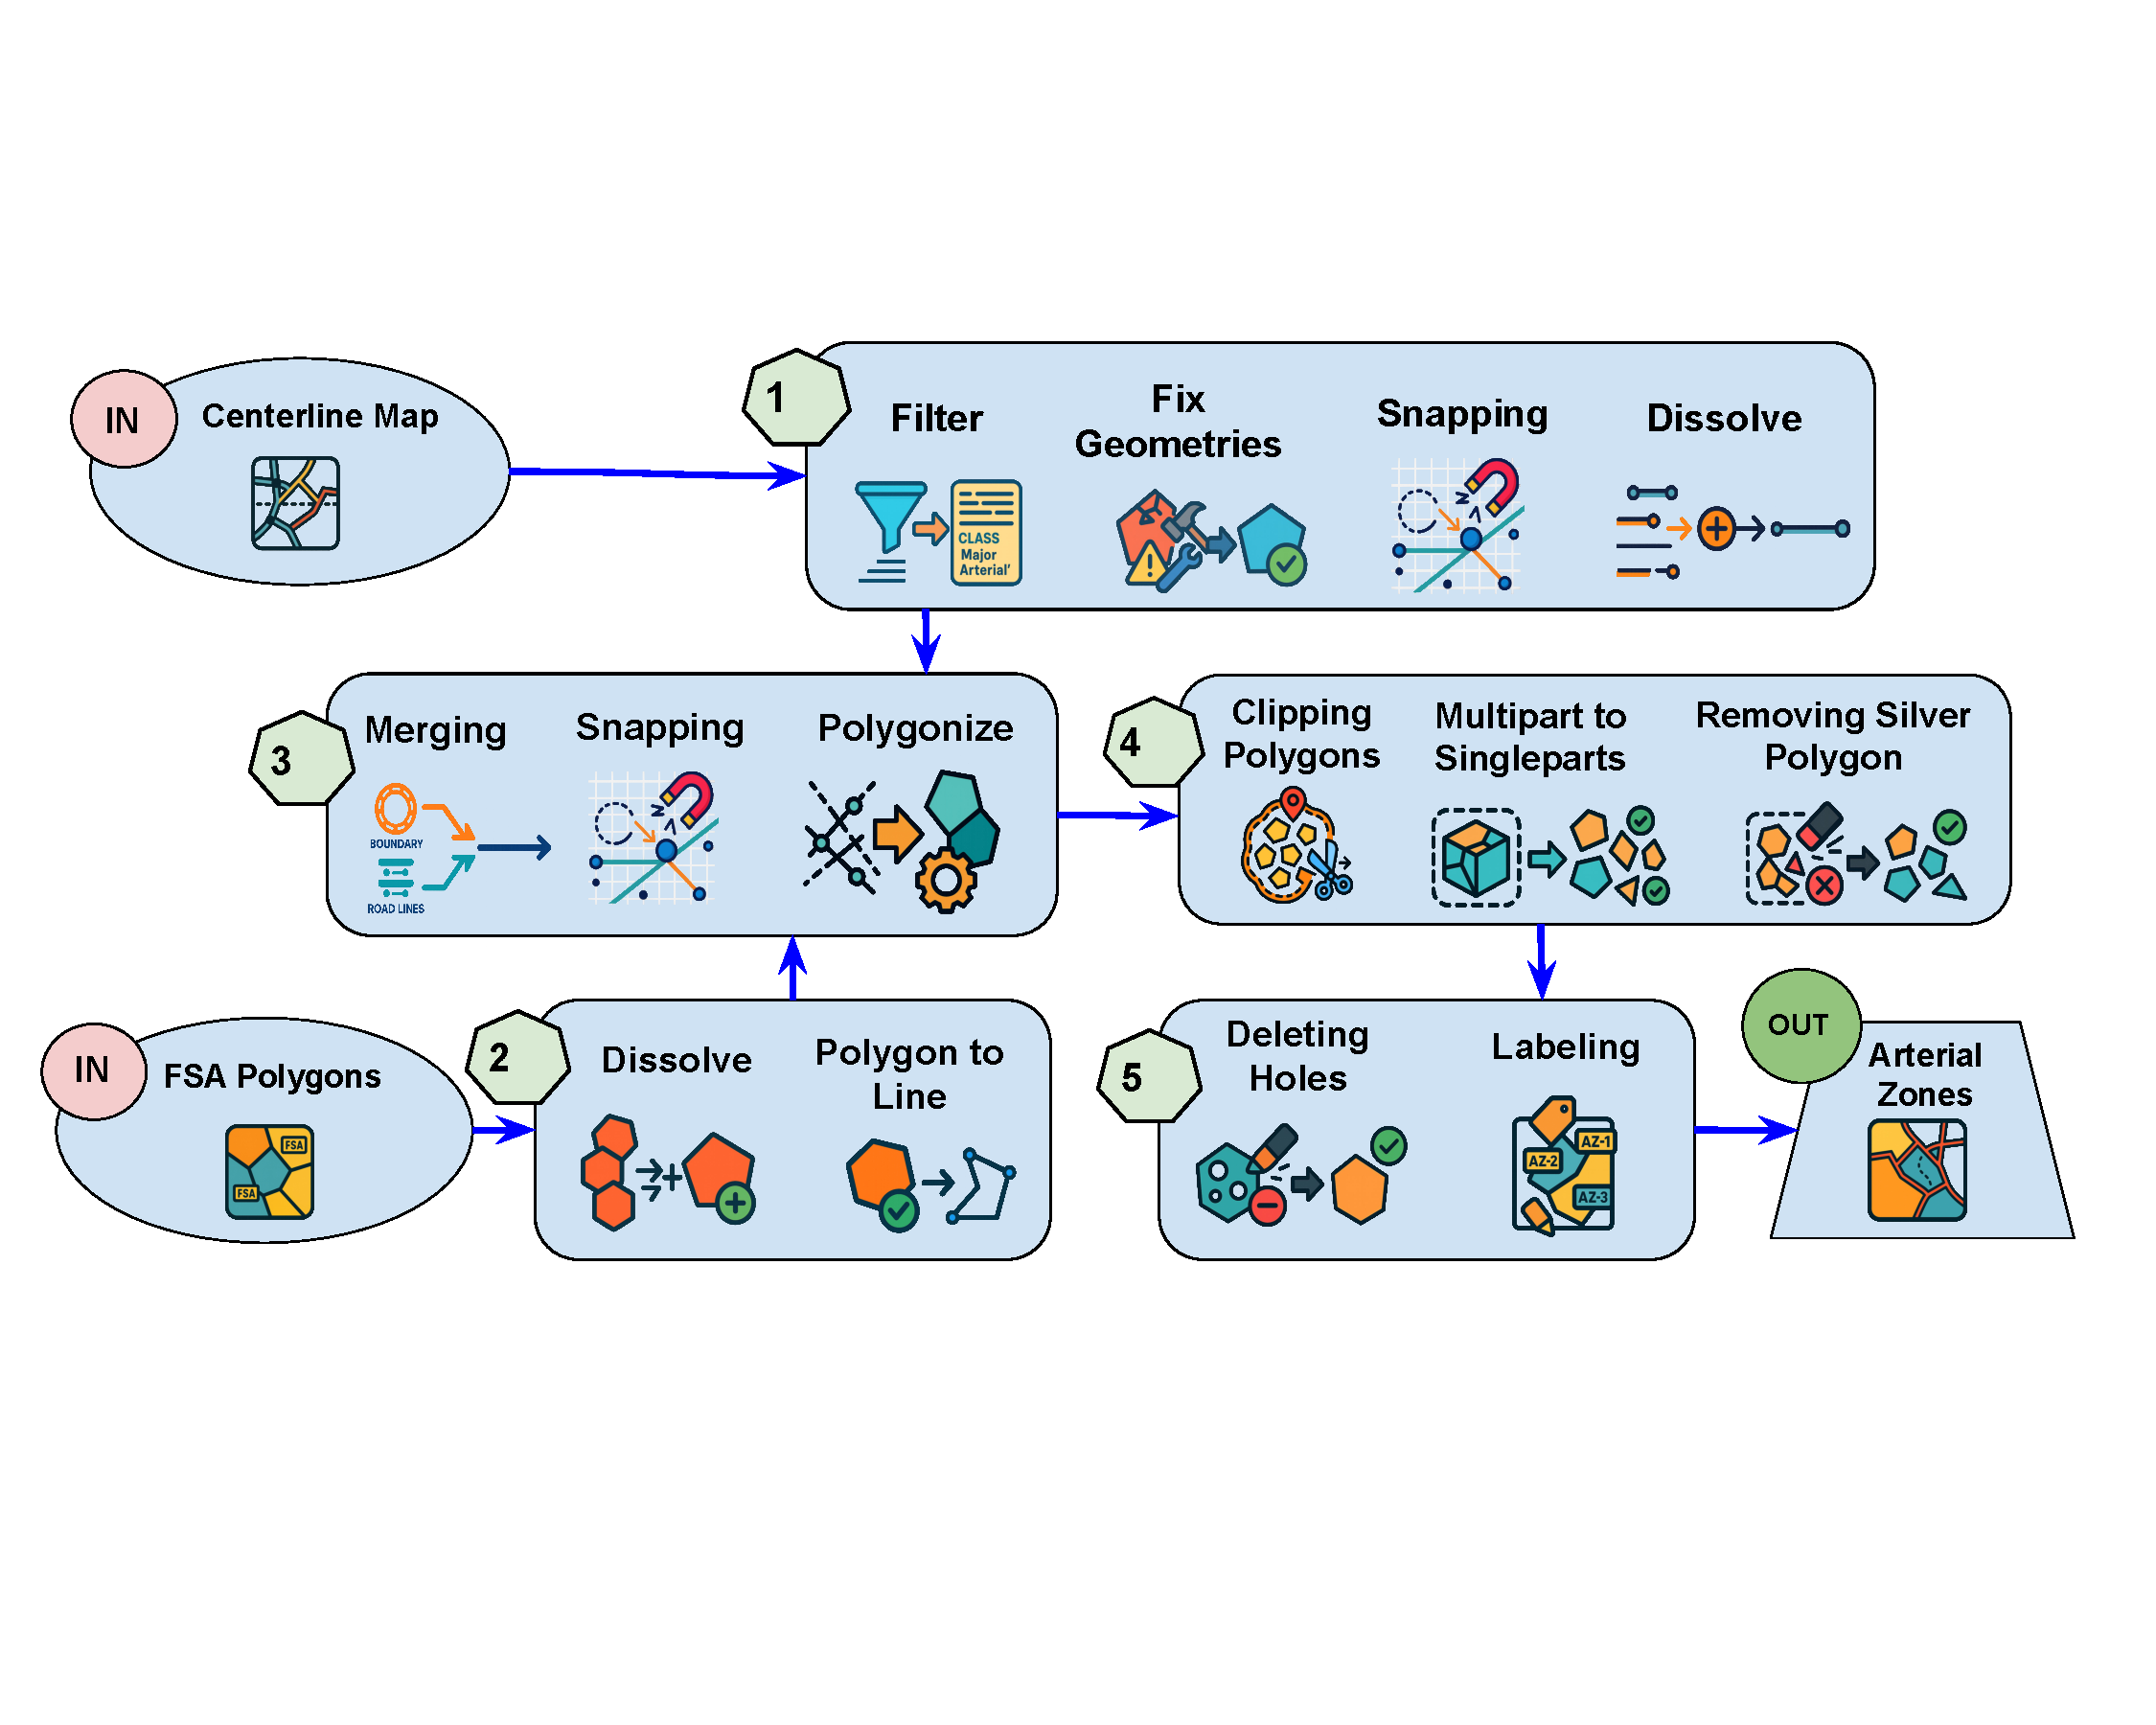
\includegraphics[clip, trim=0.5cm 9.25cm 0.5cm 5.5cm, width=0.9\textwidth]{images/arterial_zoning.pdf}
\caption{Workflow of the arterial zoning algorithm. Road centrelines and \gls{fsa} polygons are processed to produce a set of finalized arterial zones, \gls{ZAr}.}
\label{fig:arterial_zoning_pipeline}
\end{figure}


% \begin{enumerate}
%   \item \textbf{Filter the centreline to major arterials.}
%     \begin{itemize}
%       \item \emph{Layer} $\rightarrow$ \emph{Filter} (or Field Calculator / Select by Expression) with your schema, e.g.:
%       \[
%         \texttt{"CLASS" IN ('Major Arterial','Minor Arterial')}
%       \]
%       (Use your exact field names; definitions align with Table~\ref{tab:road_classes}.)
%       \item \emph{Vector} $\rightarrow$ \emph{Geometry} $\rightarrow$ \textbf{Fix geometries}.
%       \item \emph{Vector} $\rightarrow$ \emph{Geometry} $\rightarrow$ \textbf{Snap geometries} (tolerance \(\sim\) 0.5–1.0~m; to itself) to close micro-gaps that block polygonization.
%       \item \emph{Vector} $\rightarrow$ \emph{Geoprocessing} $\rightarrow$ \textbf{Dissolve} (no dissolve field) to produce a single multiline arterial network (optional but helps polygonization).
%     \end{itemize}

%   \item \textbf{Build the urban boundary from FSAs.}
%     \begin{itemize}
%       \item \emph{Vector} $\rightarrow$ \emph{Geoprocessing} $\rightarrow$ \textbf{Dissolve} on FSA polygons (no field) to create a single \emph{urban boundary} polygon.
%       \item \emph{Vector} $\rightarrow$ \emph{Geometry} $\rightarrow$ \textbf{Polygon to lines} to convert the urban boundary to a line layer (\(\partial\Omega\)).
%     \end{itemize}

%   \item \textbf{Create a planar subdivision bounded by arterials and the urban limit.}
%     \begin{itemize}
%       \item Merge the \emph{arterial lines} with the \emph{boundary lines}:
%         \emph{Processing Toolbox} $\rightarrow$ \textbf{Merge Vector Layers} (or \textbf{Append}).
%       \item Snap again (\emph{Snap geometries}) using the merged layer as both source and target (same 0.5–1.0~m tolerance).
%       \item \emph{Vector} $\rightarrow$ \emph{Geometry} $\rightarrow$ \textbf{Polygonize}. 
%       \item Result: raw faces of the arrangement \( \mathcal{A} = E_{\text{arterial}} \cup \partial\Omega \).
%     \end{itemize}

%   \item \textbf{Clip and clean the faces.}
%     \begin{itemize}
%       \item \emph{Vector} $\rightarrow$ \emph{Geoprocessing} $\rightarrow$ \textbf{Clip} (input: polygonized faces; overlay: urban boundary polygon).
%       \item \emph{Vector} $\rightarrow$ \emph{Geometry} $\rightarrow$ \textbf{Multipart to singleparts}.
%       \item Remove slivers: \emph{Select by Expression} 
%       \[
%         \texttt{\$area < 10\,000} 
%       \]
%       (e.g., $<1$\,ha) $\rightarrow$ delete, or use \textbf{Eliminate sliver polygons} (if available).
%       \item \emph{Vector} $\rightarrow$ \emph{Geometry} $\rightarrow$ \textbf{Delete holes} (threshold e.g., $< 2\,000$\,m\(^2\)) to clean micro-voids.
%     \end{itemize}

%   \item \textbf{Label and finalize arterial zones.}
%     \begin{itemize}
%       \item Add fields via Field Calculator: 
%         \texttt{ZONE\_ID} (e.g., \texttt{'AZ\_' || to\_string(@row\_number)}), 
%         \texttt{AREA\_M2 = \$area}, 
%         \texttt{PERIM\_M = \$perimeter}.
%       \item (Optional) Keep only polygons whose boundaries are mostly arterial: compute the fraction of each face’s perimeter coincident with arterial lines (Overlay \(\rightarrow\) \textbf{Line dissolve} on arterials, then \textbf{Line\_intersections}/\textbf{Line\_locate\_along\_geometry}); filter if needed.
%       \item Export the result as \texttt{arterial\_zones.gpkg} (or shapefile).
%     \end{itemize}
% \end{enumerate}

% \paragraph{Parameter notes (practical and strict).}
% \begin{itemize}
%   \item \textbf{Snapping tolerance:} 0.5–1.0 m typically prevents micro-gaps that break polygonization without over-merging nearby vertices.
%   \item \textbf{Sliver threshold:} Set by map scale and use case. For city-scale zones, $10\,000$–$20\,000$ m\(^2\) is a sensible starting point; tune based on QA.
%   \item \textbf{Topology QA:} If polygonize fails or yields holes, revisit \textbf{Fix geometries} and \textbf{Snap geometries}; inspect dangling ends and overlaps.
% \end{itemize}

\subsection{From \gls{fsa}-level \gls{bev} counts to arterial zones' \gls{bev} densities}\label{sec:Ev_density_for AZ}
Data on vehicle ownership for \gls{bev}s are only available at the \gls{fsa} level, which is the primary record of registered vehicles. Ideally, if ownership data were available at multiple administrative levels, the most detailed unit would be preferred, as higher-resolution data allows for a more accurate representation of spatial variations in \gls{bev} ownership. This improves the allocation of resources to arterial zones and aligns better with major mobility patterns.
The \gls{fsa} polygons are used as the base administrative units. However, \glspl{fsa} do not correspond with mobility corridors and thus do not accurately reflect \gls{bev} activity along major arterial roads. Each \gls{fsa} is intersected with the defined arterial zones, allowing the proportional redistribution of \gls{bev} counts from \gls{fsa} zones to mobility-based arterial zones. This process ensures that \gls{bev} activity is accurately represented within the arterial zones, which serve as the fundamental spatial framework for planning \gls{fc} infrastructure.
The set of intersection regions, denoted by \gls{Zcap}, is defined as
\begin{align}
  \mathcal{Z}^{\cap} 
  \;=\; \bigl\{\, Z^{\cap}_{i,j} \;=\; Z^{\mathrm{FSA}}_i \cap Z^{\mathrm{Ar}}_j \;:\; (i,j)\in\mathcal{K} \,\bigr\}
  \;\subset\; \mathcal{P}(\mathbb{R}^2).
  \label{eq:intersections set}
\end{align}
The index set of valid intersections, \gls{K}, is given by
\begin{align}
  \mathcal{K} \;=\; 
  \bigl\{\, (i,j) \in \mathcal{I}\times\mathcal{J} \;:\;
  \mathrm{Area}\bigl(Z^{\mathrm{FSA}}_i \cap Z^{\mathrm{Ar}}_j\bigr) > 0 \,\bigr\}.
\end{align}
Each \gls{Zcapij} corresponds to a non-empty intersection polygon between the $i$-th \gls{fsa} and the $j$-th arterial zone, that is, all regions where $Z^{\mathrm{FSA}}_i \cap Z^{\mathrm{Ar}}_j$ has positive area.

Let \gls{Area} denote the area functional, which assigns a nonnegative area value to any planar region.
For each \gls{fsa} zone and arterial zone, the corresponding areas are expressed as 

\begin{align}
  A^{\mathrm{FSA}}_i &= \mathrm{Area}\!\left(Z^{\mathrm{FSA}}_i\right), \qquad i \in \mathcal{I}, \label{eq:fsa areas} \\
  A^{\mathrm{Ar}}_j  &= \mathrm{Area}\!\left(Z^{\mathrm{Ar}}_j\right), \qquad j \in \mathcal{J}, \label{eq:artertal_zones_area} \\
  A^{\cap}_{i,j}     &= \mathrm{Area}\!\left(Z^{\mathrm{FSA}}_i \cap Z^{\mathrm{Ar}}_j\right), 
  \qquad (i,j) \in \mathcal{K}, \label{eq:intersections area}
\end{align}
where \gls{Acap} denotes the area of each intersection region between them.
The corresponding set of intersection areas, denoted by \gls{Acapset}, is defined as 
\begin{align}
  \mathcal{A}^{\cap}
  \;=\; \bigl\{\, A^{\cap}_{i,j} 
  :\; (i,j)\in\mathcal{K} \,\bigr\}
  \;\subset\; \mathbb{R}_{\ge 0}.
\end{align}
% Each FSA polygon is then intersected with the arterial regions obtained in the previous step. 
% This ensures that EV counts are spatially redistributed according to the overlap between FSAs and arterial regions. 
% Based on these intersections, the share of EVs belonging to each FSA is allocated to the intersected regions by weighting the EV count of the FSA according to the relative area, i.e.,
The \gls{fsa}-level \gls{bev} counts are redistributed to the intersection regions~\eqref{eq:intersections set} in proportion to their relative areas, as specified by~\eqref{eq:fsa areas} and~\eqref{eq:intersections area}, with the allocation given in~\eqref{eq:EV_allocation_intersection}:
\begin{align}  \label{eq:EV_allocation_intersection}
    \mathrm{EVC}_{i \cap j} \;=\;
    \frac{A^{\cap}_{i,j}}{A^{\mathrm{FSA}}_i} \,\times\, EVC_i,
    \qquad (i,j) \in \mathcal{K},
\end{align}
Here, \gls{EVCcap} denotes the portion of the \gls{bev} count from \gls{fsa}~$i$ that is allocated to the intersection region \gls{Zcapij}.
The set of \gls{bev} counts allocated to intersection regions, denoted by \gls{EVCcapset}, is defined as
\begin{equation} 
\label{eq:ev_counts_for_intersection}
  \mathcal{E}^{\cap}
  \;=\; \bigl\{\, \mathrm{EVC}_{i \cap j} 
  : (i,j)\in\mathcal{K} \,\bigr\}
  \;\subset\; \mathbb{R}_{\ge 0},
\end{equation}
% where each element $\mathrm{EVC}_{i \cap j}$ is given by~\eqref{eq:EV_allocation_intersection} and represents 
% the share of \gls{bev}s from FSA~$i$ assigned to the intersection region $Z^{\cap}_{i,j}$.
The aggregate \gls{bev} count for each arterial region, denoted by \gls{EVCAr}, is obtained by summing the allocated intersection shares over all \glspl{fsa} that intersect the $j$-th arterial zone (\gls{ZArj}), defined as
\begin{equation}
  \label{eq:EV_aggregate_arterial}
  \mathrm{EVC}^{\mathrm{Ar}}_{j}
  \;=\;
  \sum_{i:\,(i,j)\in\mathcal{K}} \mathrm{EVC}_{i \cap j},
  \qquad j \in \mathcal{J}.
\end{equation}
Aggregation of the arterial-level \gls{bev} counts yields the set \gls{EVCArset}, defined as
\begin{equation}
  \mathcal{E}^{\mathrm{Ar}}
  \;=\;
  \bigl\{\, \mathrm{EVC}^{\mathrm{Ar}}_{j} : j \in \mathcal{J} \,\bigr\}
  \;\subset\; \mathbb{R}_{\ge 0}.
\end{equation}
To standardize across zones of varying size, the \gls{bev} density for each arterial zone, denoted by \gls{rhoAr}, is defined as
\begin{align}
  \label{eq:EV_density_arterial}
  \rho^{\mathrm{Ar}}_{j}
  \;=\;
  \frac{\mathrm{EVC}^{\mathrm{Ar}}_{j}}{A^{\mathrm{Ar}}_{j}},
  \qquad j \in \mathcal{J}, \; A^{\mathrm{Ar}}_{j}>0.
\end{align}
For comparability across regions, the \gls{bev} densities are rescaled to the unit interval through min–max normalization. The normalized density for each arterial region, denoted by \gls{rhoArHat}, is defined as
\begin{align}
  \label{eq:EV_density_norm}
  \widehat{\rho}^{\mathrm{Ar}}_{j}
   \;=\;
   \frac{\rho^{\mathrm{Ar}}_{j} - \min_{k \in \mathcal{J}} \rho^{\mathrm{Ar}}_{k}}
        {\max_{k \in \mathcal{J}} \rho^{\mathrm{Ar}}_{k} - \min_{k \in \mathcal{J}} \rho^{\mathrm{Ar}}_{k}},
   \qquad j \in \mathcal{J},
\end{align}
which ensures $\widehat{\rho}^{\mathrm{Ar}}_{j} \in [0,1]$ for all $j$. The set of normalized \gls{bev} densities for all arterial zones, denoted by \gls{rhoArNormSet}, is defined as
\begin{align}
  \label{eq:EV_density_norm_set}
  \widehat{\mathcal{R}}^{\mathrm{Ar}}
   \;=\;
   \bigl\{\, 
      \widehat{\rho}^{\mathrm{Ar}}_{j} 
      : j \in \mathcal{J} 
   \,\bigr\}.
\end{align}
\subsection{Graph construction and hop distance}
\label{subsec:hop_distance}
To represent spatial connectivity among arterial zones, an undirected planar adjacency graph \gls{GraphG} is constructed.
Each arterial zone \gls{ZArj} corresponds to a vertex \gls{VertexVj}, whose position is defined by the geometric centroid functional \gls{Centroid}.
The graph is defined as
\begin{align}
G=(V,E,W),\qquad 
V=\{\,v_j : j\in\mathcal{J}\,\},\;\; v_j \leftrightarrow \mathrm{Centroid}(Z^{\mathrm{Ar}}_j),\label{eq:urban_graph}
\end{align}
where \gls{VertexSet} denotes the set of vertices, \gls{EdgeSet} represents the set of undirected edges, and \gls{WeightMatrix} contains the edge weights.
Two arterial zones are considered adjacent if they share a boundary of positive length.
Let \gls{Boundary} denote the boundary operator and \gls{Length} the boundary-length functional, both computed under the working projection defined in \ref{def:projection}.
The binary adjacency matrix \gls{AdjacencyMatrix} represents the topological connectivity between arterial zones.
Each element \gls{AdjacencyAjk} indicates whether two zones share a common boundary of positive length, defined as

\begin{align}
\label{eq:adjacency_unweighted_fixed}
A_{jk}
=\begin{cases}
1, & \mathrm{Length}\!\bigl(\partial Z^{\mathrm{Ar}}_j \cap \partial Z^{\mathrm{Ar}}_k\bigr) > 0,\ j\neq k,\\[0.25em]
0, & \text{otherwise},
\end{cases}
\qquad j,k \in \mathcal{J},\quad A_{jj}=0.
\end{align}
The weighted adjacency matrix \gls{WeightMatrix} encodes the geometric strength of connections between arterial zones.
Each element \gls{WeightedElement} represents the length of the shared boundary between the two arterial zones \gls{ZArj} and $Z^{\mathrm{Ar}}_k$, defined as
\begin{align}
\label{eq:adjacency_weight_fixed}
w_{jk}
=\mathrm{Length}\!\bigl(\partial Z^{\mathrm{Ar}}_j \cap \partial Z^{\mathrm{Ar}}_k\bigr),
\qquad j,k \in \mathcal{J},\quad w_{jk}=w_{kj}\ge 0,\quad w_{jj}=0.
\end{align}

The hop distance \gls{HopDistance} measures the topological separation between two arterial zones in the unweighted adjacency graph.
It is defined as the number of edges in the shortest path between vertices \gls{VertexVj} and $v_k$ in the graph \gls{GraphG} is defined as
\begin{align}
\label{eq:hop_distance}
d_G(j,k)
=\min_{\pi:j\rightsquigarrow k}\; |\pi|,
\end{align}
where \gls{PathPi} denotes a path connecting \gls{VertexVj} and $v_k$ in $G$, and $|\pi|$ is the number of edges in that path. 
If no connecting path exists, $d_G(j,k)=\infty$. 
The one-hop neighbor set \gls{NeighborSet} and its $h$-hop generalization \gls{NeighborSetH} are defined as
\begin{align}
\label{eq:direct_neibours}
N(j)        &= \{\, k\in\mathcal{J} : A_{jk}=1 \,\}, \\
\label{eq:hop_rings}
N^{(h)}(j)  &= \{\, k\in\mathcal{J} : d_G(j,k)=h \,\}, \quad h=0,1,2,\dots
\end{align}
% and the closed $n$-hop ball used in smoothing, as defined in~\eqref{eq:EV_density_nhop_ball}, is

% \begin{equation}
% \label{eq:hop_ball}
% B^{(n)}(j)=\{\, k\in\mathcal{J} : d_G(j,k)\le n \,\}.
% \end{equation}

% \paragraph{Practical notes.}
% (i) Use an equal-area or metrically appropriate projection so that $\mathrm{Length}(\cdot)$ reflects true shared-boundary distances. 
% (ii) Hop distance is combinatorial and ignores $w_{jk}$ by design (weights can be incorporated later via ring weights or stochastic averaging). 
% (iii) Smoothing and aggregation are applied within the connected component containing $j$; if $d_G(j,k)=\infty$, then $k\notin B^{(n)}(j)$ for any finite $n$.


\subsection{Weighted $n$-hop smoothing}
\label{subsec:nhop_smoothing}
% Spatial smoothing replaces each arterial-zone EV density with a local average over its neighbors on the adjacency graph, reflecting spillovers and reducing small-area noise. Concretely, starting from the unsmoothed densities $\rho^{\mathrm{Ar}}_{j}$ in~\eqref{eq:EV_density_arterial}, we compute a smoothed value by averaging over neighboring zones using the weighted $n$-hop ball in~\eqref{eq:EV_density_nhop_weighted}. We smooth for two reasons: (i) EV ownership and charging demand exhibit spatial dependence along corridors and across adjacent neighborhoods, which a local average captures; and (ii) raw densities can be unstable in small or sparsely connected zones, so smoothing borrows strength from neighbors. The hyperparameter $n$ and ring weights control the spatial scale of influence, trading variance reduction against potential over-smoothing.
% Given the arterial zones' EV densities $\rho^{\mathrm{Ar}}_{k}$ from~\eqref{eq:EV_density_arterial}, the $n$-hop distance-sensitive smoothing, uses ring weights over hop shells is \begin{align}
%   \label{eq:EV_density_nhop_weighted}
%   \tilde{\rho}^{\mathrm{Ar}}_{j}(n,\mathbf{w})
%   \;=\;
%   \sum_{h=0}^{n} 
%   w_h \;\frac{1}{\lvert N^{(h)}(j)\rvert}
%   \sum_{k \in N^{(h)}(j)} \rho^{\mathrm{Ar}}_{k},
%   \qquad j \in \mathcal{J},
% \end{align}
%  $N^{(h)}(j)$ is h-hop neibour zones from Equation~\eqref{eq:hop_rings} and choose nonnegative weights 
% $\mathbf{w}=(w_0,\dots,w_n)$ with $\sum_{h=0}^{n} w_h=1$. 

% with the convention that empty rings $N^{(h)}(j)=\varnothing$ are omitted and the remaining
% weights are renormalized.

% \noindent Equation~\eqref{eq:EV_density_nhop_weighted} defines an $n$-hop ring-weighted smoother. 
% For each arterial zone $j$, the set $N^{(h)}(j)=\{\,k\in\mathcal{J}: d_G(j,k)=h\,\}$ collects the zones at $h$ hops from $j$ in the adjacency graph, with $N^{(0)}(j)=\{j\}$. 
% The vector $\mathbf{w}=(w_0,\dots,w_n)$ contains nonnegative ring weights that sum to one, $\sum_{h=0}^{n} w_h=1$, and controls how influence decays with hop distance. 
% Within each ring $N^{(h)}(j)$, the formula first takes the simple average of the unsmoothed densities $\rho^{\mathrm{Ar}}_k$, the inner sum divided by $|N^{(h)}(j)|$, the number of neighborhood zones plus one, and then forms a convex combination of these ring averages across $h=0,\dots,n$ using the weights $w_h$.

% \noindent If $n=0$, then $\tilde{\rho}^{\mathrm{Ar}}_{j}(0,\mathbf{w})=\rho^{\mathrm{Ar}}_{j}$ (no smoothing). If $w_0=\cdots=w_n=\tfrac{1}{n+1}$, uniform ring weights, and every ring is nonempty, the result is the mean of the ring-wise means. If one chooses $w_h \propto |N^{(h)}(j)|$ and renormalizes over $h$ so weights depend on $j$. Empty rings are omitted in practice; when some $N^{(h)}(j)=\varnothing$, the remaining $w_h$ are renormalized to sum to one.
% The operator is a convex average that preserves units (e.g., vehicles/km$^2$) and lies between the minimum and maximum densities observed within the $n$-hop neighborhood. 
% Choosing $\mathbf{w}$ (e.g., geometric decay $w_h \propto \lambda^h$ with $\lambda\in(0,1)$) tunes the spatial scale of influence: larger mass on small $h$ preserves local detail; heavier tails in $h$ emphasize broader corridor- or region-level spillovers.
Spatial smoothing replaces each arterial-zone \gls{bev} density with a locally averaged value over its neighbouring zones in the adjacency graph \gls{GraphG}, thereby capturing spatial spillover effects and reducing small-area variability. 
Starting from the unsmoothed normalized densities \gls{rhoArHat}, the smoothed density for zone $j$, denoted by \gls{rhoArSmooth}, is defined as

\begin{align}
  \label{eq:EV_density_nhop_weighted}
  \tilde{\rho}^{\mathrm{Ar}}_{j}(n,\mathbf{w})
  \;=\;
  \sum_{h=0}^{n} 
  w_h \;\frac{1}{\lvert N^{(h)}(j)\rvert}
  \sum_{k \in N^{(h)}(j)} \widehat{\rho}^{\mathrm{Ar}}_{k},
  \qquad j \in \mathcal{J},
\end{align}
where \gls{NeighborSetH} denotes the $h$-hop neighbour set defined in~\eqref{eq:hop_rings}, $N^{(0)}(j)=\{j\}$, and \gls{WeightVector} is the vector of nonnegative hop weights satisfying $\sum_{h=0}^{n} w_h=1$. 
Neighbour sets with $\lvert N^{(h)}(j)\rvert=0$ are excluded from the computation, and the remaining weights are renormalized accordingly. 
The set of smoothed \gls{bev} densities across all arterial zones, denoted by \gls{rhoArSmoothSet}, is defined as  

\begin{align}
  \label{eq:EV_density_set}
  \widetilde{\mathcal{D}}^{\mathrm{Ar}}(n,\mathbf{w})
   \;=\;
   \bigl\{\, 
      \tilde{\rho}^{\mathrm{Ar}}_{j}(n,\mathbf{w}) 
      : j \in \mathcal{J} 
   \,\bigr\},
\end{align}
which enumerates the smoothed densities \gls{rhoArSmooth}$(n,\mathbf{w})$ 
in~\eqref{eq:EV_density_nhop_weighted} for all arterial zones 
$j \in $ \gls{J}.
Equation~\eqref{eq:EV_density_nhop_weighted} defines an \gls{nHop}-hop weighted smoothing of \gls{bev} densities. The operation proceeds in two steps. First, for each hop distance $h$, the densities of the $h$-hop neighbours of a given zone are averaged uniformly over the corresponding neighbour set. This produces a mean value that reflects the influence of all zones exactly $h$ steps away. Second, these ring-wise averages are combined across hop levels using a convex weight vector \gls{WeightVector}. The result is a weighted mixture of contributions from multiple spatial scales, with $\mathbf{w}$ controlling the relative importance of nearer versus farther neighbours.
 % This construction maintains the original density units (e.g., vehicles/km²). If we set \( n=0 \), we obtain \( \tilde{\rho}^{\mathrm{Ar}}_{j}=\widehat{\rho}^{\mathrm{Ar}}_{j} \), which indicates no smoothing. 
 % Uniform hop weights $w_h=\tfrac{1}{n+1}$, when all neighbour sets are nonempty, produce the mean of the hop-wise means. Choosing $w_h \propto \lvert N^{(h)}(j)\rvert$ and renormalizing over $h$ collapses to the unweighted $n$-hop ball average in~\eqref{eq:EV_density_nhop_ball}. 
The hyperparameters $n$ and $\mathbf{w}$ control the spatial scale of influence, trading variance reduction against potential over-smoothing. A geometric decay scheme, $w_h \propto \lambda^h$ with $\lambda \in (0,1)$, emphasizes local structure while still allowing broader spillover effects.

% The outputs of this stage are visualized through heatmaps of both the raw density $\rho_i$ and the smoothed density $\tilde{\rho}_i$, which reveal spatial variation and hotspots across the arterial zoning system (Figure~\ref{fig:ev_density_heatmap}).

% \begin{figure}[htbp]
% \centering
% \includegraphics[width=0.85\textwidth]{images/EV_density_heatmap.pdf}
% \caption{Heatmap of EV density across arterial regions based on proportional allocation of FSA-level counts.}
% \label{fig:ev_density_heatmap}
% \end{figure}

% \begin{figure}[htbp]
% \centering
% \includegraphics[width=0.75\textwidth]{images/Arteril_EV_Density_heatmap.pdf}
% \caption{Smoothed EV density heatmap using one-hop adjacency diffusion, highlighting density gradients and regional hotspots.}
% \label{fig:smoothed_ev_density_heatmap}
% \end{figure}

\subsection{Ridge paths as \gls{bev} activity backbones}\label{sec:Ridge paths}
Ridge paths are introduced as structural backbones of \gls{bev} activity and charging-demand proxies.
They are extracted from the smoothed \gls{bev} density surface across the city's arterial zones, highlighting the most prominent spines of \gls{bev} movement and concentration.
 Conceptually, they represent concentrated movement patterns and strategic urban corridor zones where charging demand is expected to be greatest. Unlike uniform thresholding methods, ridge paths adapt to the relative peaks in the density field and align with the directional flow of activity. Therefore, they offer a spatially-aware, activity-driven basis for positioning \gls{fc} infrastructure along significant, high-usage urban routes. Ridge paths are defined as sequences of connected areas characterized by a decreasing yet consistently high \gls{bev} density. These paths are formed by tracing downward from local maxima on the density surface, allowing the density to decrease gradually based on a controlled drop ratio. This regulation ensures that small local dips do not prematurely interrupt the paths, thereby maintaining continuity along important high-activity corridor zones. Each resulting ridge path effectively captures a coherent high-flow activity line, acting as a proxy for zones where latent charging corridors exist within the urban.

\subsubsection{Ridge path extraction}
The set of local maxima, denoted by \gls{M}, consists of all arterial zones in \gls{J} whose smoothed densities \gls{rhoAr} are not smaller than those of any neighboring zones \gls{NeighborSet}. Each element of \gls{M} represents an arterial zone that attains a locally dominant demand level within its adjacency neighborhood, thereby serving as a potential origin point for ridge-path extraction in the density field:
\begin{equation}
  \label{eq:local_maxima_set}
  \mathcal{M}
   \;=\;
   \bigl\{\, 
      j \in \mathcal{J} 
      : \tilde{\rho}^{\mathrm{Ar}}_{j}(n,\mathbf{w}) 
        \ge \tilde{\rho}^{\mathrm{Ar}}_{i}(n,\mathbf{w}),\;
        \forall i \in N(j)
   \,\bigr\},
\end{equation}
where \gls{NeighborSet} denotes the set of direct neighbors of arterial zone~$j$ as defined in~\eqref{eq:direct_neibours}.

For each local maximum $v_m \in \mathcal{M} \subseteq V$, where \gls{VertexSet} denotes the the set of nodes in the urban graph, a ridge path, denoted by \gls{rp_m}, is defined as a finite sequence of nodes 
\begin{align}
  \label{eq:ridge_path}
  \mathsf{rp_m} \;=\; (v_m, \dots, v_k, \dots, v_\ell),
\end{align}
such that $v_m \in \mathcal{M}$ is a local maximum from~\eqref{eq:local_maxima_set},
$(v_{k}, v_{k+1}) \in E$ for all $k = m, \dots, \ell$, where \gls{EdgeSet} denotes the the set of edges in the urban graph, and the sequence satisfies the density-drop condition
\begin{align}
   \tilde{\rho}^{\mathrm{Ar}}_{v_{k+1}}(n,\mathbf{w}) 
   \;\ge\; \tilde{\rho}^{\mathrm{Ar}}_{v_{k}}(n,\mathbf{w}) - \Delta,
   \qquad k = m, \dots, \ell,
\end{align}
for a chosen drop tolerance $\Delta > 0$. The parameter \gls{Delta} controls the maximum allowable decline in smoothed \gls{bev} density between consecutive nodes. The set of all ridge paths originating from local maxima constitutes the ridge-path set, denoted by \gls{RP}, and is defined as
\begin{align}
  \label{eq:ridge_path_set}
  \mathcal{RP}
   = \bigl\{\,
      \mathsf{rp_m} = (v_m, \dots, v_\ell)
      \;\big|\;
      v_m \in \mathcal{M},\;
      (v_k, v_{k+1}) \in E
   \,\bigr\}.
\end{align}

A ridge path is constructed by iteratively traversing neighboring zones whose smoothed density remains within a strategy-specific drop tolerance. At iteration $t$ with current node $v_t$, let the feasible neighbor set be defined as
\begin{align}
N_t &= N(v_t)\setminus \{v_m,\dots,v_t\}, 
&
\mathcal{D}_t &= \{\tilde{\rho}^{\mathrm{Ar}}_u : u \in N_t\},
\end{align}
where $N(v_t)$ denotes the adjacency set of $v_t$ in \gls{VertexSet}.
\gls{Nt} collects all unvisited neighbors of the current node $v_t$, 
while \gls{Dt} records the corresponding smoothed density values. 
At each step, the ridge-walking algorithm selects the next node $v_{t+1}$ from 
$N_t$ according to a density-based rule,
\begin{align}
v_{t+1} \;=\; \arg\max_{u \in N_t} \tilde{\rho}^{\mathrm{Ar}}_u
\quad \text{subject to } 
\tilde{\rho}^{\mathrm{Ar}}_u \ge \tilde{\rho}^{\mathrm{Ar}}_{v_t} - \Delta_t,
\end{align}
% where $\Delta_t>0$ is the drop tolerance at step $t$. The statistic $S_t$ and drop allowance \gls{Deltat} depend on the chosen
% strategy $m \in \{\textsc{avg}, \textsc{max}, \textsc{median}, 
% \textsc{std}, \textsc{laplacian}\}$:
The drop allowance \gls{Deltat} is determined according to the selected ridge-walking strategy, denoted by \gls{St}, average, maximum, median, standard deviation, or Laplacian, which defines how local density information is aggregated into an adaptive tolerance threshold  as follows:

\begin{align}
\label{eq:ridge_avg}
\textsc{avg:}       && S_t &= \operatorname{mean}(\mathcal{D}_t),            
& \Delta_t &= \tfrac{\eta}{2}\!\left(\tilde{\rho}^{\mathrm{Ar}}_{v_t}+S_t\right), \\[4pt]
\label{eq:ridge_max}
\textsc{max:}       && S_t &= \max(\mathcal{D}_t),                            
& \Delta_t &= \tfrac{\eta}{2}\!\left(\tilde{\rho}^{\mathrm{Ar}}_{v_t}+S_t\right), \\[4pt]
\label{eq:ridge_median}
\textsc{median:}    && S_t &= \operatorname{median}(\mathcal{D}_t),           
& \Delta_t &= \tfrac{\eta}{2}\!\left(\tilde{\rho}^{\mathrm{Ar}}_{v_t}+S_t\right), \\[4pt]
\label{eq:ridge_std}
\textsc{std:}       && S_t &= \operatorname{std}(\mathcal{D}_t),              
& \Delta_t &= \eta\,S_t, \\[4pt]
\label{eq:ridge_laplacian}
\textsc{laplacian:} && S_t &= \tilde{\rho}^{\mathrm{Ar}}_{v_t}-\operatorname{mean}(\mathcal{D}_t), 
& \Delta_t &= \eta\,S_t.
\end{align}

% $\eta$ is a scaling hyperparameter that calibrates the threshold $\Delta_t$ across different strategies, thereby controlling the ridge-walker's balance between strictness and flexibility.
The scaling hyperparameter \gls{eta} calibrates the threshold \gls{Deltat} across different strategies, thereby controlling the ridge-walker's balance between strictness and flexibility.
The candidate set of admissible neighbors, denoted by \gls{Ct}, is defined as

\begin{equation}
\mathcal{C}_t = 
\{\,u \in N_t : 
   \tilde{\rho}^{\mathrm{Ar}}_{u} \ge \tilde{\rho}^{\mathrm{Ar}}_{v_t} - \Delta_t \,\}.
\end{equation}
If $\mathcal{C}_t = \varnothing$, the walk terminates. Otherwise, we set
\begin{equation}
v_{t+1} \in \arg\max_{u \in \mathcal{C}_t}\tilde{\rho}^{\mathrm{Ar}}_{u},
\end{equation}
append $v_{t+1}$ to the path, and continue until reaching the maximum 
walk length \gls{L} or termination. To limit the extent of such paths, A maximum walk length, denoted as \gls{L}, is established to control the extent to which a ridge path can extend within the graph.
This constraint prevents excessively long ridge paths that could lose clarity and interpretability as concentrated activity corridor zones.
To maintain consistency with the network structure, \gls{L} is bounded above by the diameter of the graph:
\begin{align}
\operatorname{diam}(G) = \max_{u,v \in V} d_G(u,v),
\end{align}
where \gls{dGuv} represents the hop distance, defined as the length of the shortest path between nodes $u$ and $v$ in the graph.
Given that no ridge path can exceed this limit, we require
\begin{align}
    L &\;\leq\; \operatorname{diam}(G).
\end{align}
To localize ridge-path extraction and prevent unrealistically long trajectories, the maximum walk length \gls{L} is defined as a fraction of the graph diameter \gls{diamG}, scaled by the proportionality factor \gls{alpha}:
\begin{align}
    L &= \alpha \cdot \operatorname{diam}(G),
    \qquad \alpha \in (0,1].
\end{align}
Here, \gls{alpha} controls the relative extent of ridge paths with respect to the overall network size.
Beyond the maximum walk length, ridge-path construction is further constrained by a density-based stopping criterion. Specifically, the walk continues until the average smoothed density along the traversed ridge falls below a prescribed threshold \gls{rhoMin}, defined as the 75th percentile of the \gls{bev} density distribution across all arterial zones. A candidate ridge path \gls{rp_m} is retained only if its mean density satisfies
\begin{align}
\frac{1}{\ell+1}\sum_{i=m}^{\ell+m} \tilde{\rho}^{\mathrm{Ar}}_{v_i} 
\;\geq\; \bar{\rho}_{\min}.
\end{align}


% \subsubsection*{Ridge Extraction: Strategy Family and Hyperparameterized Pipeline}

% Let $G=(V,E)$ be the arterial adjacency graph, and let $\rho^{\mathrm{Ar}}_v$ denote the (raw or smoothed) EV density at node $v\in V$. For a starting peak $s\in V$, a \emph{ridge walker} constructs a path 
% \(
% \mathsf{path}=(v_0,v_1,\dots,v_\ell)
% \)
% with $v_0=s$ by iteratively moving to a neighbor that maintains a bounded drop relative to the current node under a strategy-specific tolerance. We use two global hyperparameters: the maximum walk length $L\in\mathbb{N}$ and the drop tolerance parameter $\eta>0$. After path construction, paths are retained only if their average density exceeds a screening threshold $\bar{\rho}_{\min}$.

% \paragraph{Strategy-specific drop rules.}
% At step $t$, with current node $v_t$ and neighbor set $N(v_t)$, let the neighbor densities be 
% \(
% \mathcal{D}_t=\{\rho^{\mathrm{Ar}}_u: u\in N(v_t)\}.
% \)
% Define a strategy statistic $S_t$ on $\mathcal{D}_t$ and a drop allowance $\Delta_t$ as follows:
% \begin{align*}
% \textsc{avg:}       && S_t &= \operatorname{mean}(\mathcal{D}_t),            & \Delta_t &= \tfrac{\eta}{2}\!\left(\rho^{\mathrm{Ar}}_{v_t}+S_t\right),\\
% \textsc{max:}       && S_t &= \max(\mathcal{D}_t),                            & \Delta_t &= \tfrac{\eta}{2}\!\left(\rho^{\mathrm{Ar}}_{v_t}+S_t\right),\\
% \textsc{median:}    && S_t &= \operatorname{median}(\mathcal{D}_t),           & \Delta_t &= \tfrac{\eta}{2}\!\left(\rho^{\mathrm{Ar}}_{v_t}+S_t\right),\\
% \textsc{std:}       && S_t &= \operatorname{std}(\mathcal{D}_t),              & \Delta_t &= \eta\,S_t,\\
% \textsc{laplacian:} && S_t &= \rho^{\mathrm{Ar}}_{v_t}-\operatorname{mean}(\mathcal{D}_t), \quad & \Delta_t &= \eta\,S_t.
% \end{align*}
% The next node is chosen from the candidate set
% \[
% \mathcal{C}_t \;=\; \left\{\, u\in N(v_t)\setminus \{v_0,\dots,v_t\} \;:\; \rho^{\mathrm{Ar}}_{u} \ge \rho^{\mathrm{Ar}}_{v_t}-\Delta_t \,\right\},
% \]
% by taking the highest-density admissible neighbor:
% \(
% v_{t+1} \in \arg\max_{u\in \mathcal{C}_t}\rho^{\mathrm{Ar}}_u.
% \)
% The walk stops if $\mathcal{C}_t=\varnothing$ or when $t=L-1$.

% \begin{algorithm}[H]
% \caption{Hyperparameterized Ridge Extraction with Strategy Set}
% \label{alg:ridge_extraction}
% \DontPrintSemicolon
% \KwIn{Graph $G=(V,E)$ with densities $\rho^{\mathrm{Ar}}_v$; set of local maxima $\mathcal{P}\subseteq V$; strategy set $\mathcal{M}=\{\textsc{avg},\textsc{max},\textsc{median},\textsc{std},\textsc{laplacian}\}$; max steps $L$; drop parameter $\eta>0$ (or per-strategy $\eta_m$); average-density threshold $\bar{\rho}_{\min}$.}
% \KwOut{Dictionary $\mathsf{StrategyRidges}$ mapping $m\in\mathcal{M}$ to retained ridge paths and annotations.}

% $\mathsf{StrategyRidges}\leftarrow \{\}$\;
% \ForEach{$m\in \mathcal{M}$}{
%   $\mathsf{Ridges}\leftarrow [\,]$, \quad $\mathsf{Annot}\leftarrow [\,]$\;
%   \ForEach{$s\in \mathcal{P}$}{
%     $\mathsf{path}\leftarrow [s]$, \; $\mathsf{visited}\leftarrow \{s\}$, \; $v\leftarrow s$\;
%     \For{$t\leftarrow 0$ \KwTo $L-1$}{
%       $\mathcal{N}\leftarrow N(v)\setminus \mathsf{visited}$\;
%       \If{$\mathcal{N}=\varnothing$}{\textbf{break}}
%       Compute $\mathcal{D}=\{\rho^{\mathrm{Ar}}_u: u\in \mathcal{N}\}$\;
%       Compute $S$ and $\Delta$ according to strategy $m$ \tcp*{see rules above}
%       $\mathcal{C}\leftarrow \{u\in \mathcal{N}: \rho^{\mathrm{Ar}}_u \ge \rho^{\mathrm{Ar}}_{v}-\Delta\}$\;
%       \If{$\mathcal{C}=\varnothing$}{\textbf{break}}
%       $v\leftarrow \arg\max_{u\in \mathcal{C}} \rho^{\mathrm{Ar}}_u$\;
%       append $v$ to $\mathsf{path}$; add $v$ to $\mathsf{visited}$\;
%     }
%     \If{$|\mathsf{path}|\ge 2$}{
%       $\bar{\rho}\leftarrow \frac{1}{|\mathsf{path}|}\sum_{u\in \mathsf{path}}\rho^{\mathrm{Ar}}_u$\;
%       \If{$\bar{\rho}\ge \bar{\rho}_{\min}$}{
%         append $(\mathsf{path},\bar{\rho})$ to $\mathsf{Ridges}$\;
%         $u^\star \leftarrow \mathsf{path}[\lfloor |\mathsf{path}|/2\rfloor]$ \tcp*{mid-node for labeling}
%         append $(u^\star,\bar{\rho})$ to $\mathsf{Annot}$\;
%       }
%     }
%   }
%   $\mathsf{StrategyRidges}[m]\leftarrow \{\texttt{ridges}:\mathsf{Ridges},\;\texttt{annot}:\mathsf{Annot}\}$\;
% }
% \Return $\mathsf{StrategyRidges}$\;
% \end{algorithm}
% \noindent\textit{Notes.} (i) $\eta$ acts as a \emph{drop threshold}: larger $\eta$ yields more permissive walks (longer ridges), while smaller $\eta$ enforces stricter descent control. For \textsc{std} and \textsc{laplacian}, $\eta$ functions as a scale multiplier. (ii) The screening threshold $\bar{\rho}_{\min}$ filters out weak or noisy ridges. (iii) The per-strategy $\eta_m$ can be used if different tolerances are desired across $\mathcal{M}$.
% 
% If this condition is violated, the ridge walk terminates. 
This criterion serves as a hyperparameter of the walker algorithm, ensuring that extracted ridge paths remain concentrated within high-activity corridor zones and do not diffuse into sparsely populated regions.
The set of all nodes participating in ridge paths, denoted by \gls{VRP}, is defined as the union of nodes across all ridge paths specified in~\eqref{eq:ridge_path_set}:
\begin{align}
\label{eq:ridge_path_nodes}
\mathcal{V}_{\mathrm{RP}}
\;=\;
\bigcup_{\mathsf{rp_m}\in\mathcal{RP}}
\{\, v_m, \dots, v_\ell \,\}.
\end{align}
Each element of \gls{VRP} represents a centroid of an arterial zone that rests along at least one extracted ridge path, together outlining the spatial footprint of the mobility-based activity structure within the urban graph.

% A ridge-path extraction method is applied to identify EV activity corridors without
% reliance on rasterized demand surfaces. Multi-strategy walkers (average, maximum,
% Laplacian) are employed to trace density ridges from EV ownership distributions. These
% ridge paths are then snapped to the arterial road network, producing demand corridors
% that align both with intensity of EV activity and with underlying mobility structure.

\subsection{Graph-based proximity evaluation}
Corridor zones are represented as nodes positioned along ridge paths, with each node characterized by specific attributes, such as \gls{bev} density acting as a demand proxy and charger density functioning as a supply proxy. Proximity metrics are calculated between ridge-path nodes and charger nodes, using hop-distance measures that are weighted by \gls{bev} density, along with inverse-distance accessibility indices. The effectiveness of this spatial configuration is assessed by comparing it to randomized baseline scenarios, where charger locations are shuffled to create null models for evaluation.

\subsubsection{Charger capacity density as supply proxy}
The supply of charging infrastructure is represented by the aggregate charging capacity assigned to each arterial zone. Let \gls{C} denote the set of charger stations deployed within the study area. Each charger \gls{c} $ \in $ \gls{C} is characterized by a geographic location $\mathrm{loc}(c) \in \mathbb{R}^2$ and a rated capacity $P_c \in \mathbb{R}_{>0}$. Chargers are spatially assigned to arterial zones through the mapping
\begin{align}
  \label{eq:charger_mapping}
  \phi : \mathcal{C} \;\longrightarrow\; \mathcal{J}, 
  \qquad \phi(c) = j \;\;\text{if}\;\; \mathrm{loc}(c) \in Z^{\mathrm{Ar}}_j,
\end{align}
where \gls{J} denotes the index set of arterial zones and 
$Z^{\mathrm{Ar}}_j \subset \mathbb{R}^2$ represents the polygonal footprint of arterial zone $j$. 
Accordingly, each charger \gls{c} is uniquely mapped to the arterial zone that spatially contains it.
% Each charger $c$ is associated with a rated capacity $P_c$. 
% The total charging capacity for zone $j$ is then defined as
% \begin{align}
% \mathrm{Cap}^{\mathrm{Ar}}_{j} 
%    &= \sum_{\substack{c \in \mathcal{C}\\ c \in Z^{\mathrm{Ar}}_j}} P_c .
% \end{align}
% Each charger $c$ is associated with a rated capacity $P_c \in \mathbb{R}_{>0}$.
The subset of chargers located within arterial zone $j$, denoted by \gls{Cj}, is defined as
\begin{align}
  \label{eq:chargers_in_zone}
  \mathcal{C}_j \;=\; \{\, c \in \mathcal{C} \;:\; \mathrm{loc}(c) \in Z^{\mathrm{Ar}}_j \,\}.
\end{align}
% Each element of \gls{Cj} corresponds to an individual charger \gls{c} whose geographic position lies within the spatial boundary of arterial zone $j$.
The total charging capacity assigned to arterial zone $j$, denoted by \gls{CapArj}, is computed as
\begin{align}
  \label{eq:Cap_zone_by_subset}
  \mathrm{Cap}^{\mathrm{Ar}}_{j}
  \;=\;
  \sum_{c \in \mathcal{C}_j} P_c,
  \qquad j \in \mathcal{J}.
\end{align}
% Here, $\mathrm{Cap}^{\mathrm{Ar}}_{j}$ represents the aggregate rated power of all chargers located within zone $j$, providing a quantitative measure of local charging supply.
To standardize across regions of varying size, the charger capacity density for each arterial zone, denoted by \gls{rhoChj}, is defined as
\begin{align}
  \label{eq:Charger_capacity_density}
  \rho^{\mathrm{Ch}}_{j}
  \;=\;
  \frac{\mathrm{Cap}^{\mathrm{Ar}}_{j}}{A^{\mathrm{Ar}}_{j}},
  \qquad j \in \mathcal{J}, \; A^{\mathrm{Ar}}_{j}>0,
\end{align}
where \gls{CapArj} represents the aggregate rated charging capacity allocated to arterial zone $j$, and \gls{AAr} denotes its corresponding surface area. The set of charger capacity densities across all arterial zones, denoted by \gls{SAr}, is defined as
\begin{equation}
  \label{eq:Charger_capacity_density_set}
  \mathcal{S}^{\mathrm{Ar}}
   \;=\;
   \bigl\{\, 
      \rho^{\mathrm{Ch}}_{j} 
      : j \in \mathcal{J} 
   \,\bigr\}.
\end{equation}
% The set \gls{SAr} represents the spatial distribution of charging supply intensities across all arterial zones within the study area.
% This set provides the supply-side distribution of charging capacity densities across the corridor zones, directly comparable to the demand-side \gls{bev} densities in~\eqref{eq:EV_density_set}.
For comparability across regions, the charger capacity densities are rescaled to the unit interval using min--max normalization. The normalized charger capacity density for each arterial zone, denoted by \gls{rhochhatj}, is computed as
\begin{align}
  \label{eq:Charger_capacity_density_norm}
  \widehat{\rho}^{\mathrm{Ch}}_{j}
   \;=\;
   \frac{\rho^{\mathrm{Ch}}_{j} - \min_{k \in \mathcal{J}} \rho^{\mathrm{Ch}}_{k}}
        {\max_{k \in \mathcal{J}} \rho^{\mathrm{Ch}}_{k} - \min_{k \in \mathcal{J}} \rho^{\mathrm{Ch}}_{k}},
   \qquad j \in \mathcal{J},
\end{align}
which ensures that $\widehat{\rho}^{\mathrm{Ch}}_{j} \in [0,1]$ for all $j$. The collection of these normalized values across all arterial zones constitutes the set \gls{SArhat}, representing the spatially standardized distribution of charger capacity densities.
\begin{equation}
  \label{eq:Charger_capacity_density_norm_set}
  \widehat{\mathcal{S}}^{\mathrm{Ar}}
   \;=\;
   \bigl\{\, 
      \widehat{\rho}^{\mathrm{Ch}}_{j} 
      : j \in \mathcal{J} 
   \,\bigr\}.
\end{equation}


\subsubsection{Weighted proximity distance metric}
\label{subsubsec:wpd_metric}
The effectiveness of charging infrastructure in serving high-activity corridor zones, ridge paths' nodes on the arterial-zone graph \gls{GraphG} is assessed.
The nodes of ridge paths capture localized concentrations of \gls{bev} activity, which serve as indicators of charging demand. Meanwhile, charger nodes represent the available supply and capacity for charging. Proximity between these nodes is assessed based on the hop-based structure of the underlying road network rather than using Euclidean distance. To measure the accessibility between demand and supply nodes, the \gls{wpd} is introduced.


For each node $v_j \in \mathcal{V}_{\mathrm{RP}}$, let \gls{cvstar} denote its nearest charger node in terms of hop distance. The accessibility metric, expressed as the \gls{wpd}, is defined by
\begin{align}
\label{eq:wpd}
\mathrm{WPD} \;=\;
\frac{\sum\limits_{v_j \in \mathcal{V}_{\mathrm{RP}}}
    d(v_j, c^*(v_j)) \,\cdot\, \tilde{\rho}^{\mathrm{Ar}}_j \,\cdot\, \max\!\bigl(\widehat{\rho}^{\mathrm{Ch}}_{c^*}, \varepsilon\bigr)}
     {\sum\limits_{v_j \in \mathcal{V}_{\mathrm{RP}}}
    \tilde{\rho}^{\mathrm{Ar}}_j \,\cdot\, \max\!\bigl(\widehat{\rho}^{\mathrm{Ch}}_{c^*}, \varepsilon\bigr)},
\end{align}
where \gls{dvvstar} denotes the hop-based shortest-path distance between the ridge-path node $v_j$ and its nearest charger node \gls{cvstar}, while \gls{rhoArSmooth} represents the smoothed demand density at $v_j$. The parameter $\varepsilon > 0$ is introduced to prevent zero weighting in regions with sparse charger availability, ensuring numerical stability and maintaining the continuity of accessibility evaluation across the network.
This formulation measures accessibility by weighting proximity based on local \gls{bev} density and charger capacity. This approach effectively captures the spatial reach of charging supply across high-activity corridor zones. A smaller value of \gls{wpd} indicates a stronger alignment between ridge-path nodes and charging infrastructure, meaning that high-demand nodes are closer, in terms of hop distance, to adequately equipped chargers. In contrast, larger values of \gls{wpd} signal reduced accessibility, showing that ridge-path nodes are generally farther away from suitable chargers within the network. The computational procedure is described in Algorithm \ref{alg:wpd}.

\subsubsection{Proximity Evaluation Algorithm}
\label{subsubsec:wpd_algorithm}

\begin{algorithm}[H]
\caption{Computation of \gls{wpd}}
\label{alg:wpd}
\begin{algorithmic}[1]
\REQUIRE Graph $G=(V,E, W)$ in~\eqref{eq:urban_graph}; ridge paths nodes $\mathcal{V}_{\mathrm{RP}}\subseteq V$ in~\eqref{eq:ridge_path_set}; charger nodes $\mathcal{C}\subseteq V$ in~\eqref{eq:charger_mapping};
demand weights $\widetilde{\mathcal{D}}^{\mathrm{Ar}}(n,\mathbf{w})$ in~\eqref{eq:EV_density_set}; supply weights $\widehat{\mathcal{S}}^{\mathrm{Ar}}$ in \eqref{eq:Charger_capacity_density_norm_set}; small constant $\varepsilon>0$.
\FOR{each $v_j \in \mathcal{V}_{\mathrm{RP}}$}
  \STATE Compute hop distances $d(v_j,c)$ to all reachable $c \in \mathcal{C}$.
  \STATE Select $c^*(v_j)$ by minimum hop distance.
  \STATE Record $(d(v_j,c^*(v_j)),\, \widehat{\rho}^{\mathrm{Ar}}_j,\, \widehat{\rho}^{\mathrm{Ch}}_c$.
\ENDFOR
\STATE Compute numerator and denominator of~\eqref{eq:wpd} and return \gls{wpd}.
\end{algorithmic}
\end{algorithm}

\subsection{Evaluating charger–activity spatial alignment}
\label{subsec:null_distribution}
% To evaluate the spatial alignment between real-world fast charger locations and \gls{bev} ridge-path activity, a null distribution was constructed to represent the performance expected under purely random infrastructure placements. This baseline enables statistical testing to determine whether the observed charger-activity alignment arises from intentional spatial design or is a chance occurrence. A statistically significant alignment indicates that ridge-paths' \gls{bev} activity effectively represents the underlying spatial structure of charging demand, validating its use as a behavioral proxy for infrastructure planning.
To assess the degree to which real-world \gls{fc} infrastructure align with \gls{bev} high-activity zones, a null distribution was constructed.
This distribution represents the level of alignment we would expect if charger locations were placed randomly. By establishing this randomized baseline, we can conduct statistical tests to determine whether the observed correspondence between charger locations and \gls{bev} high-activity zones is significantly different from what would occur by chance. If the results are statistically significant, it indicates a meaningful relationship between the locations of the chargers and the activity zones, suggesting a deliberate spatial arrangement rather than mere coincidence. This approach allows for a comprehensive assessment of the demand for, and accessibility to, \gls{fc} infrastructure across the city, treating both the charging network and mobility corridors as interconnected components of the urban system.


\subsubsection{Null distribution construction}
The null model preserves two essential characteristics of the real network: the total number of charging stations and the number of charging ports in each charging station. Under these constraints, charger nodes are randomly distributed across the arterial-zones, ensuring that the underlying network topology and \gls{bev} activity surface remain fixed.
For each randomized configuration, the \gls{wpd} is recalculated to quantify accessibility between ridge-paths' nodes and their nearest charging nodes, weighted by both \gls{bev} activity intensity and charger capacity. Let \gls{VChreal} $\subseteq V$ denote the set of real charger locations, where each charger \gls{creal} is assigned a rated capacity \gls{kcreal} $\in$ \gls{Nplus}. Similarly, let \gls{VChrandom} $\subseteq$ \gls{VertexSet} denote the set of randomized charger locations, where each charger \gls{crandom} is assigned a capacity \gls{kcrandom} $\in $ \gls{Nplus}. These randomized configurations serve as null counterparts to the real-world charger set, preserving the overall number and capacity distribution while randomizing spatial placement across the network.
The null model generates randomized configurations subject to the following constraints:
\begin{align}
|\mathcal{V}^{Ch}_{\mathrm{random,r}}| &= |\mathcal{V}^{Ch}_{\mathrm{real}}|, 
&
\sum_{c_{random} \in \mathcal{V}^{Ch}_{\mathrm{random,r}}} k^c_{random} 
&= 
\sum_{c_{real} \in \mathcal{V}^{Ch}_{\mathrm{real}}} k^c_{real}.
\label{eq:null_constraints}
\end{align}
Each \gls{VChrandom} is sampled uniformly from the admissible subsets of \gls{VertexSet} that satisfy~\eqref{eq:null_constraints}, ensuring that the spatial structure of \gls{GraphG}, and the ridge-paths configuration remains fixed throughout the analysis. For each random configuration \gls{VChrandom}, the \gls{wpd} is recalculated as

\begin{align}
\label{eq:wpd_random}
\mathrm{WPD}(\mathcal{V}^{Ch}_{\mathrm{random,r}}) \;=\;
\frac{\sum\limits_{v_j \in \mathcal{V}_{\mathrm{RP}}}
    d_G(v_j, c_r^*(v_j; \mathcal{V}^{Ch}_{\mathrm{random,r}})) \,\cdot\, \tilde{\rho}^{\mathrm{Ar}}_j \,\cdot\, 
    \max\!\bigl(\widehat{\rho}^{\mathrm{Ch}}_{c_r^*}, \varepsilon\bigr)}
     {\sum\limits_{v_j \in \mathcal{V}_{\mathrm{RP}}}
    \tilde{\rho}^{\mathrm{Ar}}_j \,\cdot\, 
    \max\!\bigl(\widehat{\rho}^{\mathrm{Ch}}_{c_r^*}, \varepsilon\bigr)}.
\end{align}
where \gls{RP} denotes the set of ridge path nodes,  
\gls{dGuv} is the shortest-path hop distance on \gls{GraphG}, \gls{crstar} is the nearest charger to $v_j$ in random chargers placement,  
and \gls{rhoChhatRandom} represents the normalized charger capacity density associated with the nearest randomized charger.
The collection of \gls{wpd}$(\mathcal{V}^{Ch}_{\mathrm{random},r})$ values obtained from \gls{R} independent random realizations forms the null distribution, denoted by \gls{M0}:
\begin{align}
\mathcal{M}_0
   = 
    \{\mathrm{WPD}(\mathcal{V}^{Ch}_{\mathrm{random,1}}),\dots\, \mathrm{WPD}(\mathcal{V}^{Ch}_{\mathrm{random,r}}), \dots\,\mathrm{WPD}(\mathcal{V}^{Ch}_{\mathrm{random,R}})\}
\label{eq:null_distribution_formal}
\end{align}
\subsubsection{Elbow analysis for convergence detection}
The reliability of the null distribution \gls{M0} depends on the number of independent random realizations \gls{R}. Let \gls{muR} and \gls{sigmaR} represent the sample mean and standard deviation of \gls{wpd}$(\mathcal{V}^{Ch}_{\mathrm{random},r})$ values obtained after \gls{R} experiments:

\begin{align}
\mu_R &= 
\frac{1}{R}\sum_{r=1}^{R} 
\mathrm{WPD}(\mathcal{V}^{Ch}_{\mathrm{random},r}),
\label{eq:null_mean} \\[4pt]
\sigma_R^2 &= 
\frac{1}{R-1}\sum_{r=1}^{R} 
\bigl(\mathrm{WPD}(\mathcal{V}^{Ch}_{\mathrm{random},r}) - \mu_R\bigr)^2.
\label{eq:null_variance}
\end{align}
Convergence of the null model is achieved when the variation of \gls{muR} with respect to \gls{R} becomes negligibly small,
\begin{align}
\bigl|\,\mu_{R+\Delta R} - \mu_{R}\,\bigr| < \delta,
\label{eq:convergence_condition}
\end{align}
where \gls{delta} denotes a predefined tolerance threshold, indicating that additional random realizations no longer produce a meaningful change in the estimated baseline performance.
This criterion ensures that the empirical null distribution adequately spans the feasible random space and that its statistical moments are stable. In practice, the convergence threshold is determined through an elbow analysis of \gls{muR} as a function of \gls{R}, with the inflection point indicating the minimum number of simulations required for distributional stability.
% , as illustrated in Fig.~\ref{fig:elbow_plot}.
% \begin{figure}[htbp]
% \centering
% 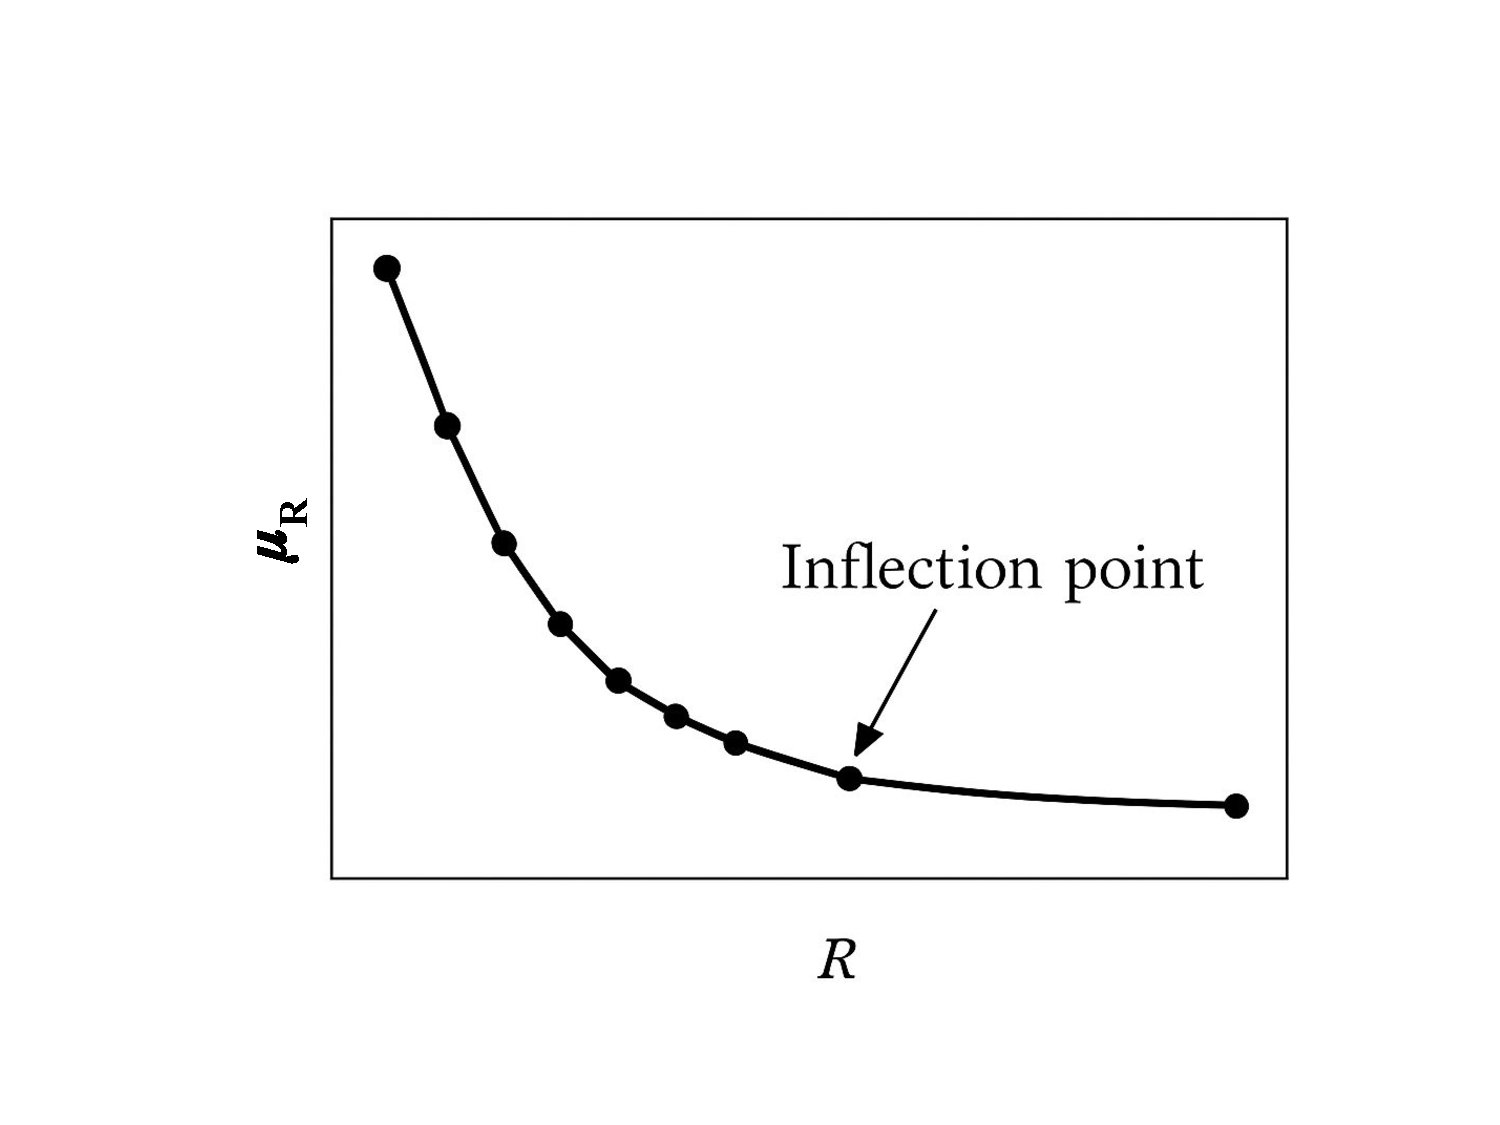
\includegraphics[clip, trim=0.5cm 2.5cm 0.5cm 3.0cm, width=0.9\textwidth]{images/elbow_plot.pdf}
% \caption{
% Elbow analysis of the mean weighted proximity distance $\mu_R$ as a function of the number of random simulations $R$. 
% The inflection point marks the threshold of distributional convergence, beyond which additional simulations yield negligible improvement in baseline stability.
% }
% \label{fig:elbow_plot}
% \end{figure}
The convergence point confirms that the null distribution provides a statistically reliable baseline for assessing charger placement performance relative to random allocation. By comparing the observed proximity metric of the real network to this stabilized null model, statistical significance is evaluated to determine whether the charger network exhibits spatial alignment with \gls{bev} activity corridor zones.
The hypothesis test evaluates whether the real network aligns with ridge-path activity better than random:
\begin{eqnarray}
H_0\!:\! & \mathrm{WPD}_{\mathrm{real}} \sim \mu_R & \quad \text{(no improvement over random)}, \\[4pt]
H_A\!:\! & \mathrm{WPD}_{\mathrm{real}} < \mu_R & \quad \text{(better-than-random alignment)}.
\label{eq:hypothesis_test}
\end{eqnarray}
% Define the empirical $p$-value as
% \begin{align}
% p_{\text{perm}}
% \;=\;
% \frac{1 + \sum_{r=1}^{R} \mathbf{1}\!\left\{\mathrm{WPD}(\mathcal{V}^{Ch}_{\mathrm{random,r}}) \le \mathrm{WPD}_{\mathrm{real}}\right\}}
%      {R + 1},
% \label{eq:p_perm}
% \end{align}
% which is valid without distributional assumptions. Reject $H_0$ at level $\alpha$ if $p_{\text{perm}} \le \alpha$. The parameter $\alpha$ denotes the predefined significance level of the hypothesis test, representing the probability of rejecting the null hypothesis $H_0$ when it is in fact true:
% \begin{align}
% \alpha \;=\; \Pr(\text{reject } H_0 \mid H_0 \text{ is true}).
% \end{align}
% In practical terms, $\alpha$ specifies the maximum tolerated false-positive rate when inferring non-random spatial alignment.  
% A smaller $\alpha$ imposes stricter evidence requirements, reducing the likelihood of false discovery but increasing the risk of overlooking genuine alignment.  
% In this analysis, $\alpha = 0.05$ was adopted to strike a balance between statistical rigor and sensitivity, consistent with conventional standards in spatial and transportation research.
% Let
% \begin{align}
% \mu_R \;=\; \frac{1}{R}\sum_{r=1}^R \mathrm{WPD}(\mathcal{C}_r),
% \qquad
% \sigma_R^2 \;=\; \frac{1}{R-1}\sum_{r=1}^R\bigl(\mathrm{WPD}(\mathcal{C}_r)-\mu_R\bigr)^2.
% \end{align}
% A standardization for interpretability is
% \begin{align}
% z \;=\; \frac{\mathrm{WPD}_{\mathrm{obs}} - \mu_R}{\sigma_R},
% \end{align}
% with (approximate) one-sided $p$-value $p_z = \Phi(z)$ when $\mathcal{N}$ is near-normal.\footnote{Use \eqref{eq:p_perm} for inference; $z$ is for effect interpretation.}
% \paragraph{Effect size (probability of superiority).}
% Let $\mathrm{rank}(\mathrm{WPD}_{\mathrm{obs}})$ be the rank among $\{\mathrm{WPD}_{\mathrm{obs}}, \mathrm{WPD}(\mathcal{C}_1),\dots,\mathrm{WPD}(\mathcal{C}_R)\}$ (1 = best).
% The common-language effect size is
% \begin{align}
% \pi \;=\; \mathbb{P}\!\left(\mathrm{WPD}_{\mathrm{obs}} < \mathrm{WPD}(\mathcal{C}_r)\right)
% \;\approx\;
% \frac{R + 2 - \mathrm{rank}(\mathrm{WPD}_{\mathrm{obs}})}{R+1},
% \end{align}
% interpretable as the fraction of random draws outperformed by the real network.
% \paragraph{Decision rule.}
% Conclude \emph{statistically significant spatial alignment} (non-random placement aligned to ridge-path demand) if $p_{\text{perm}} \le \alpha$ (e.g., $\alpha=0.05$). Report $(p_{\text{perm}}, z, \pi)$ for completeness.
% This evaluation is grounded in the ridge-path \gls{bev} activity representation introduced in Section~\ref{sec:Ridge paths}, which captures \gls{bev} count intensity along arterial corridor zones. 
Integrating mobility-based activity structure with the null distribution framework enables a rigorous statistical test of charger network intentionality, reflecting the extent to which the spatial configuration of chargers exhibits purposeful alignment with \gls{bev} activity corridor zones rather than patterns arising from random placement, forming the empirical foundation for subsequent analyses of efficiency, equity, and spatial optimization.

% Optional linking sentence to next section
% This analysis establishes the statistical foundation for the empirical results presented in Section~\ref{subsec:evaluation_results}.


% The proposed WPD offers practical benefits in a single, interpretable construct: (i) \emph{joint supply--demand weighting}, where distances are modulated by EV demand intensity and charger capacity to highlight consequential gaps; (ii) \emph{network realism}, since hop-based paths respect the arterial topology and avoid misleading Euclidean shortcuts; (iii) a \emph{benchmarkable scalar} that enables direct comparison of deployment scenarios across space and time; and (iv) \emph{diagnostic by-products}, as nearest-charger assignments and path lengths per ridge support spatial audits and equity analyses.

% \subsection{Meso-Level Planning Toolkit}
% The integration of corridor-aligned zoning, ridge-path extraction, and graph-based
% proximity metrics produces a meso-level planning toolkit. This framework bridges
% macro-level adoption forecasting and micro-level site optimization. It enables planners
% to detect misalignments between demand corridors and existing charging networks,
% prioritize corridors for infrastructure rollout, and generate inputs for equity and
% allocation studies at finer scales.


 

% ======================
% Case Study
% ======================
\section{Case study}
\label{sec:case_study}
\subsection{Study area and datasets}
\label{subsec:study_area}
This study focuses on the City of Toronto, Canada, employing arterial corridor zones derived in Section~\ref{sec:derived_AZ}. 
The empirical analysis draws upon three primary datasets: 
(i) The \gls{tcl}, obtained from the City of Toronto Open Data Portal, which provides comprehensive road geometry and functional classifications summarized in Table~\ref{tab:road_classes}; 
(ii) \glspl{fsa}, acquired from Statistics Canada’s Spatial Data Repository, which delineate the urban study boundary and represent the most disaggregated spatial level at which \gls{bev} registration data are available; and 
(iii) FLO \gls{dcfc} stations, sourced from \gls{afdc} database. 
Because the \gls{afdc} dataset does not specify per-port power ratings, a uniform nominal charging power of $100\,\mathrm{kW}$ per port was assumed across all installations. 
% The spatial distribution of these stations was subsequently mapped in accordance with Equation~\ref{eq:charger_mapping}. 

All spatial analyses were conducted using \texttt{QGIS v3.34} and Python \texttt{v3.11}, employing the \texttt{geopandas} and \texttt{networkx} libraries. 
Computations were performed on a 64-bit Windows~10 workstation equipped with an Intel\textsuperscript{\textregistered} Core\textsuperscript{TM} i7-8700T CPU @ 2.40\,GHz, 16\,GB RAM, and integrated Intel UHD Graphics~630. 
Data were stored on a 512\,GB NVMe SSD. 
Typical preprocessing and spatial intersection operations over 234 arterial regions completed within several minutes.
\subsection{Arterial zone extraction}\label{subsec:az_extraction}
The proposed arterial zoning algorithm successfully transformed the \gls{tcl} and \gls{fsa} boundaries, as illustrated in Figure \ref{fig:TCN_FSA}, into a topologically coherent and spatially continuous set of arterial zones shown in Figure \ref{fig:arterial_zones}, suitable for meso-scale spatial analysis. All layers are projected to UTM 17N (EPSG:32617) per Definition~\ref{def:projection}.  Starting from over 40{,}000 individual road segments in the \gls{tcl} dataset, the filtering and connectivity refinement stages reduced the network to approximately 1{,}200 major arterial links. This selective extraction preserved the primary mobility corridors that shape \gls{bev} travel demand while excluding expressway, local and collector roads that fragment the network topology. 
\begin{figure}[htbp]
  \centering
  \captionsetup{justification=centering}
  % (a)
  \begin{subfigure}[t]{0.49\textwidth}
    \centering
    \includegraphics[width=\linewidth,
                     height=0.6\textheight,
                     keepaspectratio,
                     pagebox=cropbox]{images/Toronto_Centreline_JournalMap.pdf}
    \caption{\gls{tcl} dataset, representing the primary road infrastructure used for arterial zones delineation.}
    \label{fig:TCN}
  \end{subfigure}\hfill
  % (b)
  \begin{subfigure}[t]{0.49\textwidth}
    \centering
    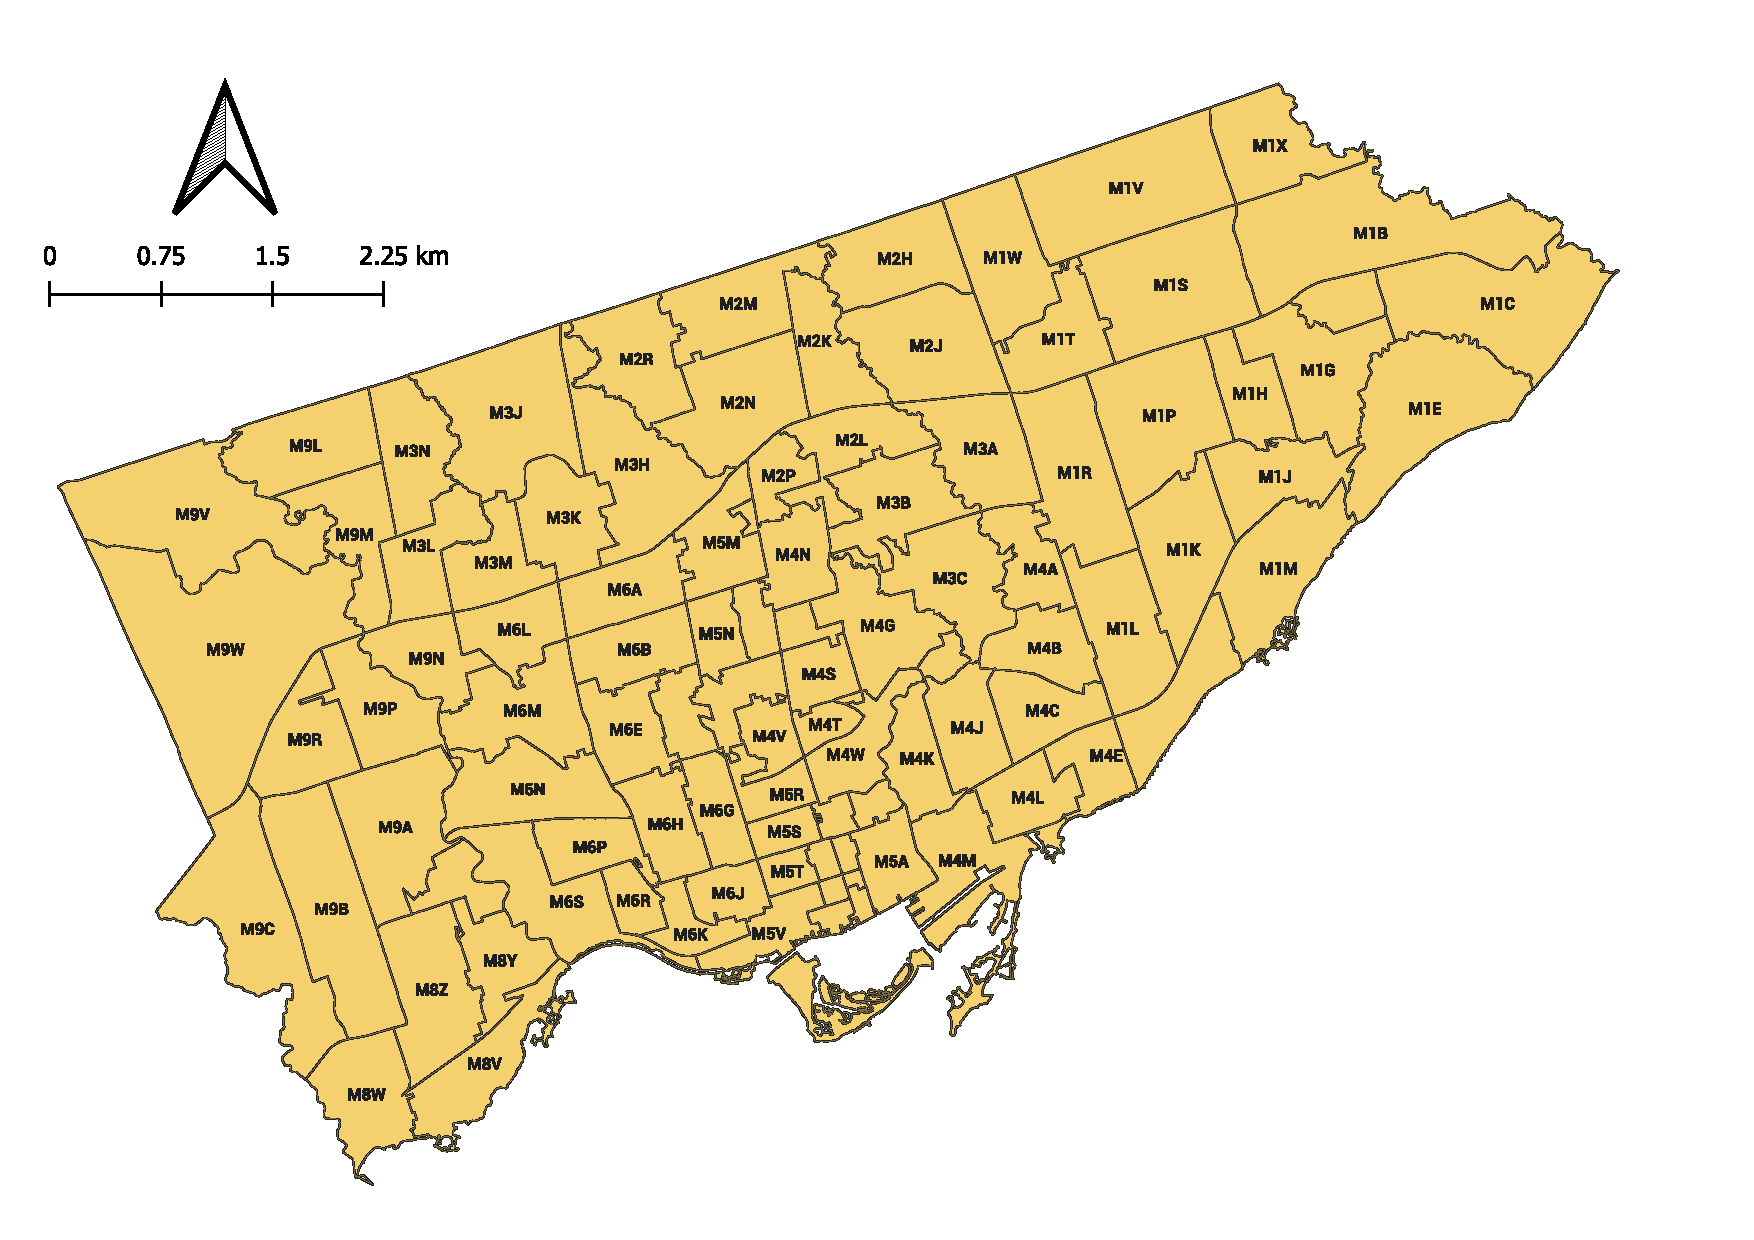
\includegraphics[width=\linewidth,
                     height=0.44\textheight,
                     keepaspectratio,
                     pagebox=cropbox]{images/Toronto_FSA_JournalMap.pdf}
    \caption{\gls{fsa} boundaries, representing the finest spatial level at which \gls{bev} registration data are available in the study area.}
    \label{fig:FSA}
  \end{subfigure}

  \caption{Input geospatial datasets for the arterial zoning algorithm: (a) \gls{tcl} dataset; (b) \gls{fsa} boundaries.}
  \label{fig:TCN_FSA}
\end{figure}

The polygonization process, limited by the dissolved \glspl{fsa} boundaries, produced 234 contiguous arterial zones throughout the urban region, as illustrated in Figure \ref{fig:arterial_zones}.
% Each zone is topologically closed, free of overlaps or sliver geometries, and uniquely labeled according to Equation~\eqref{eq:AZ_final}. 
The resulting zones exhibit a strong spatial alignment with the major arterial roads structure of Toronto, capturing the city’s major east-west and north-south travel corridors such as Bloor, Danforth, Eglinton, Finch, and Lawrence avenues.
% The geometric refinement step removed 17 micro-polygons below the area threshold (0.02~km$^2$), ensuring that all final zones represent meaningful planning units. The average arterial zone area is 2.8~km$^2$, with a standard deviation of 1.6~km$^2$. Larger zones are concentrated in the suburban periphery where arterial spacing increases, while smaller, denser zones emerge in the downtown core where road intersections are frequent and block sizes are smaller.
The final arterial zoning layer  provides a robust spatial framework for subsequent \gls{bev} charging activity modeling and accessibility analysis. Each zone is readily intersectable with demographic, traffic, or infrastructure datasets, enabling consistent aggregation and disaggregation across urban subsystems. Compared to \gls{fsa} or census-based partitions, the arterial zones offer improved geometric regularity and direct correspondence to transportation corridors, which are essential for modeling vehicle-based mobility and charger utilization.
\begin{figure}[htbp]
  \centering
  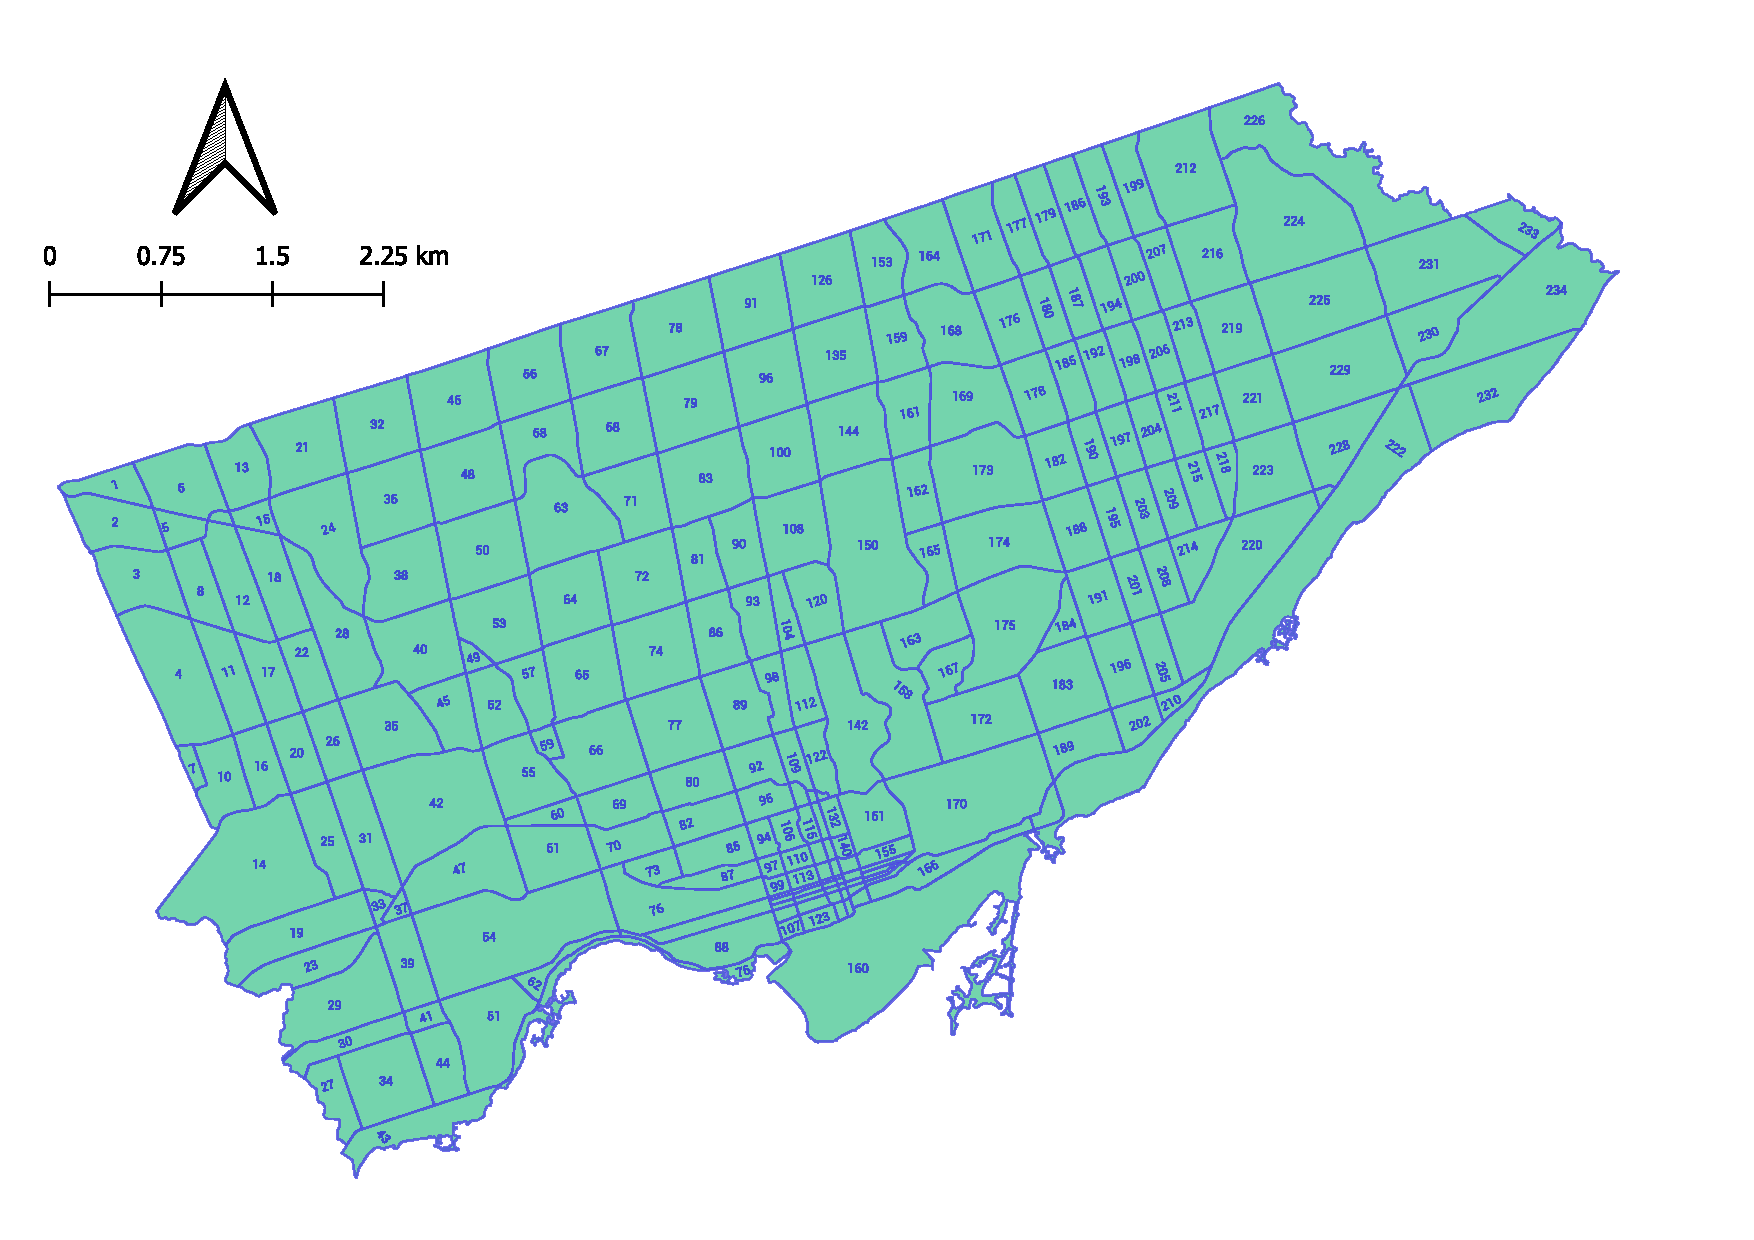
\includegraphics[width=0.75\linewidth]{images/Toronto_arterial_zones_JournalMap.pdf}
  \caption{Derived arterial zones for the City of Toronto.}
  \label{fig:arterial_zones}
\end{figure}
\subsection{Arterial zones' \gls{bev} densities}
\label{subsec:EV_density_results}
The redistribution procedure described in Section~\ref{sec:Ev_density_for AZ} produces spatial field of  \gls{bev} densities aligned with the arterial corridor zones. 
% Figure~\ref{fig:arterial_ev_density} illustrates the resulting distribution of smoothed BEV densities $\tilde{\rho}^{\mathrm{Ar}}_{j}$ across the arterial zones of Toronto, as computed from~\eqref{eq:EV_density_nhop_weighted}. 
By intersecting the \gls{fsa} polygons with the derived arterial zones, as shown in Figure~\ref{fig:fsa_arterial_intersection}, \gls{bev} ownership counts are proportionally divided based on the resulting intersection areas.
% This operation follows the allocation rule in Equation~\eqref{eq:EV_allocation_intersection} and formally described in~\eqref{eq:ev_counts_for_intersection}, ensuring that the resulting densities capture corridor-level spatial variation rather than administrative artifacts.
% The area-weighted allocation yields a substantial refinement of spatial detail. 
\begin{figure}[!ht]
  \centering
  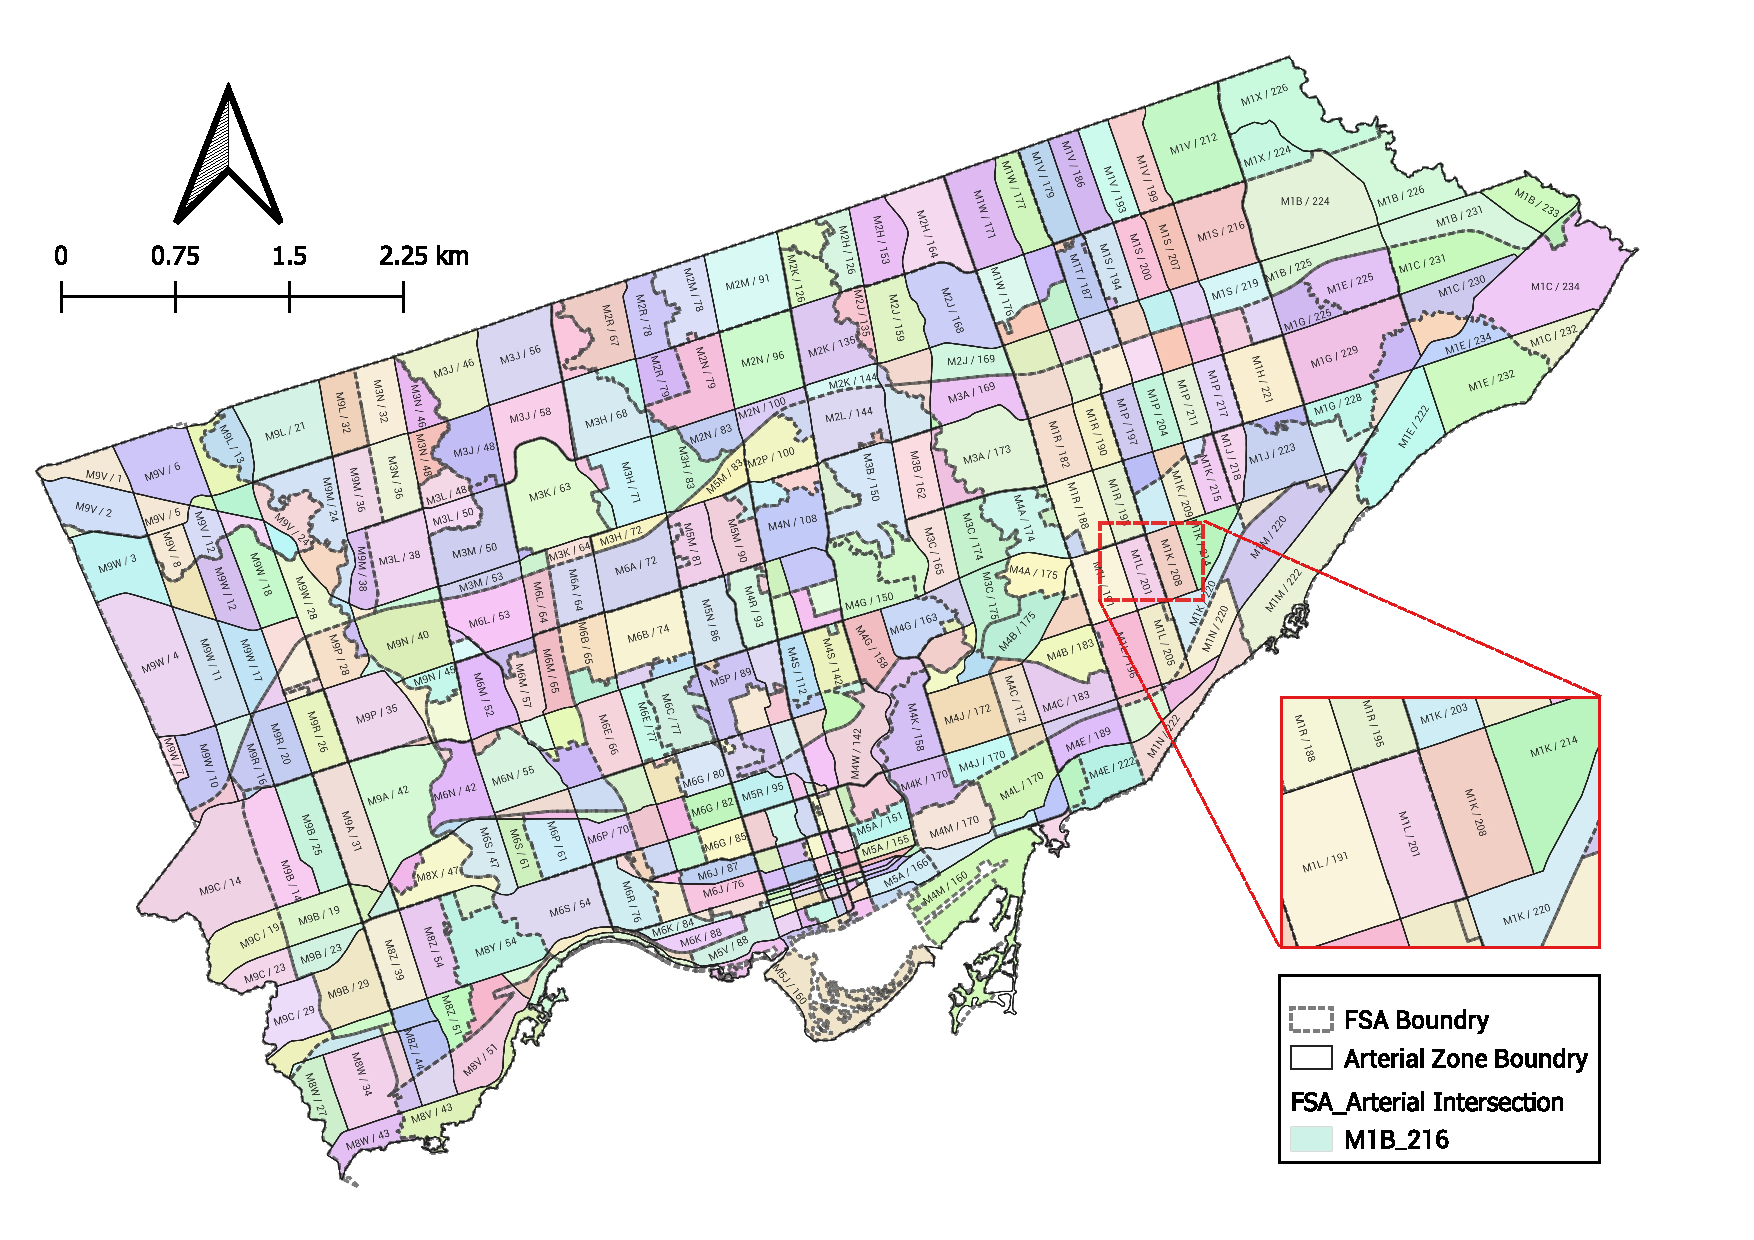
\includegraphics[width=0.7\textwidth]{images/Toronto_FSA_Arterial_intersections_JournalMap.pdf}
  \caption{Intersection between \glspl{fsa} and arterial zones for redistributing \gls{bev} ownership counts.}
  \label{fig:fsa_arterial_intersection}
\end{figure}
To recover ownership counts of \gls{bev} at the arterial scale, the allocations at each intersection are aggregated across all \glspl{fsa} that intersect each arterial zone \gls{ZArj}, as defined in Equation~\eqref{eq:EV_aggregate_arterial}.
% This aggregation step bridges the statistical domain of administrative reporting and the topological domain of arterial mobility corridors. 
It converts ownership data from the \gls{fsa} zoning schema into a spatial representation of BEV concentration defined over the arterial zoning schema, ensuring consistency with the network structure utilized in charger siting and accessibility analyses.
% While raw FSA-level data display large, discrete blocks of BEV ownership, the arterial-level representation reveals a more nuanced pattern. 
% High-density segments tend to cluster around central and midtown corridors, including Yonge Street, Bloor–Danforth, and Eglinton Avenue, corresponding to regions with greater residential and mixed-use intensity. 
% Peripheral arterial regions exhibit lower normalized densities, particularly toward Scarborough and the northwest industrial corridors, reflecting both lower residential BEV ownership and limited charging demand potential.  
% From~\eqref{eq:EV_aggregate_arterial}, and with  \gls{AAr} defined in~\eqref{eq:artertal_zones_area}, the absolute ownership counts are converted into intensity measures according to Equation~\eqref{eq:EV_density_arterial}. The resulting \gls{bev} density \gls{rhoAr} enables direct comparison of concentration levels across arterial zones of unequal size. 
% The normalization procedure~\eqref{eq:EV_density_norm} scales the densities to the unit interval, facilitating direct comparison across corridors of unequal size. 
% This enables subsequent analyses, such as charger-demand alignment, spatial equity assessment, and ridge-path demand extraction, to be performed without bias from differing region areas or total \gls{bev} counts. 
% Following normalization, a spatial smoothing procedure is applied to reduce small-area noise and account for spatial spillovers across adjacent arterial zones. As described in Equation~\eqref{eq:EV_density_nhop_weighted}, each arterial-zone \gls{bev} density is replaced by a weighted local average computed over its neighbours. The smoothing employs an $n$-hop distance structure, where the densities of neighbouring zones within $n$ steps contribute according to a convex weight vector $\mathbf{w}$. In this analysis, the hyperparameters were set to $n=1$ and $w_{1}=0.5$, assigning equal influence to each zone and its immediate neighbours. 
% This one-hop smoothing preserves local variation while attenuating random fluctuations caused by boundary effects or data irregularities. The resulting smoothed-density heatmap is shown in Figure~\ref{fig:ev_density_heatmap}; the empirical distribution is summarized by the histogram in Figure~\ref{fig:ev_density_hist} and the descriptive statistics in Table~\ref{tab:ev_density_stats}.
Absolute ownership counts are first converted into arterial-zone intensity measures, then normalized to the unit interval to enable unbiased comparison across arterial zones. The normalized densities are subsequently smoothed using a one-hop, \gls{nHop} $=1 $, weighted averaging procedure with weights $w_{0}=1$ and $w_{1}=0.5$, which mitigates local noise and boundary effects while preserving spatial variation. The resulting smoothed \gls{bev} density distribution is illustrated in Figure~\ref{fig:ev_density_heatmap}, with summary statistics reported in Figure~\ref{fig:ev_density_hist} and Table~\ref{tab:ev_density_stats}.

\begin{figure}[htbp]
  \centering
  \captionsetup{justification=centering}
  % (a) Heatmap
  \begin{subfigure}[t]{0.49\textwidth}
    \centering
    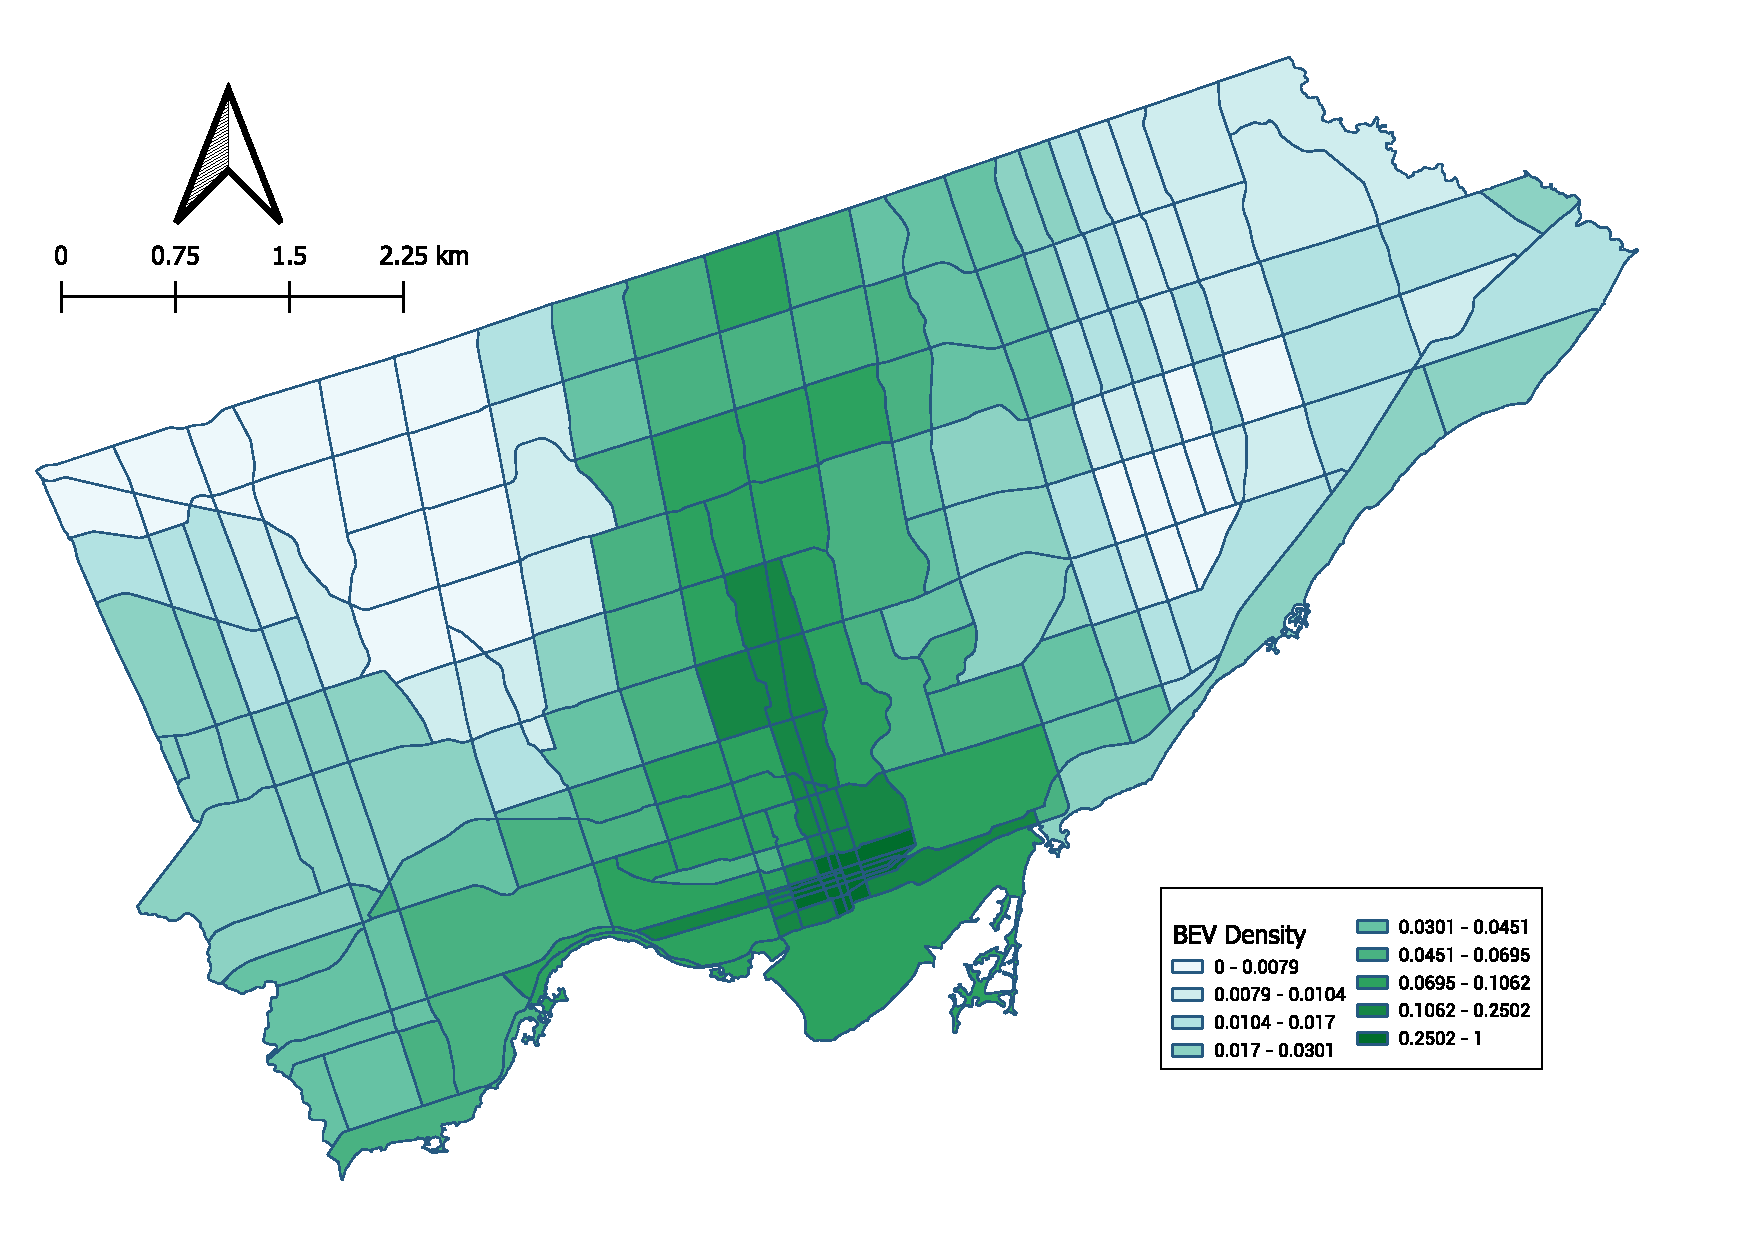
\includegraphics[width=\linewidth,
                     height=0.55\textheight,
                     keepaspectratio,
                     pagebox=cropbox]{images/Toronto_arterial_zones_BEV_densities_JournalMap.pdf}
    \caption{Smoothed \gls{bev} density heatmap across Toronto’s arterial zones. 
    Colors encode \gls{rhoArSmooth} values derived from one-hop smoothing.}
    \label{fig:ev_density_heatmap}
  \end{subfigure}\hfill
  % (b) Histogram
  \begin{subfigure}[t]{0.49\textwidth}
    \centering
    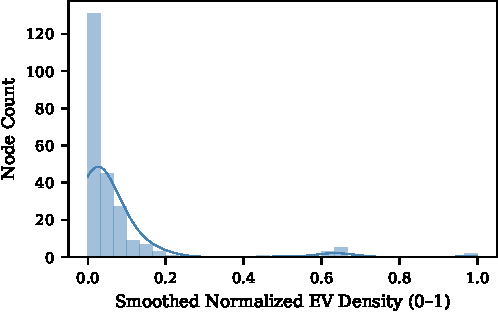
\includegraphics[width=\linewidth,
                     height=0.55\textheight,
                     keepaspectratio,
                     pagebox=cropbox]{images/ev_density_distribution.pdf}
    \caption{Histogram showing the distribution of smoothed \gls{bev} densities \gls{rhoArSmooth} across arterial zones.}
    \label{fig:ev_density_hist}
  \end{subfigure}

  \caption{Spatial and statistical representation of smoothed \gls{bev} densities across arterial zones: 
  (a) heatmap of $\tilde{\rho}^{\mathrm{Ar}}_{j}$ values; 
  (b) corresponding empirical distribution.}
  \label{fig:ev_density_visuals}
\end{figure}

% s


% The resulting distribution of $\widehat{\rho}^{\mathrm{Ar}}_{j}$ exhibits strong spatial autocorrelation (high–high clustering), consistent with corridor-continuous demand patterns rather than random dispersion.

% Overall, the derived arterial EV density layer forms a meso-level representation of ownership-driven demand potential. 
% It bridges the gap between coarse administrative data and the fine-grained spatial logic of urban mobility corridors, providing a consistent quantitative foundation for charger placement, network optimization, and equity-driven infrastructure planning.

% \begin{figure}[htbp]
%   \centering
%   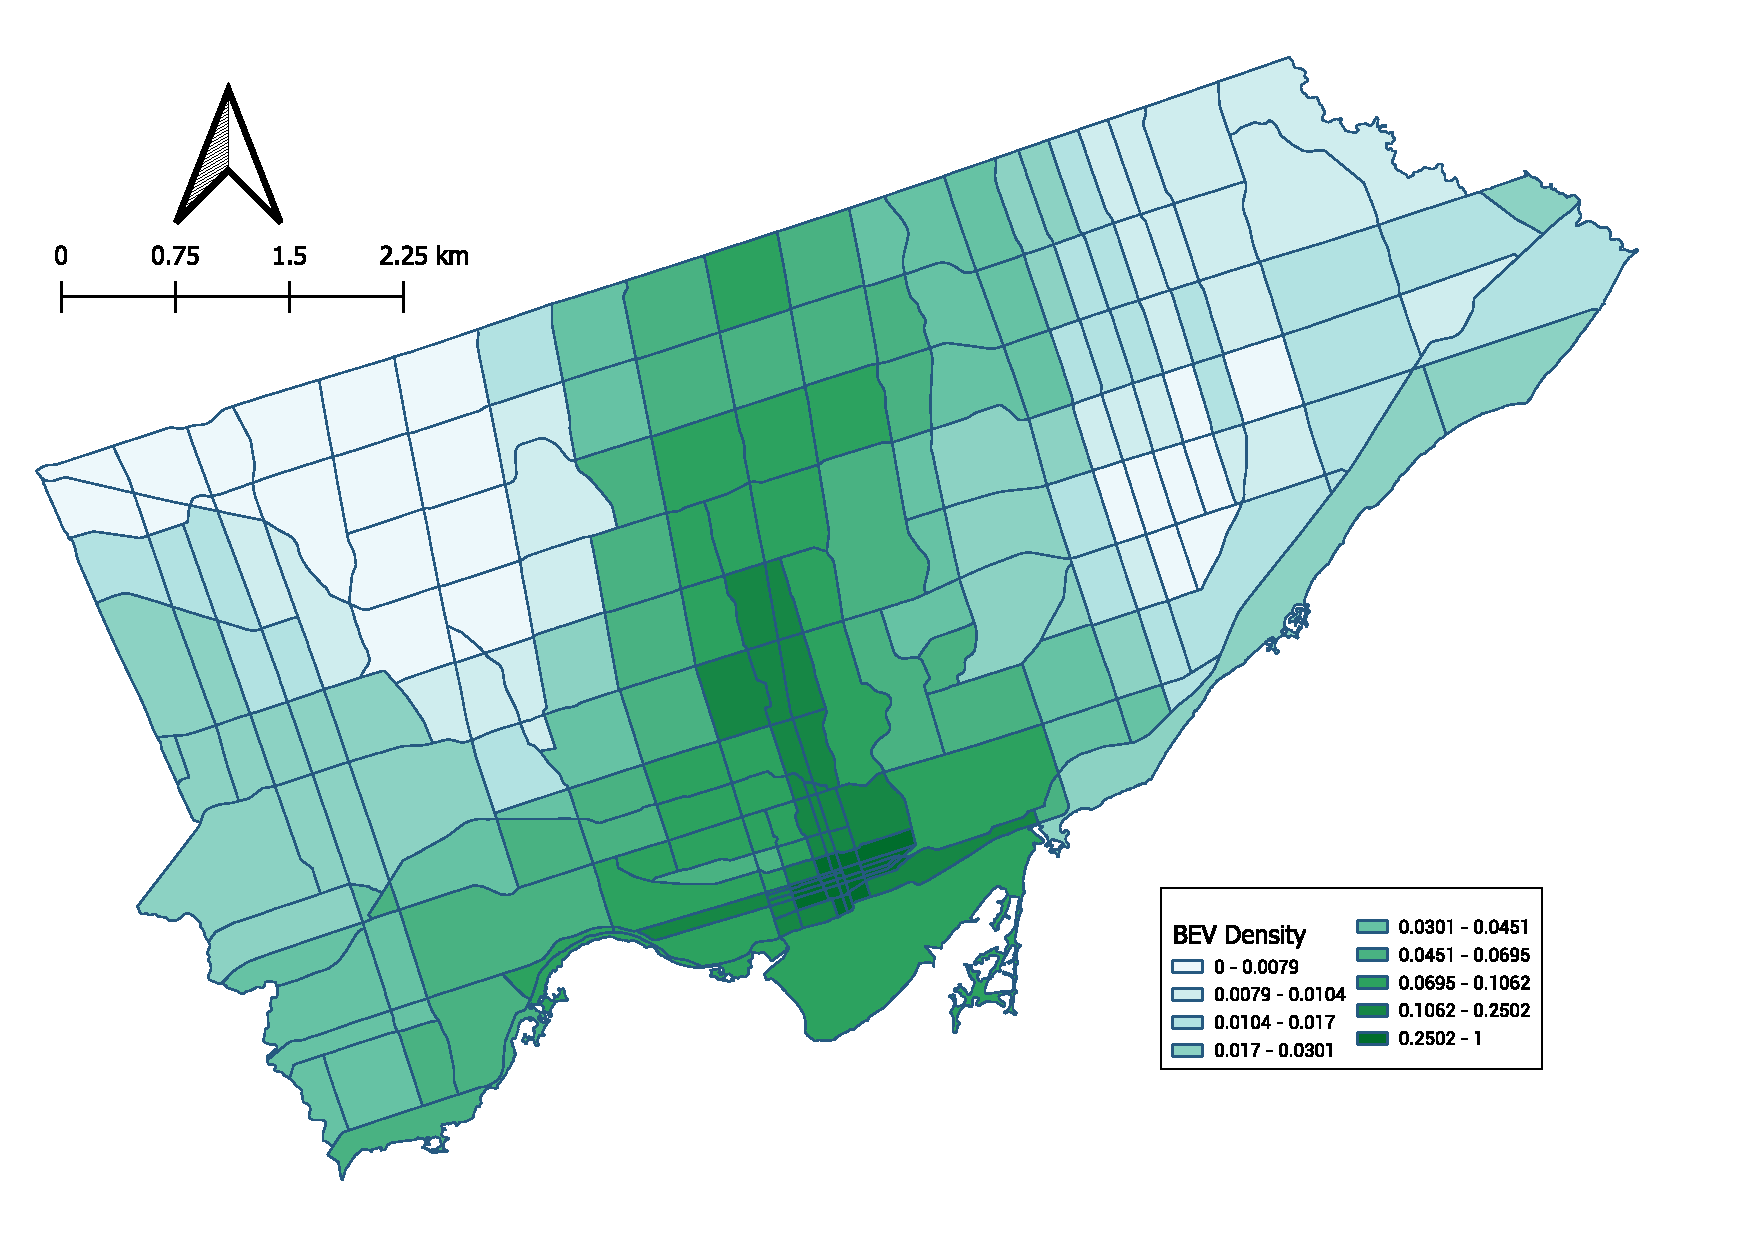
\includegraphics[width=0.9\textwidth]{images/Toronto_arterial_zones_BEV_densities_JournalMap.pdf}
%   \caption{Smoothed BEV density ($\tilde{\rho}^{\mathrm{Ar}}_{j}$) across arterial zones in the City of Toronto.}
%   \label{fig:arterial_ev_density}
% \end{figure}

% \subsection{Preprocessing and Spatial Setup}
% \label{subsec:preprocessing}
% EV counts are dasymetrically disaggregated from FSAs to intersection regions (Eq.~\eqref{eq:EV_allocation_intersection}) and aggregated to arterial zones (Eq.~\eqref{eq:EV_aggregate_arterial}), then normalized (Eq.~\eqref{eq:EV_density_norm}).
\subsection{Graph constraction}
\label{subsec:hop_distance_results}

The planar adjacency graph defined in Equation~\eqref{eq:urban_graph} yields a connected and topologically coherent representation of Toronto's arterial zones, as illustrated in Figure~\ref{fig:local_maxima_map}. 
Each vertex corresponds to the centroid of an arterial polygon, and edges connect zones that share a nonzero boundary segment. 
The resulting graph contains $|$\gls{VertexSet}$| = 234$ vertices and $|$\gls{EdgeSet}$| = 479$ undirected edges, as shown in Table~\ref{tab:graph_overview}.
% \begin{figure}[!ht]
%   \centering
%   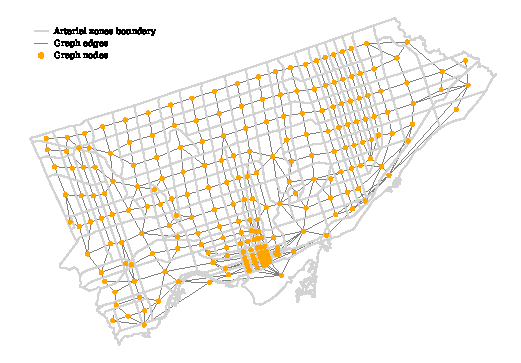
\includegraphics[width=0.85\textwidth]{images/toronto_arterial_graph.pdf}
%   \caption{Adjacency graph of Toronto's arterial zones. 
%   Nodes correspond to zone centroids and edges connect zones sharing common boundaries.}
%   \label{fig:arterial_graph}
% \end{figure}

%========================
% Graph-Theoretic Analysis
%========================
\subsubsection{Graph-theoretic analysis of the arterial adjacency network}
\label{subsec:graph_analysis}
The edge density is low $0.0176$, indicating a sparse mesh, expected for an adjacency graph rather than a road-traffic graph. Despite sparsity, the graph is fully connected, one component, ensuring network-wide reachability.
Node degrees range from $2$ to $9$, with a median of $4$ and a mean of $4.094$. No leaves are present, leaf fraction $=0$, indicating that every zone maintains at least two distinct neighbors and thus exhibits non-fragile local connectivity. The hub set is modest, with a maximum degree of $9$, ensuring that no extreme star-like structures emerge, as shown in Table~\ref{tab:top_degree}.
Global transitivity is $0.1418$ and the average local clustering is $0.1406$, with a total of $75$ triangles. This indicates a moderate level of triadic closure, meaning that some groups of three adjacent zones form closed loops. Such local triangular connections provide short alternative paths and enhance spatial redundancy, while maintaining the network’s sparse corridor structure rather than forming overly dense clusters.
% \paragraph{Connectivity and Resilience.}
The graph has no bridges and no articulation points. Hence, removing any single edge or single node does not disconnect the network. In topological terms, the network is robust to single-point failures.
% \paragraph{Core Decomposition.}
The maximum $k$-core is $k_{\max}=3$, containing $224$ nodes ($\approx 95.7\%$ of $V$). Nearly the entire network participates in a 3-core, which signals pervasive redundancy: most zones are embedded within triads and maintain degree $\ge 3$ inside the core.
% \paragraph{Path Structure.}
On the only connected component, the average shortest path length is $7.8523$, with diameter $20$ and radius $12$. The large diameter/radius indicates an elongated, corridor-like structure at the city scale: a single site cannot provide short-hop access city-wide; multi-seed strategies are mandatory.

% \paragraph{Assortativity.}
The degree assortativity coefficient is $r = 0.0789$, indicating a weakly positive correlation between the degrees of adjacent zones. This result implies that well-connected arterial zones tend to be linked slightly more frequently with other well-connected zones, whereas sparsely connected zones are more likely to border similarly sparse ones. The absence of a pronounced hub-leaf structure indicates a balanced and non-hierarchical pattern of connectivity across the arterial zones network. Greedy modularity analysis identifies $7$ distinct communities with sizes of $[52 ,45 ,42 ,41 ,30 ,17 ,7]$, as summarized in Table~\ref{tab:communities}. These communities represent coherent meso-scale clusters of arterial connectivity and provide a natural basis for decentralized planning and staged infrastructure deployment, such as assigning at least one \gls{fc} hub to each community followed by intra-community optimization.

Node \texttt{170} ranks highest across multiple centrality measures, including degree, betweenness, closeness, and eigenvector centrality, indicating its pivotal structural role within the network. Node \texttt{222} also exhibits consistently high centrality, underscoring its importance as a secondary hub. The primary betweenness hotspots, nodes \texttt{170}, \texttt{222}, \texttt{160}, \texttt{166}, \texttt{54}, \texttt{181}, \texttt{75}, \texttt{150}, \texttt{158}, and \texttt{62}, function as inter-community gateways in the modular structure of the network, as reported in Table~\ref{tab:top_betweenness}. These nodes are strategic candidates for the placement of high-capacity facilities, as they mediate flows between communities and alleviate cross-community bottlenecks. Degree alone is insufficient to characterize such nodes, since the maximum degree remains moderate; a composite interpretation integrating betweenness, closeness, and eigenvector centralities provides a more accurate delineation of the network’s functional backbone, as summarized in Tables~\ref{tab:top_closeness}--\ref{tab:top_degree_centrality}.
Collectively, the adjacency graph serves as the backbone for subsequent ridge-path analyses, enabling the integration of topological proximity into \gls{bev} activity modeling.
\subsubsection{Ridge path extraction}
\label{subsubsec:ridge_path_results}
Ridge path extraction identifies the high-density corridor zones within the arterial adjacency graph by tracing sequences of zones that consistently maintain elevated \gls{bev} densities. 
% The procedure begins by detecting the set of local maxima defined in Equation~\eqref{eq:local_maxima_set}, representing arterial zones whose smoothed densities are greater than or equal to those of all immediate neighbours. These local maxima, shown in Figure~\ref{fig:local_maxima_map}, correspond to the peaks of the smoothed \gls{bev} density surface and delineate the starting points of potential high-demand corridors. The set of local maxima zones is 
The procedure begins by identifying local maxima, corresponding to arterial zones whose smoothed densities are greater than or equal to those of all adjacent neighbours. Identified local maxima, illustrated in Figure~\ref{fig:local_maxima_map} and summarized in Table~\ref{tab:local_maxima_set_list}, represent the peaks of the smoothed \gls{bev} density surface and serve as seed nodes for initiating ridge paths.
% \begin{align}
% \label{eq:local_maxima_set_list}
% \mathcal{M} 
%   &= 
%   \{\,3,\,11,\,18,\,47,\,51,\,104,\,109,\,132,\,95,\,207,\,221,\,180,\notag\\
%   &\quad 96,\,173,\,189,\,147,\,107,\,210,\,181,\,7,\,131\,\}.
% \end{align}
% Each local maximum serves as a seed node from which a ridge path is initiated and extended according to the density-drop condition specified in Equation~\eqref{eq:ridge_path_set}.
\begin{figure}[!ht]
  \centering
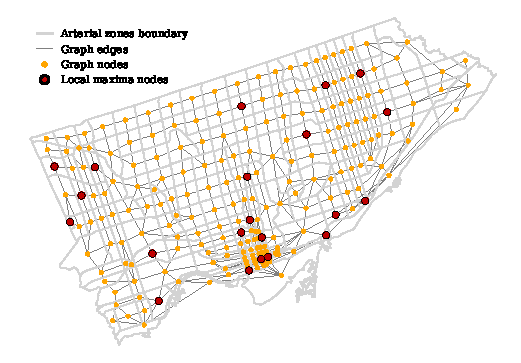
\includegraphics[width=0.7\textwidth]{images/toronto_local_maxima.pdf}
  \caption{Adjacency graph of Toronto's arterial zones, local maxima of smoothed \gls{bev} density across Toronto’s arterial zones.}
  \label{fig:local_maxima_map}
\end{figure}


Starting from each local maximum, the ridge walker, an iterative traversal algorithm, follows connected areas with a high density of \gls{bev} activity. It moves through neighboring regions where the density remains within a specified drop threshold, as outlined by the strategy-specific rules in Equations \eqref{eq:ridge_avg}-\eqref{eq:ridge_laplacian}. 
% This method allows for the continuous tracing of high-density zones from local peaks, effectively identifying the main zones of concentrated \gls{bev} activity throughout the urban network.
% The admissible set of neighbours is evaluated dynamically to ensure that the walk proceeds only along zones where densities decline gradually, preserving the continuity of high-activity zones.
Two hyperparameters govern the ridge-path extraction process: the maximum walk length \gls{L} and the drop-tolerance scaling factor \gls{eta}. The walk length is bounded by the graph diameter \gls{diamG}, set as \gls{L} $ = $ \gls{alpha}$ \times $\gls{diamG} with \gls{alpha}$ = 0.5$, limiting ridge extent to half the network span. The drop-tolerance parameter \gls{eta}$ = 0.3$ regulates the allowable descent along the density surface, smaller values enforce stricter adherence to high-density ridges, whereas larger values allow smoother, more flexible trajectories through neighbouring zones.





Five ridge-walking strategies are employed: \textsc{average}, \textsc{maximum}, \textsc{median}, \textsc{standard deviation}, and \textsc{laplacian}. Each strategy prescribes a unique rule for calculating the local drop allowance \gls{Deltat} based on the distribution of neighboring densities. These strategies offer different interpretations of ridge continuity. The \textsc{average} and \textsc{median} strategies promote balanced transitions, while the \textsc{maximum} strategy favors consistent movement along peak sequences. In contrast, the \textsc{standard deviation} and \textsc{laplacian} strategies focus on contrast-tolerant ridges that navigate through locally elevated density regions but restrict sharp declines, especially in areas with steep spatial gradients.
The minimum average density threshold \gls{rhoMin}, set at $0.0661$, corresponds to the 75th percentile of the arterial-zone density distribution, as shown in Table~\ref{tab:ev_density_stats}. This criterion ensures that only statistically significant high-density corridor zones are included.
The ridge paths extracted are visualized in Figure~\ref{fig:strategy-ridges-grid}, with each line depicting a continuous chain of arterial zones that form a corridor of high \gls{bev} activity zones.
\begin{figure*}[t]
  \centering
  % -------- Row 1: 3 panels --------
  \begin{subfigure}[t]{0.32\textwidth}
    \centering
    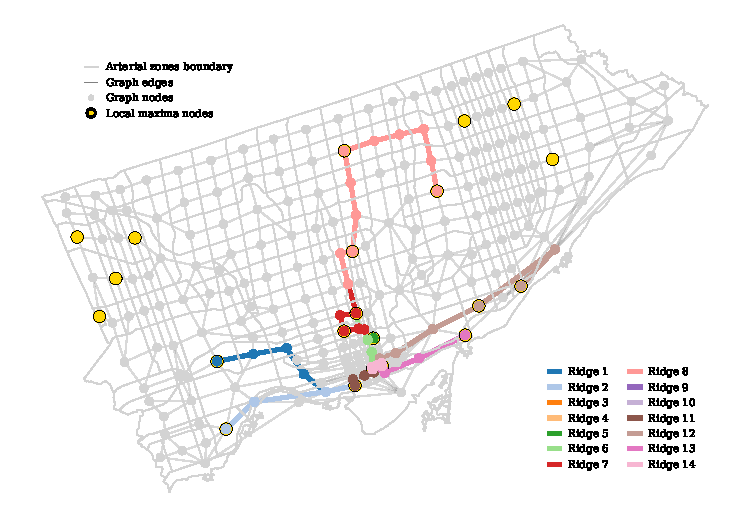
\includegraphics[width=\linewidth]{images/strategy_ridges_avg_all.pdf}
    \subcaption{Average-based ridge extraction.}
    \label{fig:ridges-avg}
  \end{subfigure}\hfill
  \begin{subfigure}[t]{0.32\textwidth}
    \centering
    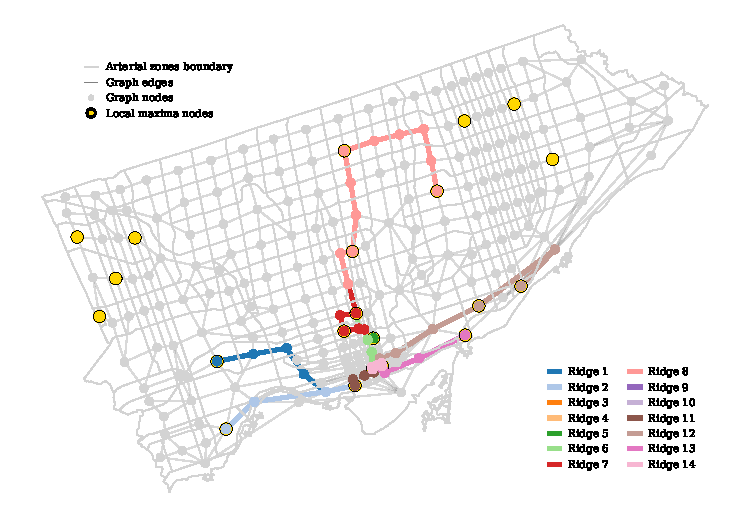
\includegraphics[width=\linewidth]{images/strategy_ridges_max_all.pdf}
    \subcaption{Maximum-based ridge extraction.}
    \label{fig:ridges-max}
  \end{subfigure}\hfill
  \begin{subfigure}[t]{0.32\textwidth}
    \centering
    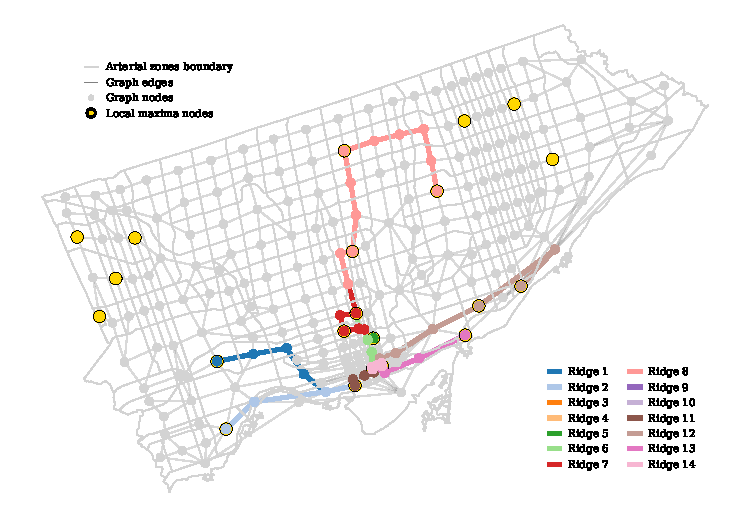
\includegraphics[width=\linewidth]{images/strategy_ridges_median_all.pdf}
    \subcaption{Median-based ridge extraction.}
    \label{fig:ridges-median}
  \end{subfigure}

  \vspace{0.6em}

  % -------- Row 2: 3 panels --------
  \begin{subfigure}[t]{0.32\textwidth}
    \centering
    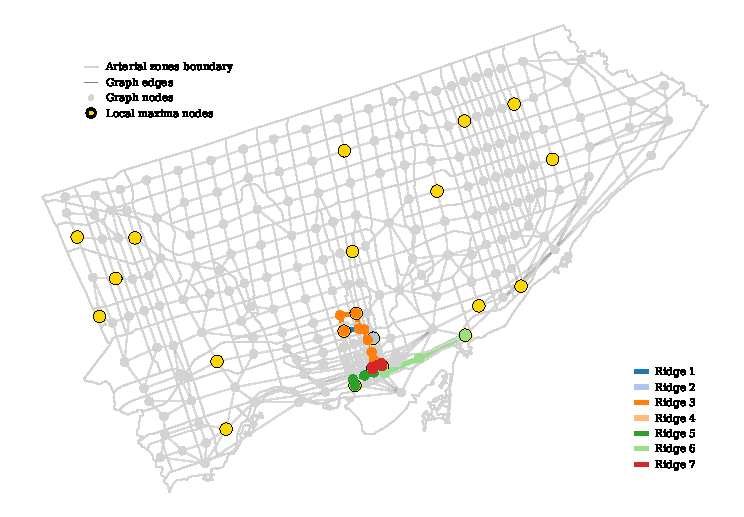
\includegraphics[width=\linewidth]{images/strategy_ridges_std_all.pdf}
    \subcaption{Standard-deviation–based ridge extraction.}
    \label{fig:ridges-std}
  \end{subfigure}\hfill
  \begin{subfigure}[t]{0.32\textwidth}
    \centering
    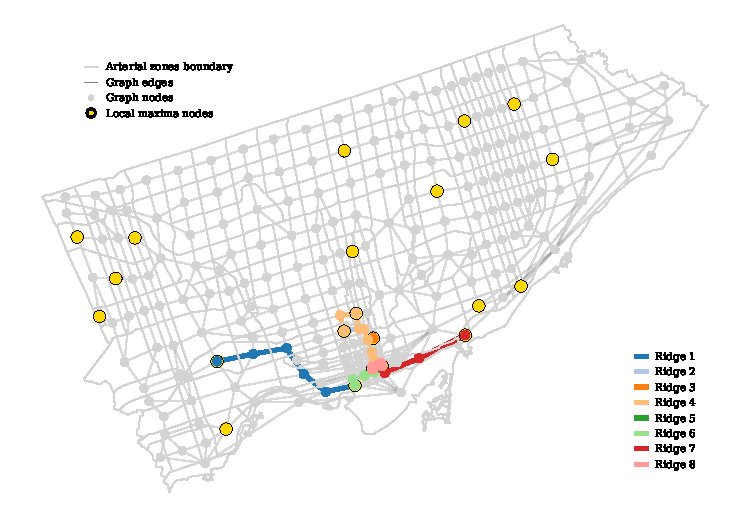
\includegraphics[width=\linewidth]{images/strategy_ridges_laplacian_all.pdf}
    \subcaption{Laplacian-based ridge extraction.}
    \label{fig:ridges-laplacian}
  \end{subfigure}\hfill
  \begin{subfigure}[t]{0.32\textwidth}
    \centering
    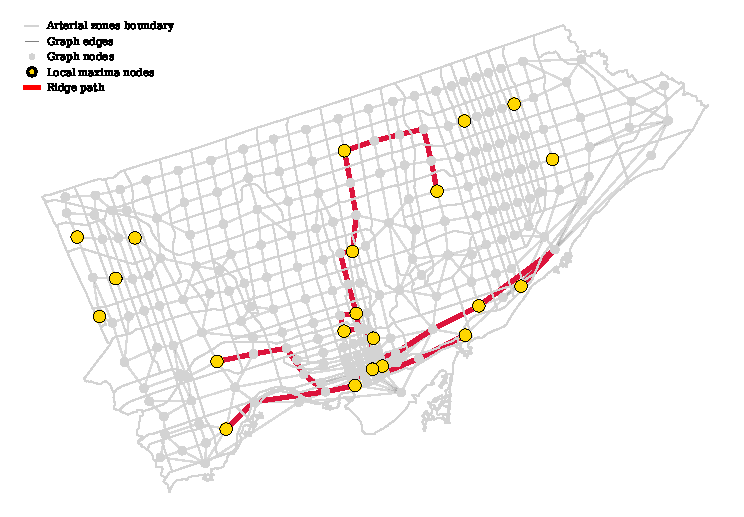
\includegraphics[width=\linewidth]{images/ridges_all_strategies_overlay_same_color.pdf}
    \subcaption{Overlay of all strategies (same ridge color).}
    \label{fig:ridges-overlay}
  \end{subfigure}

  \caption{
  Ridge-path results 
  (a) Average-based ridges; 
  (b) Maximum-based ridges; 
  (c) Median-based ridges; 
  (d) Standard-deviation–based ridges; 
  (e) Laplacian-based ridges; 
  (f) Overlay of all strategies' ridge paths drawn in a single ridge color for visual comparison.
  }
  \label{fig:strategy-ridges-grid}
\end{figure*}
\noindent
The outcomes of the ridge-path statistics for all strategies are summarized in Table~\ref{tab:ridge_summary}. The results reveal distinct behavioral patterns across the five ridge-walking strategies. The \textsc{average}, \textsc{maximum}, and \textsc{median} methods yield highly consistent ridge configurations, indicating that ridge extraction remains stable across the central-tendency formulations of the underlying \gls{bev}-density field. In contrast, the \textsc{standard deviation} and \textsc{laplacian} strategies, which are sensitive to dispersion and local contrast, produce fewer but more concentrated ridges. These methods highlight high-intensity corridors while filtering out weaker peripheral structures. Overall, central-tendency strategies favor broader coverage of regions with moderate to high density, whereas contrast-based methods delineate sharper, more dominant pathways that align with the city’s primary arterial framework.
% The results show that the average, maximum, and median strategies produce the same set of ridge paths, as illustrated in Figures~\ref{fig:ridges-avg}, \ref{fig:ridges-max}, and \ref{fig:ridges-median}, respectively. This consistency suggests that ridge extraction is reliable regardless of the central-tendency operator used for the underlying BEV-density signal. For these three strategies, each with  14  ridge paths, the mean ridge density, calculated as the average of the zone densities along each ridge path, is 0.397, while the median is 0.345. The ridge density values range from 0.078 to 1.000.
% In contrast, the \textsc{std} and \textsc{laplacian} strategies generate fewer ridge paths but with higher densities, as illustrated in Figures~\ref{fig:ridges-std} and \ref{fig:ridges-laplacian}, respectively. The \textsc{std} method produces 7 ridges with a mean of 0.559 and a median of 0.493. Meanwhile, the \textsc{laplacian} method results in 8 ridges with a mean of 0.521 and a median of 0.481, as summarized in Table~\ref{tab:ridge_summary}.
% These patterns imply that dispersion- and contrast-sensitive strategies preferentially retain persistent, high-intensity corridor zones, whereas central-tendency criteria enumerate a broader set that also includes moderate-intensity segments. 
% The \textsc{average}, \textsc{max}, and \textsc{median} methods yield the most stable ridge sets, balancing length and density preservation, whereas the \textsc{std} and \textsc{laplacian} strategies produce fewer yet higher-density, often more elongated ridges concentrated along dominant urban corridors.
% Notably, all strategies include the short, high-intensity link $147, 146$ (density $=1.000$), marking a consistent core corridor zones across strategies. 
The union of all ridge-path nodes, as defined in Equation~\eqref{eq:ridge_path_nodes}, represents the full set of arterial zones that support the mobility-based \gls{bev} activity structure, as illustrated in Figure~\ref{fig:ridges-overlay}.
% \begin{table}[htbp]
% \centering
% \caption{Extracted Ridge Nodes and Corresponding Normalized BEV Densities}
% \label{tab:ridge_ev_density}
% \setlength{\tabcolsep}{6pt}%
% \begin{minipage}[t]{0.32\linewidth}
% \vspace{0pt}%
% \centering
% \begin{tabularx}{\linewidth}{>{\centering\arraybackslash}X>{\centering\arraybackslash}X}
% \toprule
% \textbf{Node ID} & \textbf{BEV Density} \\
% \midrule
% 100 & 0.0662 \\
% 104 & 0.1067 \\
% 105 & 0.1246 \\
% 107 & 0.1263 \\
% 108 & 0.0626 \\
% 109 & 0.0996 \\
% 111 & 0.0995 \\
% 118 & 0.0960 \\
% 119 & 0.1982 \\
% 124 & 0.1405 \\
% 129 & 0.1634 \\
% 130 & 0.6356 \\
% 131 & 0.6363 \\
% 132 & 0.1470 \\
% 133 & 0.6354 \\
% 134 & 0.1658 \\
% 135 & 0.0510 \\
% 136 & 0.6311 \\
% 137 & 0.6441 \\
% 143 & 0.1280 \\
% \bottomrule
% \end{tabularx}
% \end{minipage}\hfill
% %
% \begin{minipage}[t]{0.32\linewidth}
% \vspace{0pt}%
% \centering
% \begin{tabularx}{\linewidth}{>{\centering\arraybackslash}X>{\centering\arraybackslash}X}
% \toprule
% \textbf{Node ID} & \textbf{BEV Density} \\
% \midrule
% 146 & 0.9993 \\
% 147 & 1.0000 \\
% 148 & 0.4549 \\
% 149 & 0.2031 \\
% 155 & 0.0820 \\
% 159 & 0.0432 \\
% 166 & 0.0562 \\
% 168 & 0.0433 \\
% 169 & 0.0462 \\
% 170 & 0.0447 \\
% 173 & 0.0474 \\
% 181 & 0.0597 \\
% 189 & 0.0603 \\
% 210 & 0.0205 \\
% 222 & 0.0199 \\
% 47  & 0.0567 \\
% 51  & 0.0471 \\
% 61  & 0.0513 \\
% 62  & 0.0458 \\
% 70  & 0.0482 \\
% \bottomrule
% \end{tabularx}
% \end{minipage}\hfill
% %
% \begin{minipage}[t]{0.32\linewidth}
% \vspace{0pt}%
% \centering
% \begin{tabularx}{\linewidth}{>{\centering\arraybackslash}X>{\centering\arraybackslash}X}
% \toprule
% \textbf{Node ID} & \textbf{BEV Density} \\
% \midrule
% 76  & 0.0710 \\
% 88  & 0.0968 \\
% 92  & 0.0995 \\
% 93  & 0.0995 \\
% 95  & 0.1005 \\
% 96  & 0.0873 \\
% 98  & 0.0922 \\
% \bottomrule
% \end{tabularx}
% \end{minipage}
% \end{table}



\begin{table}[!ht]
\centering
\caption{Summary of ridge-path density statistics by extraction strategy.}
\label{tab:ridge_summary}
\resizebox{\linewidth}{!}{%
\begin{tabular}{lcccccc}
\toprule
\textbf{Strategy} & \textbf{Number of Ridges} & \textbf{Mean} & \textbf{Median} & \textbf{Min} & \textbf{Max} & \textbf{Std}  \\
\midrule
\textsc{average}   & 14 & 0.397 & 0.345 & 0.078 & 1.000 & 0.249  \\
\textsc{max}       & 14 & 0.397 & 0.345 & 0.078 & 1.000 & 0.249  \\
\textsc{median}    & 14 & 0.397 & 0.345 & 0.078 & 1.000 & 0.249  \\
\textsc{std}       &  7 & 0.559 & 0.493 & 0.302 & 1.000 & 0.236  \\
\textsc{laplacian} &  8 & 0.521 & 0.481 & 0.252 & 1.000 & 0.243 \\
\bottomrule
\end{tabular}%
}
% \vspace{0.25em}

\end{table}

% \begin{table}[!ht]
% \centering
% \caption{Extracted ridge paths using the \textsc{average} strategy.}
% \label{tab:ridge_avg}
% \resizebox{\linewidth}{!}{%
% \begin{tabular}{ccc}
% \toprule
% \textbf{Ridge ID} & \textbf{Avg. Density} & \textbf{Node Sequence} \\
% \midrule
% 1 & 0.252 & 47→61→70→76→88→107→105→119→133→131→130 \\
% 2 & 0.388 & 51→62→88→107→105→119→133→131→130→137→146 \\
% 3 & 0.125 & 104→93→98→109→92→95→111→118→124→129→134 \\
% 4 & 0.302 & 109→92→95→111→118→124→129→134→136→137→146 \\
% 5 & 0.493 & 132→124→129→134→136→137→146→147 \\
% 6 & 0.302 & 95→92→109→111→118→124→129→134→136→137→146 \\
% 7 & 0.102 & 96→100→108→104→93→98→109→92→95→111→118 \\
% 8 & 0.078 & 173→169→168→159→135→96→100→108→104→93→98 \\
% 9 & 0.393 & 189→170→155→143→146→147 \\
% 10 & 1.000 & 147→146 \\
% 11 & 0.561 & 107→105→119→133→131→130→137→146→147 \\
% 12 & 0.302 & 210→222→189→170→155→143→146→147 \\
% 13 & 0.469 & 181→166→149→148→147→146 \\
% 14 & 0.786 & 131→130→137→146→147 \\
% \bottomrule
% \end{tabular}%
% }
% \end{table}

% \begin{table}[!ht]
% \centering
% \caption{Ridge paths extracted using the \textsc{max} strategy.}
% \label{tab:ridge_max}
% \resizebox{\linewidth}{!}{%
% \begin{tabular}{ccc}
% \toprule
% \textbf{Ridge ID} & \textbf{Avg. Density} & \textbf{Node Sequence} \\
% \midrule
% 1 & 0.252 & 47→61→70→76→88→107→105→119→133→131→130 \\
% 2 & 0.388 & 51→62→88→107→105→119→133→131→130→137→146 \\
% 3 & 0.125 & 104→93→98→109→92→95→111→118→124→129→134 \\
% 4 & 0.302 & 109→92→95→111→118→124→129→134→136→137→146 \\
% 5 & 0.493 & 132→124→129→134→136→137→146→147 \\
% 6 & 0.302 & 95→92→109→111→118→124→129→134→136→137→146 \\
% 7 & 0.102 & 96→100→108→104→93→98→109→92→95→111→118 \\
% 8 & 0.078 & 173→169→168→159→135→96→100→108→104→93→98 \\
% 9 & 0.393 & 189→170→155→143→146→147 \\
% 10 & 1.000 & 147→146 \\
% 11 & 0.561 & 107→105→119→133→131→130→137→146→147 \\
% 12 & 0.302 & 210→222→189→170→155→143→146→147 \\
% 13 & 0.469 & 181→166→149→148→147→146 \\
% 14 & 0.786 & 131→130→137→146→147 \\
% \bottomrule
% \end{tabular}%
% }
% \end{table}

% \begin{table}[!ht]
% \centering
% \caption{Ridge paths extracted using the \textsc{median} strategy.}
% \label{tab:ridge_median}
% \resizebox{\linewidth}{!}{%
% \begin{tabular}{ccc}
% \toprule
% \textbf{Ridge ID} & \textbf{Avg. Density} & \textbf{Node Sequence} \\
% \midrule
% 1 & 0.252 & 47→61→70→76→88→107→105→119→133→131→130 \\
% 2 & 0.388 & 51→62→88→107→105→119→133→131→130→137→146 \\
% 3 & 0.125 & 104→93→98→109→92→95→111→118→124→129→134 \\
% 4 & 0.302 & 109→92→95→111→118→124→129→134→136→137→146 \\
% 5 & 0.493 & 132→124→129→134→136→137→146→147 \\
% 6 & 0.302 & 95→92→109→111→118→124→129→134→136→137→146 \\
% 7 & 0.102 & 96→100→108→104→93→98→109→92→95→111→118 \\
% 8 & 0.078 & 173→169→168→159→135→96→100→108→104→93→98 \\
% 9 & 0.393 & 189→170→155→143→146→147 \\
% 10 & 1.000 & 147→146 \\
% 11 & 0.561 & 107→105→119→133→131→130→137→146→147 \\
% 12 & 0.302 & 210→222→189→170→155→143→146→147 \\
% 13 & 0.469 & 181→166→149→148→147→146 \\
% 14 & 0.786 & 131→130→137→146→147 \\
% \bottomrule
% \end{tabular}%
% }
% \end{table}

% \begin{table}[!ht]
% \centering
% \caption{Ridge paths extracted using the \textsc{std} strategy.}
% \label{tab:ridge_std}
% \resizebox{\linewidth}{!}{%
% \begin{tabular}{ccc}
% \toprule
% \textbf{Ridge ID} & \textbf{Avg. Density} & \textbf{Node Sequence} \\
% \midrule
% 1 & 0.302 & 109→92→95→111→118→124→129→134→136→137→146 \\
% 2 & 0.493 & 132→124→129→134→136→137→146→147 \\
% 3 & 0.302 & 95→92→109→111→118→124→129→134→136→137→146 \\
% 4 & 1.000 & 147→146 \\
% 5 & 0.561 & 107→105→119→133→131→130→137→146→147 \\
% 6 & 0.469 & 181→166→149→148→147→146 \\
% 7 & 0.786 & 131→130→137→146→147 \\
% \bottomrule
% \end{tabular}%
% }
% \end{table}

% \begin{table}[!ht]
% \centering
% \caption{Ridge paths extracted using the \textsc{laplacian} strategy.}
% \label{tab:ridge_laplacian}
% \resizebox{\linewidth}{!}{%
% \begin{tabular}{ccc}
% \toprule
% \textbf{Ridge ID} & \textbf{Avg. Density} & \textbf{Node Sequence} \\
% \midrule
% 1 & 0.252 & 47→61→70→76→88→107→105→119→133→131→130 \\
% 2 & 0.302 & 109→92→95→111→118→124→129→134→136→137→146 \\
% 3 & 0.493 & 132→124→129→134→136→137→146→147 \\
% 4 & 0.302 & 95→92→109→111→118→124→129→134→136→137→146 \\
% 5 & 1.000 & 147→146 \\
% 6 & 0.561 & 107→105→119→133→131→130→137→146→147 \\
% 7 & 0.469 & 181→166→149→148→147→146 \\
% 8 & 0.786 & 131→130→137→146→147 \\
% \bottomrule
% \end{tabular}%
% }
% \end{table}
% The ridge-path extraction framework highlights the hierarchical organization of \gls{bev} activity across arterial zones. High-activity ridges indicate the core areas of the urban \gls{bev} ecosystem, where the deployment of charging infrastructure is anticipated to have the greatest impact on vehicle utilization.
\subsection{Proximity analysis between ridge zones and the \gls{dcfc} network}
\label{subsec:results_wpd}
\noindent The graph-based proximity analysis assesses the spatial accessibility between \gls{bev} activities along arterial ridge paths and the existing FLO \gls{dcfc} network. Table~\ref{tab:flo_dcfc_full} summarizes the technical characteristics of the FLO \gls{dcfc} stations, while Figure~\ref{fig:flo_dcfc_map}  illustrates their spatial distribution throughout Toronto's arterial network. The \gls{wpd} metric is then applied to evaluate how effectively the charging supply nodes serve the ridge-path nodes within the arterial-zone graph. 
% Together, these visual and tabular summaries provide the empirical basis for subsequent proximity-based accessibility and network-alignment evaluations.
\begin{figure}[htbp]
  \centering
  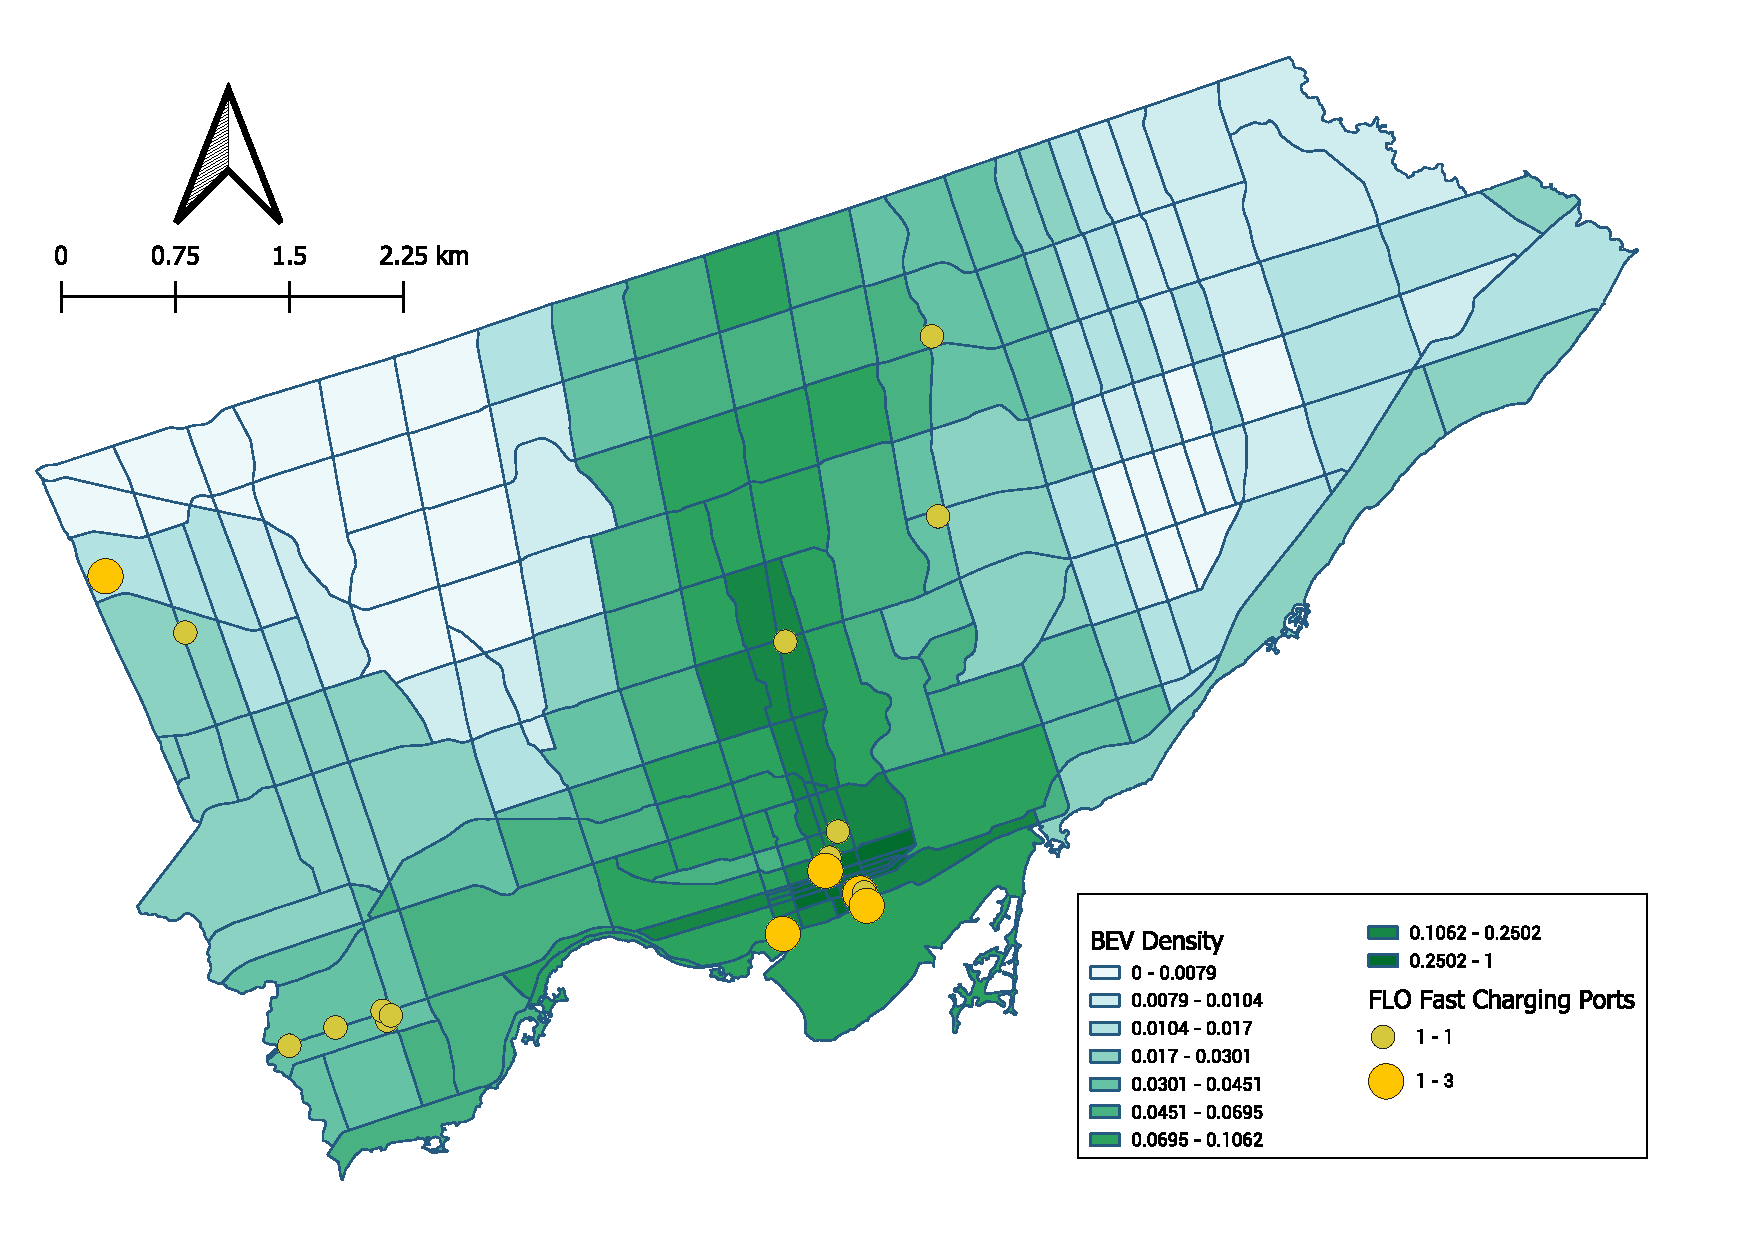
\includegraphics[width=0.7\textwidth]{images/Toronto_FLO_fastcharging_network_JournalMap.pdf}
  \caption{Spatial distribution of FLO \gls{dcfc} stations across Toronto. 
  Each point represents a station, scaled by its aggregate charging capacity (kW).}
  \label{fig:flo_dcfc_map}
\end{figure}
% \begin{table}[htbp]
% \centering
% \caption{FLO DCFC Stations in Toronto}
% \label{tab:flo_dcfc_full}
% \resizebox{\textwidth}{!}{%
% \begin{tabular}{lrrrrr}
% \toprule
% \textbf{Station Name} & \textbf{Latitude} & \textbf{Longitude} & \textbf{DC Ports} & \textbf{Per-Port (kW)} & \textbf{Station (kW)} \\
% \midrule
% Cadillac Fairview - Sherway Gardens & 43.61297 & -79.56000 & 1 & 100 & 100 \\
% Canadian Tire - Etobicoke & 43.61711 & -79.54490 & 1 & 100 & 100 \\
%  Cadillac Fairview - Shops at Don Mills & 43.73530 & -79.34550 & 1 & 100 & 100 \\
% Cadillac Fairview - Fairview Mall & 43.77787 & -79.34630 & 1 & 100 & 100 \\
% Cadillac Fairview - Toronto Eaton Centre & 43.65507 & -79.38310 & 1 & 100 & 100 \\
% 110 Queen St W.& 43.65201 & -79.38450 & 3 & 100 & 300 \\
% AURA Lake Shore BLVD & 43.63729 & -79.39870 & 2 & 100 & 200 \\
% Woodbine Nissan& 43.71108 & -79.59150 & 1 & 100 & 100 \\
% AURA Humberwood & 43.72472 & -79.61720 & 2 & 100 & 200 \\
% 2 Church St& 43.64648 & -79.37330 & 3 & 100 & 300 \\
% CP29 - 75 Holly St - Fast Charger & 43.70635 & -79.39610 & 1 & 100 & 100 \\
% 2 Church St - Fast Charger East & 43.64676 & -79.37190 & 1 & 100 & 100 \\
% 100 Queens Quay East& 43.64356 & -79.37120 & 2 & 100 & 200 \\
% Marino’s Fine Cars Subaru& 43.61852 & -79.52800 & 1 & 100 & 100 \\
% Volvo Cars Metro West& 43.62084 & -79.52940 & 1 & 100 & 100 \\
% Honda Queensway - DC & 43.61976 & -79.52680 & 1 & 100 & 100 \\
% Lexington Condominiums South Side & 43.66123 & -79.38020 & 1 & 100 & 100 \\
% \bottomrule
% \end{tabular}%
% }
% \end{table}
FLO \gls{dcfc} stations were mapped to the arterial zones. This mapping allowed for the aggregation of charging capacity and the number of sites at the zone level. As summarized in Table~\ref{tab:charger_region_summary}, thirteen arterial zones across Toronto each host at least one FLO DCFC installation, with the number of ports per zone ranging from one to four.

% \begin{table}[htbp]
% \centering
% \footnotesize
% \caption{Mapped FLO \gls{dcfc} Network Across Arterial Regions}
% \label{tab:charger_region_summary}
% \begin{tabularx}{\linewidth}{lccc}
% \toprule
% \textbf{Region ID} & \textbf{Total ports} & \textbf{Number of sites} & \textbf{Avg. ports per site} \\
% \midrule
% 107 & 2 & 1 & 2.0 \\
% 11  & 1 & 1 & 1.0 \\
% 112 & 1 & 1 & 1.0 \\
% 127 & 3 & 1 & 3.0 \\
% 134 & 1 & 1 & 1.0 \\
% 140 & 1 & 1 & 1.0 \\
% 149 & 4 & 2 & 2.0 \\
% 160 & 2 & 1 & 2.0 \\
% 165 & 1 & 1 & 1.0 \\
% 168 & 1 & 1 & 1.0 \\
% 29  & 2 & 2 & 1.0 \\
% 3   & 2 & 1 & 2.0 \\
% 30  & 3 & 3 & 1.0 \\
% \bottomrule
% \end{tabularx}
% \end{table}
% Across all ridge paths extracted in Section~\ref{sec:derived_AZ}, the mean WPD value is $1.9419$~hops, indicating that the average high-demand corridor zones are separated by approximately two to three intermediate zones from its nearest fast charger, as summarized in Table~\ref{tab:ridge_hop_distance}.
% \begin{table}[htbp]
% \centering
% \caption{Hop Distance to Nearest Charger for Ridge Nodes (three-part view)}
% \label{tab:ridge_hop_distance}
% \setlength{\tabcolsep}{6pt}%
% \begin{minipage}[t]{0.32\linewidth}
% \vspace{0pt}%
% \centering
% \begin{tabularx}{\linewidth}{>{\raggedright\arraybackslash}X>{\centering\arraybackslash}X}
% \toprule
% \textbf{Node ID} & \textbf{Hop Dist.} \\
% \midrule
% 100 & 5 \\
% 104 & 3 \\
% 105 & 0 \\
% 107 & 1 \\
% 108 & 4 \\
% 109 & 2 \\
% 111 & 1 \\
% 118 & 1 \\
% 119 & 1 \\
% 124 & 0 \\
% 129 & 1 \\
% 130 & 4 \\
% 131 & 3 \\
% 132 & 0 \\
% 133 & 2 \\
% 134 & 2 \\
% 135 & 6 \\
% 136 & 3 \\
% 137 & 4 \\
% 143 & 2 \\
% \bottomrule
% \end{tabularx}
% \end{minipage}\hfill
% %
% \begin{minipage}[t]{0.32\linewidth}
% \vspace{0pt}%
% \centering
% \begin{tabularx}{\linewidth}{>{\raggedright\arraybackslash}X>{\centering\arraybackslash}X}
% \toprule
% \textbf{Node ID} & \textbf{Hop Dist.} \\
% \midrule
% 146 & 3 \\
% 147 & 4 \\
% 148 & 4 \\
% 149 & 3 \\
% 155 & 2 \\
% 159 & 6 \\
% 166 & 3 \\
% 168 & 5 \\
% 169 & 6 \\
% 170 & 2 \\
% 173 & 5 \\
% 181 & 3 \\
% 189 & 3 \\
% 210 & 1 \\
% 222 & 2 \\
% 47  & 3 \\
% 51  & 1 \\
% 61  & 2 \\
% 62  & 2 \\
% 70  & 1 \\
% \bottomrule
% \end{tabularx}
% \end{minipage}\hfill
% %
% \begin{minipage}[t]{0.32\linewidth}
% \vspace{0pt}%
% \centering
% \begin{tabularx}{\linewidth}{>{\raggedright\arraybackslash}X>{\centering\arraybackslash}X}
% \toprule
% \textbf{Node ID} & \textbf{Hop Dist.} \\
% \midrule
% 76  & 2 \\
% 88  & 1 \\
% 92  & 1 \\
% 93  & 4 \\
% 95  & 0 \\
% 96  & 5 \\
% 98  & 3 \\
% 159 & 6 \\
% 166 & 3 \\
% 168 & 5 \\
% 169 & 6 \\
% 170 & 2 \\
% 173 & 5 \\
% 181 & 3 \\
% 189 & 3 \\
% 210 & 1 \\
% 222 & 2 \\
% \bottomrule
% \end{tabularx}
% \end{minipage}
% \end{table}
% When demand nodes are weighted by normalized BEV density $\widehat{\rho}^{\mathrm{Ar}}_j$ and charger zones by normalized supply capacity $\widehat{\rho}^{\mathrm{Ch}}_j$, accessibility improves within the downtown and central arterial corridors but degrades markedly toward the periphery.  
% Figure~\ref{fig:wpd_map} illustrates the spatial pattern of hop-based accessibility, highlighting clusters of well-served ridges along major arterials (e.g., Yonge Street, Bloor Street, and the Gardiner corridor) and extended underserved chains along the outer arterial belt.
% \paragraph{Spatial correlation between demand and supply.}
% Figure~\ref{fig:demand_supply_scatter} compares normalized charger capacity density $\widehat{\rho}^{\mathrm{Ch}}_j$ with normalized BEV density $\widehat{\rho}^{\mathrm{Ar}}_j$ across all arterial zones.  
% A moderate positive correlation ($r = 0.47$) suggests that fast chargers are preferentially located in zones with higher BEV activity, although substantial scatter remains, particularly across mid-density arterial corridors where charger deployment lags behind demand.  
% Notably, several ridge nodes exhibit $\widehat{\rho}^{\mathrm{Ar}}_j > 0.8$ yet are separated by more than three hops from the nearest high-capacity charger, revealing potential accessibility gaps.
To establish the null distribution as a baseline for evaluating proximity alignment, we first conducted an elbow analysis to determine the minimum number of random realizations needed for convergence. As shown in Figure~\ref{fig:elbow_plot}, the average value of \gls{wpd}, represented as \gls{muR}, stabilized after approximately 100 simulations. This indicated that the null distribution had reached statistical equilibrium. 
The locations of the chargers were randomized 1,050 times within the arterial-zone framework, while maintaining the empirical distribution of charging capacities. The larger number of realizations was chosen to ensure a sufficiently extensive sampling space for robust estimation of tail probabilities and to improve the statistical precision of the baseline distribution.
% This convergence threshold ensures that the null model $\mathcal{M}0$ adequately captures the random spatial variability of unconstrained charger placement while maintaining computational efficiency.
% Accordingly, $R = 1{,}050$ simulations were executed to construct the final null distribution, providing a robust reference against which the observed network could be evaluated.
% PGFPlots figure (Elsevier-friendly, 12pt). Requires \usepackage{pgfplots} and \pgfplotsset{compat=1.18}
% Requires: \usepackage{pgfplots} \pgfplotsset{compat=1.18}
\begin{figure}[htbp]
  \centering
  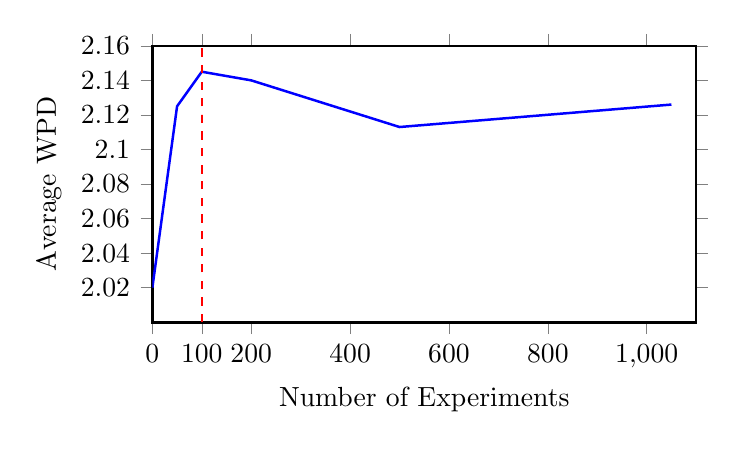
\begin{tikzpicture}
    \begin{axis}[
      width=0.7\textwidth,
      height=0.42\textwidth,
      xlabel={Number of Experiments},
      ylabel={Average WPD},
      xmin=0, xmax=1100,
      xtick={0,100,200,400,600,800,1000},
      ymin=2.00, ymax=2.16,
      ytick={2.02,2.04,2.06,2.08,2.10,2.12,2.14,2.16},
      tick align=outside,
      % grid=both,
      % grid style={line width=.2pt, draw=gray!30},
      line width=0.9pt,
      mark size=2pt
    ]
      \addplot+[mark=none] table[row sep=\\]{
        x   y \\
        0   2.02 \\
        50  2.125 \\
        100 2.145 \\
        200 2.140 \\
        500 2.113 \\
        1050 2.126 \\
      };
       % Dashed red vertical line at x = 100
      \addplot[
        red, thick, dashed,
        domain=2.00:2.16,
      ] ({100}, x);

    \end{axis}
  \end{tikzpicture}
  \caption{Average WPD vs. number of experiments. The curve flattens beyond 100 simulations, indicating convergence.}
  \label{fig:elbow_plot}
\end{figure}
% \begin{figure}[htbp]
% \centering
% 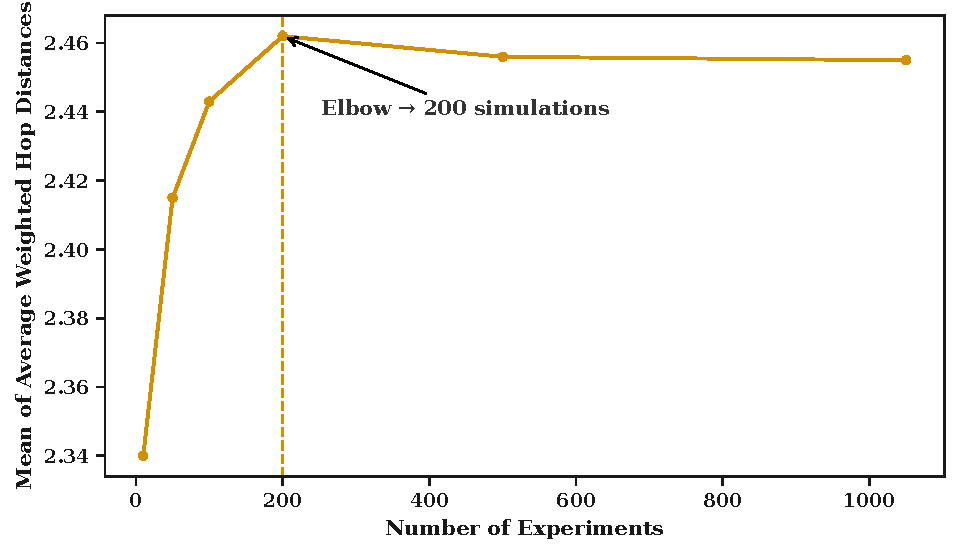
\includegraphics[width=0.85\linewidth]{images/elbow_plot_result.pdf}
% \caption{
% Elbow analysis of the mean weighted proximity distance $\mu_R$ as a function of the number of random simulations $R$. 
% The inflection point around $R = 200$ marks the threshold of convergence, beyond which additional realizations produce negligible improvement in the stability of the null distribution.
% }
% \label{fig:elbow_plot}
% \end{figure}
As summarized in Table~\ref{tab:null_wpd_stats}, the FLO \gls{dcfc} network exhibits a proximity value of 2.8820 hops, compared with a mean of 2.1272 hops across 1,050 randomized placements. Among these trials, 902 configurations (85.7\%) achieved lower \gls{wpd} values, placing the observed network in the lower tail of the null distribution and indicating that its spatial configuration underperforms relative to most random alternatives.
% A broader statistical analysis, based on 1,050 randomized experiments, yields a comparable mean of 2.1261 with a standard deviation of 0.6713. When the FLO DCFC network value is evaluated against this reference random distribution, it corresponds to a z-score of approximately 1.13 and a one-sided p-value of about 0.13, indicating that the observed deviation from random performance is not statistically significant. 
% The Kolmogorov-Smirnov test produces a p-value of 0.0012, revealing that the random metric distribution deviates from normality, and thus non-parametric methods such as permutation or bootstrap analysis provide a more reliable inference framework.
The findings indicate that the spatial arrangement of existing FLO \gls{dcfc} stations does not show strong evidence of systematic optimization when compared to randomly placed scenarios. Instead, the observed pattern seems to stem primarily from infrastructural, regulatory, and planning constraints, rather than from an efficient network-level design. 
Figure~\ref{fig:wpd_min} illustrates random charger configurations that achieve both the lowest and highest proximity metrics. This provides a visual contrast with the FLO \gls{dcfc} network and highlights the range of spatial performance outcomes that can occur under non-optimized siting conditions.
% \begin{figure}[htbp]
%     \centering
%     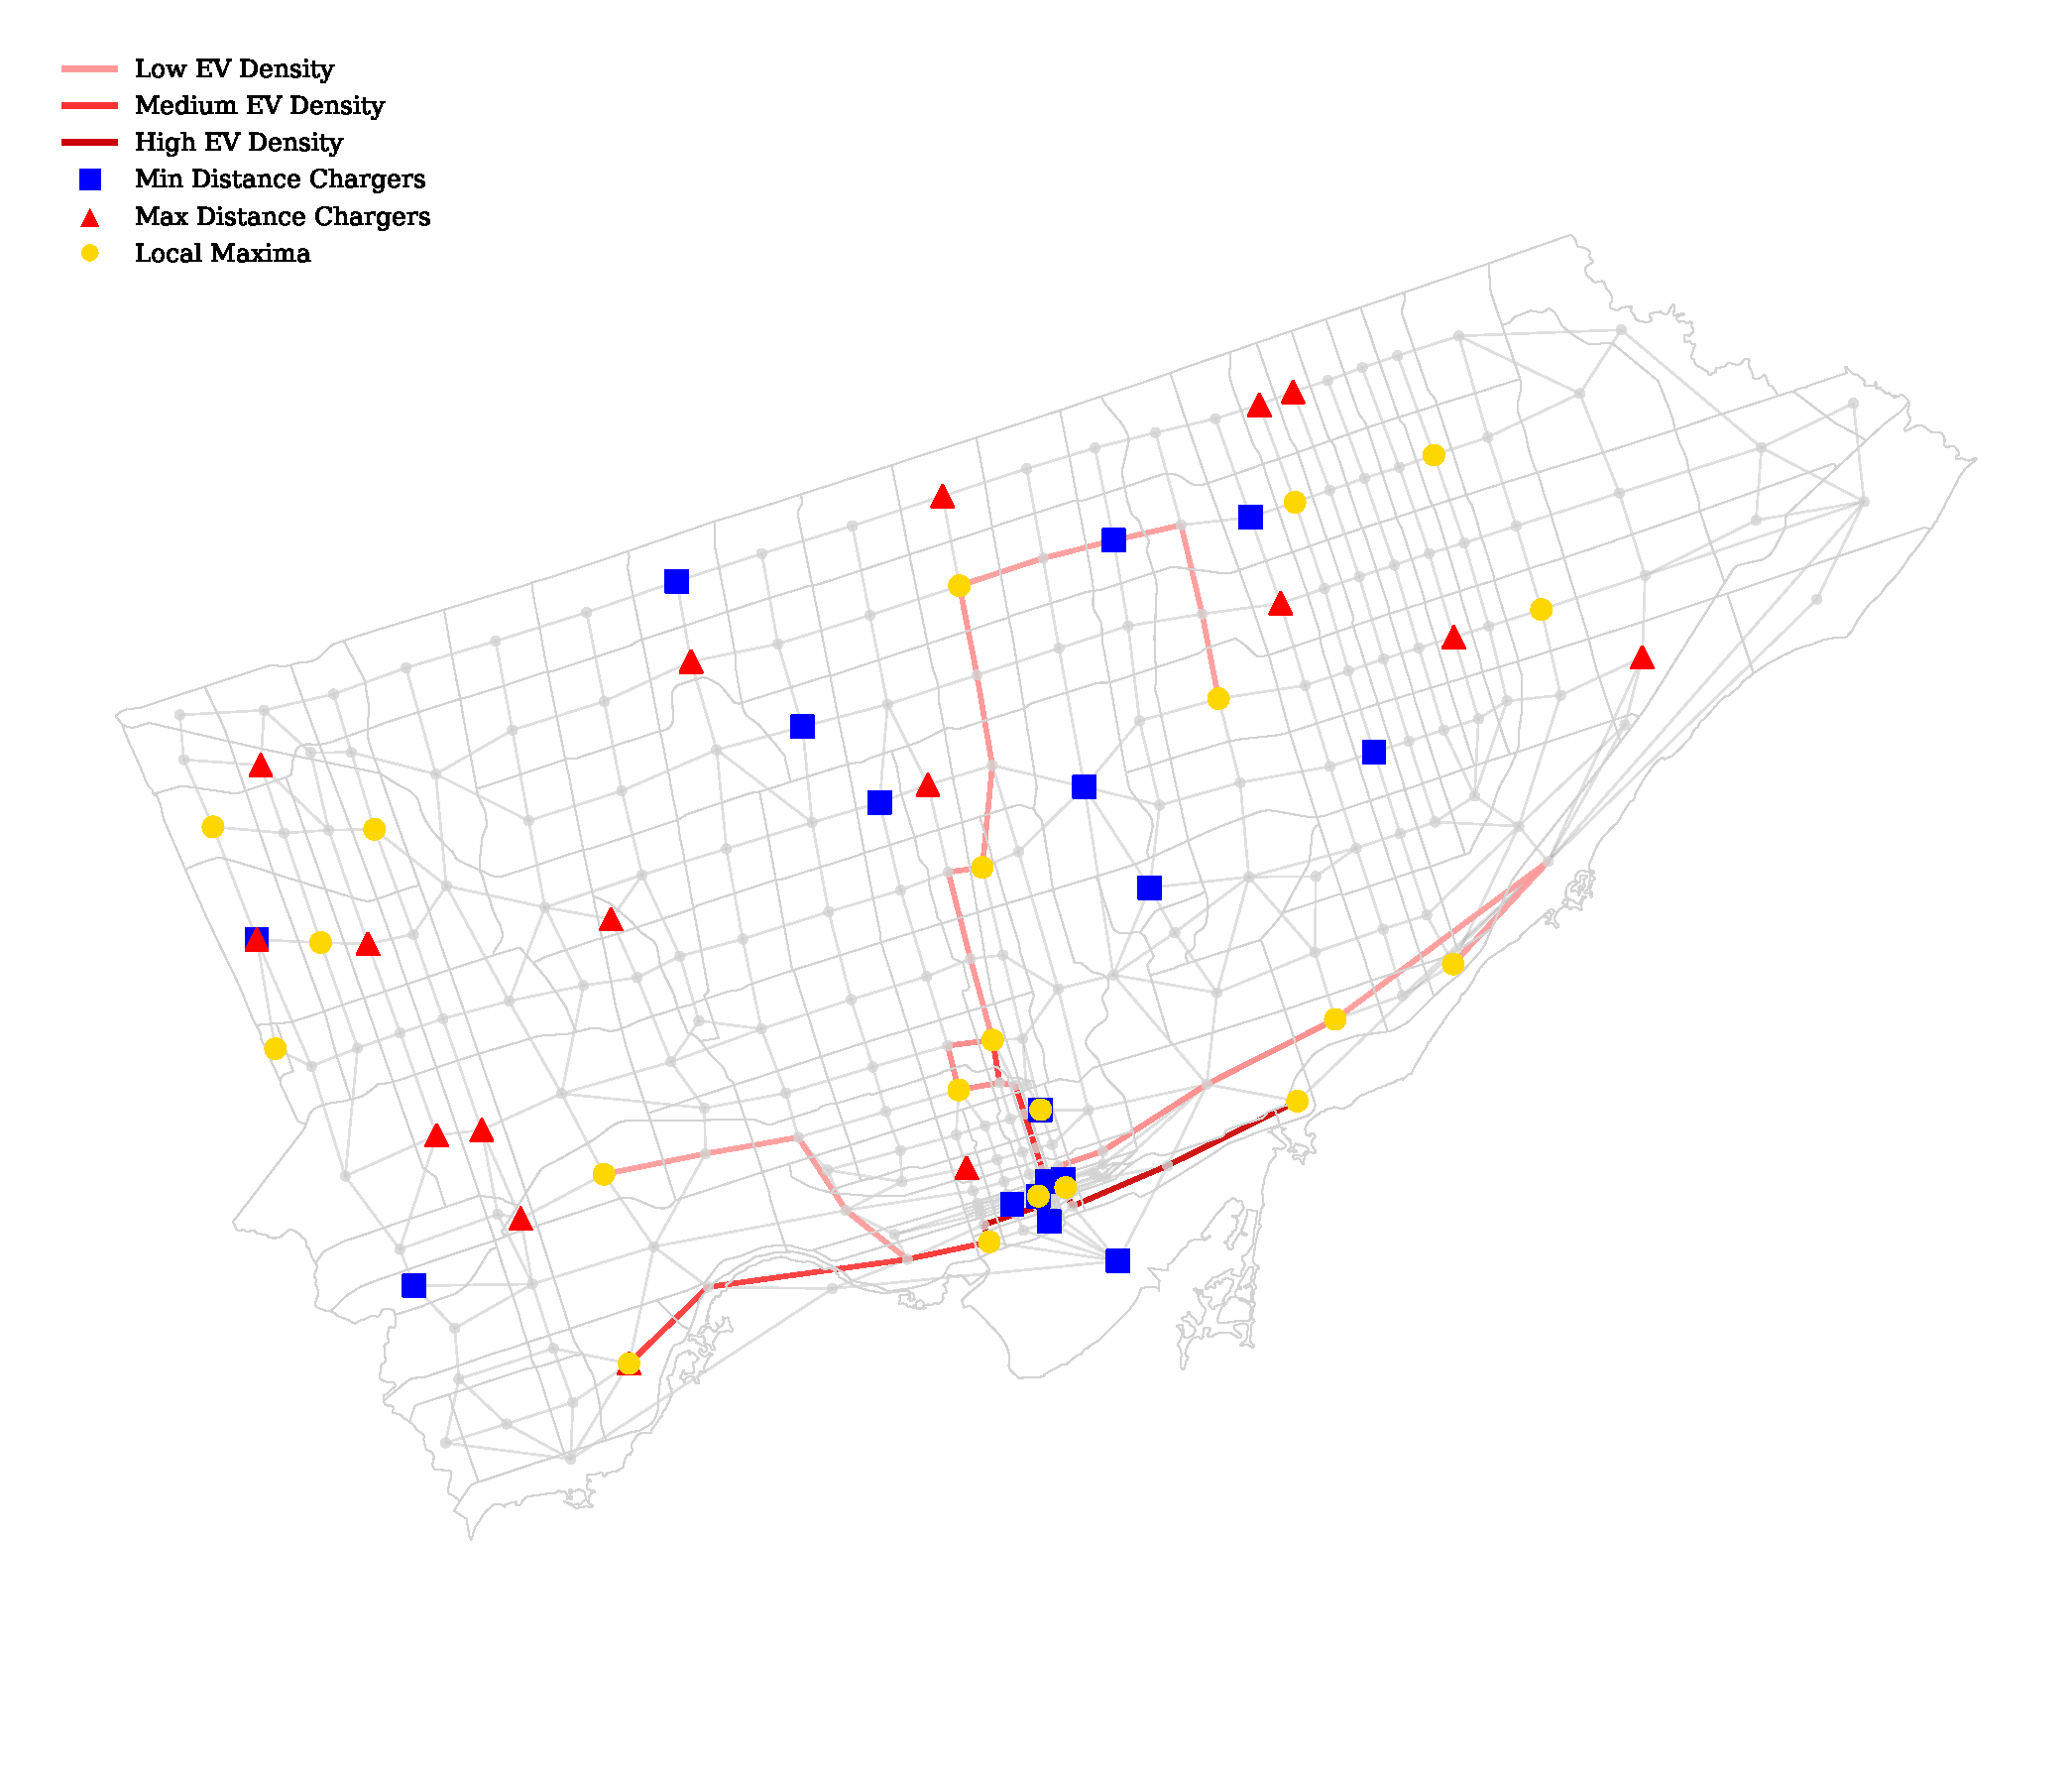
\includegraphics[width=0.85\textwidth]{images/toronto_map_random_chargers.pdf}
%     \caption{Representative random charger layouts corresponding to the lowest and highest computed proximity metrics. 
%     % These configurations provide a visual contrast to the FLO \gls{dcfc} network shown in Figure~\ref{fig:flo_dcfc_map}, 
%     % illustrating how spatial alignment between charger locations and high-activity ridge-path nodes affects the overall proximity efficiency.
%     }
%     \label{fig:wpd_min}
% \end{figure}

\begin{figure}[htbp]
    \centering
    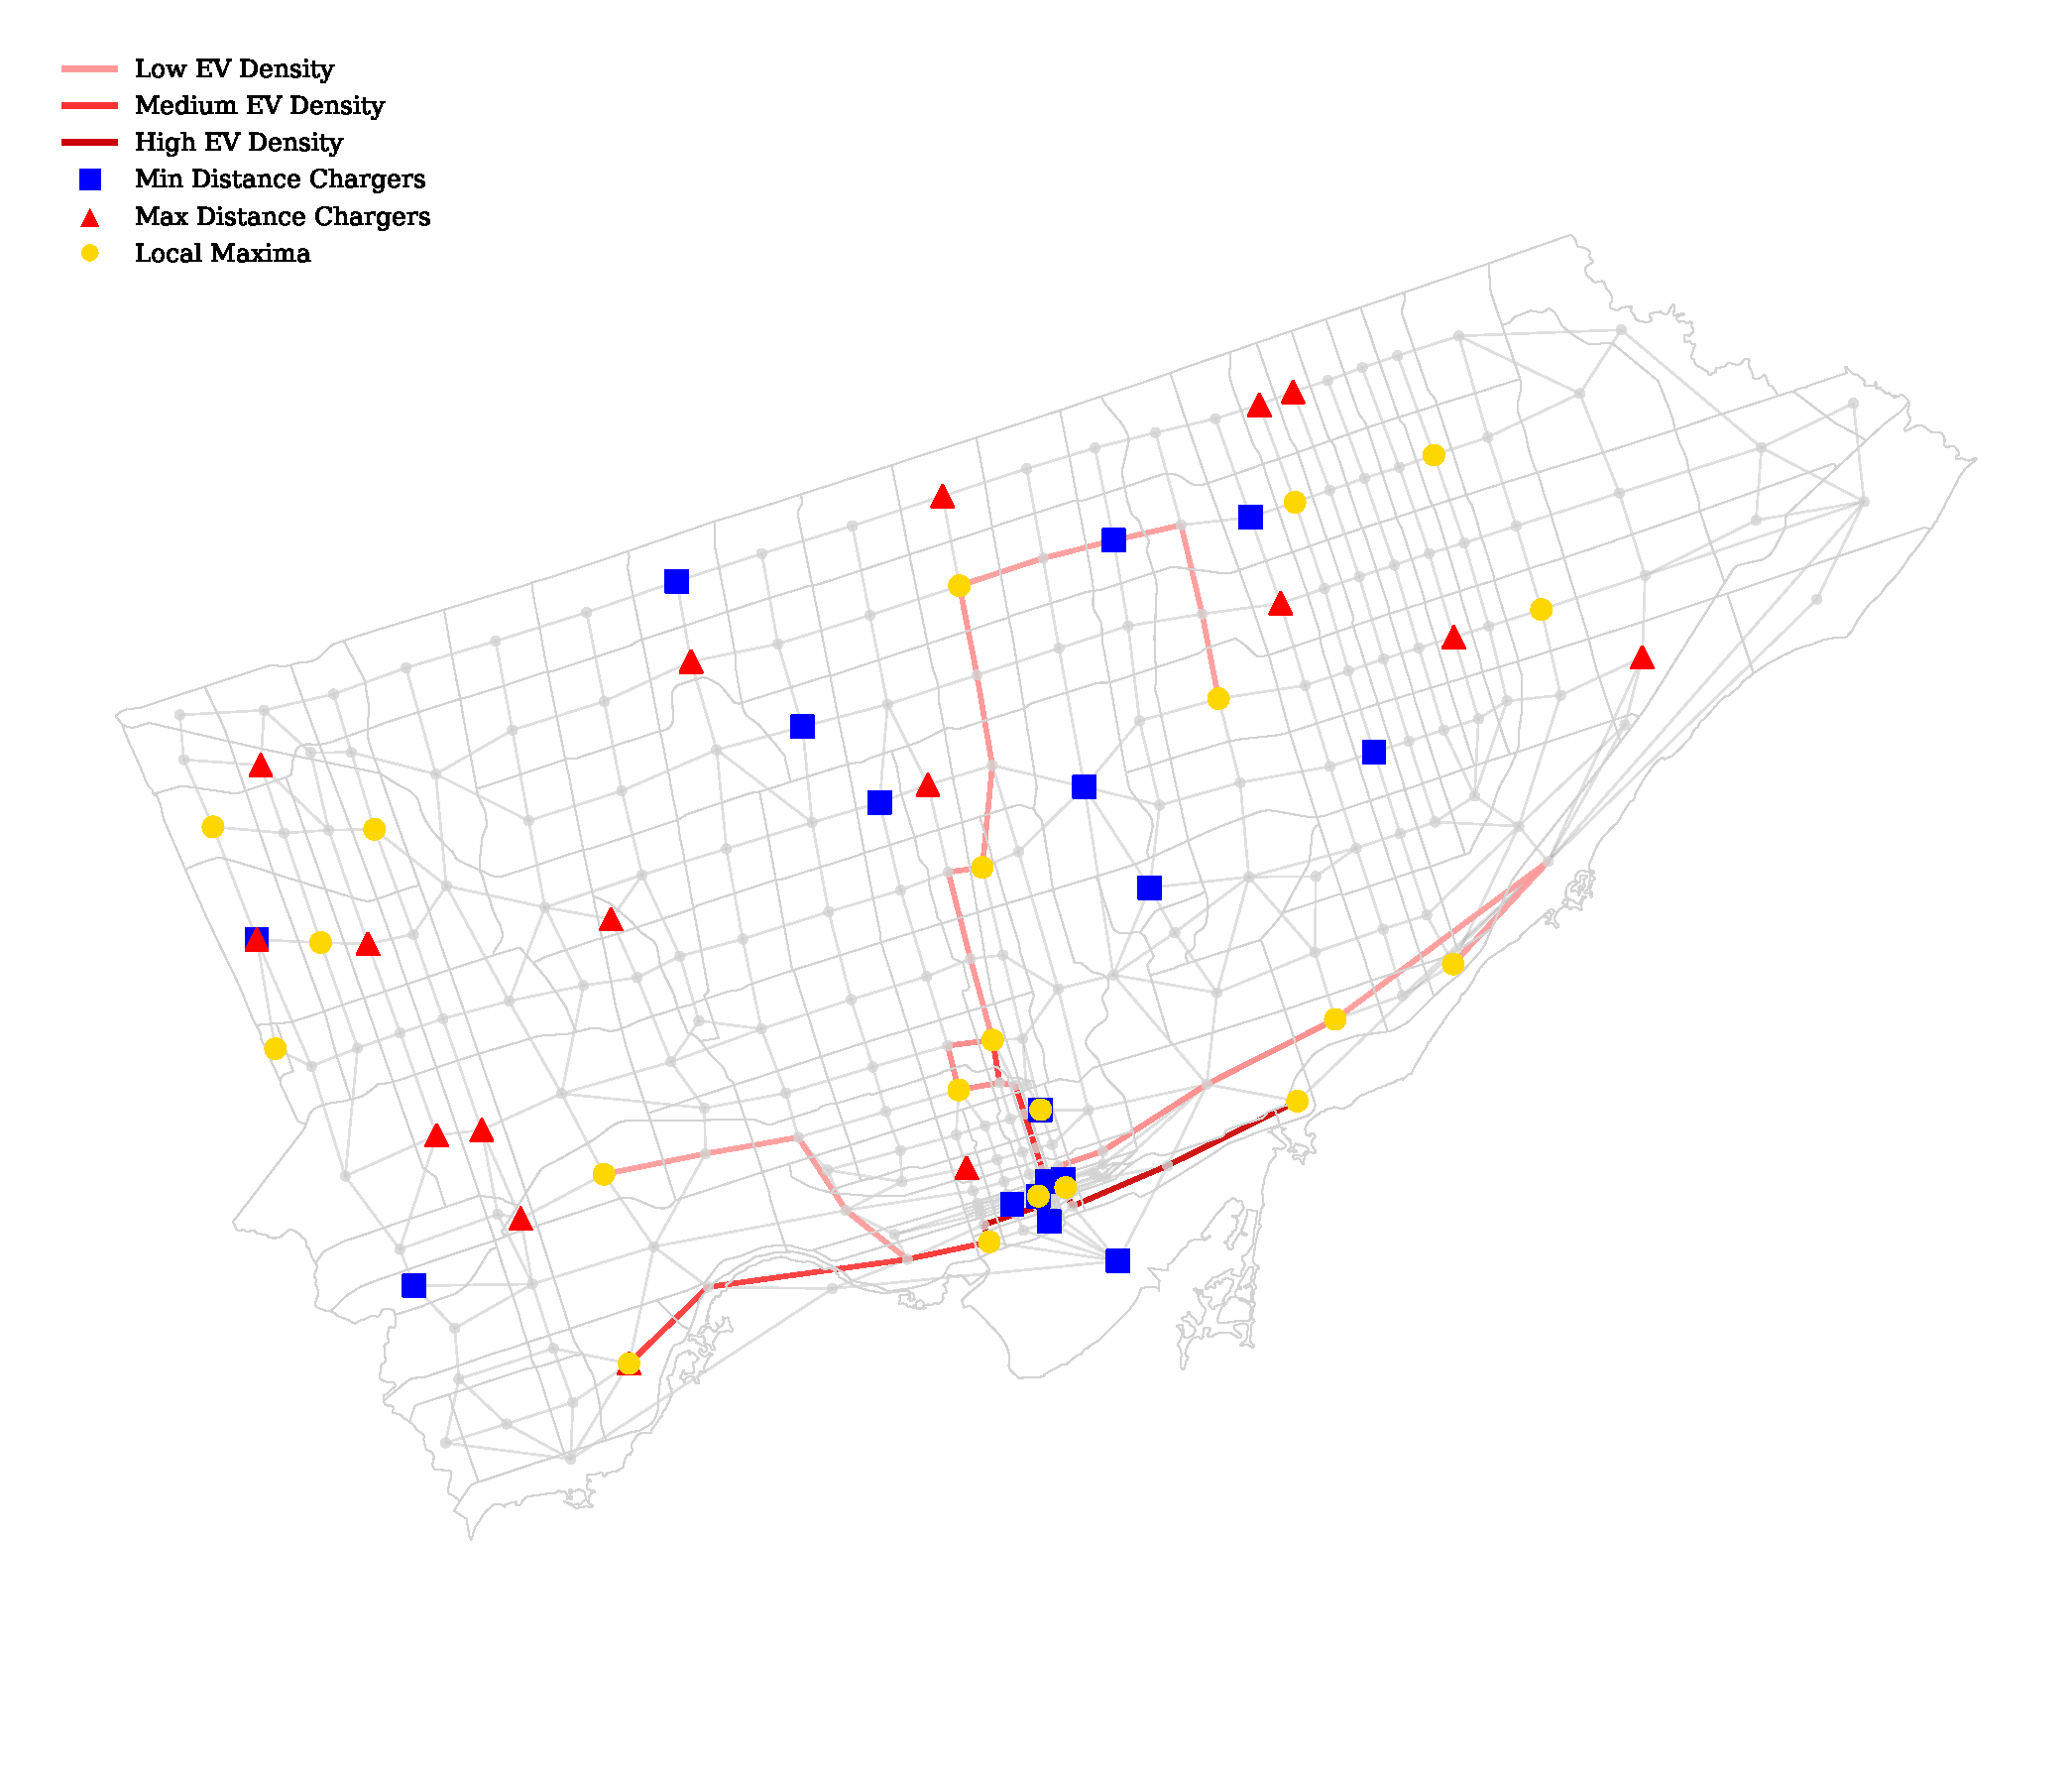
\includegraphics[width=0.7\textwidth, trim={1cm 4cm 1cm 0.8cm}, clip]{images/toronto_map_random_chargers.pdf}
    \caption{Representative random charger layouts corresponding to the lowest and highest computed proximity metrics.}
    \label{fig:wpd_min}
\end{figure}

\begin{table}[htbp]
\centering
\caption{Comprehensive Empirical Evaluation and Statistical Summary of FLO \gls{dcfc} network Proximity Performance}
\label{tab:null_wpd_stats}
\begin{tabularx}{0.9\linewidth}{@{}l>{\centering\arraybackslash}X@{}}
\toprule
\textbf{Metric} & \textbf{Value} \\
\midrule
\multicolumn{2}{@{}l}{\textbf{Empirical Evaluation}} \\[2pt]
FLO \gls{dcfc} network proximity metric (\gls{wpd}$_{\text{FLO}}$) & 2.8820 \\
Total random experiments ($R$) & 1050 \\
Random experiments with lower \gls{wpd} & 902 \\
Empirical percentile rank (\%) & 85.74 \\
Mean of random metrics ($\mathrm{E}[\mathrm{WPD}_{\text{null}}]$) & 2.1272 \\
Standard deviation ($\sigma_{\text{null}}$) & 0.6767 \\
Minimum / Maximum random \gls{wpd}$_{null}$ & 0.7471 / 4.7077 \\[4pt]
% \multicolumn{2}{@{}l}{\textbf{Statistical Inference}} \\[2pt]
% Z-score (normal approximation) & 1.13 \\
% One-sided p-value (Z-test) & 0.1312 \\
% Kolmogorov--Smirnov test p-value & 0.0012 \\
\bottomrule
\end{tabularx}
\end{table}

% -------------------------------------------------
% FIGURE 2: Demand vs. Supply scatter
% -------------------------------------------------
% \begin{figure}[H]
%   \centering
%   \includegraphics[width=0.75\linewidth, keepaspectratio]{figures/demand_supply_scatter.pdf}
%   \caption{Relationship between normalized BEV density ($\widehat{\rho}^{\mathrm{Ar}}_j$) and normalized charger capacity density ($\widehat{\rho}^{\mathrm{Ch}}_j$) across arterial zones. 
%   The dashed line indicates the best-fit regression ($r=0.47$), suggesting moderate spatial alignment between demand intensity and available charging capacity.}
%   \label{fig:demand_supply_scatter}
% \end{figure}

% -------------------------------------------------
% FIGURE 3: Null-model distribution
% -------------------------------------------------
% \begin{figure}[H]
%   \centering
%   \includegraphics[width=0.7\linewidth, keepaspectratio]{figures/null_wpd_distribution.pdf}
%   \caption{Null-model distribution of Weighted Proximity Distance (WPD) generated from 1,000 random charger configurations. 
%   The red vertical line marks the observed $\mathrm{WPD}_{\text{obs}}$, which lies in the lower tail of the null distribution ($p < 0.01$), indicating statistically significant spatial alignment between charger locations and BEV ridge-path demand.}
%   \label{fig:null_wpd}
% \end{figure}

% \subsection{Proximity Performance (Observed)}
% \label{subsec:observed_wpd}
% We compute $\mathrm{WPD}_{\mathrm{real}}$ via Eq.~\eqref{eq:wpd}. The observed value is
% \[
% \mathrm{WPD}_{\mathrm{real}} = \texttt{TODO} \quad \text{(hops)}.
% \]
% Figure~\ref{fig:nearest_assignments} illustrates nearest-charger assignments from ridge nodes.
% \begin{figure}[t]
%   \centering
%   \includegraphics[width=0.92\linewidth]{images/nearest_charger_assignments.pdf}
%   \caption{Nearest-charger assignments from ridge nodes (edges drawn along $G$).}
%   \label{fig:nearest_assignments}
% \end{figure}

% \subsection{Null Distribution and Significance}
% \label{subsec:null_significance}
% We generate $R=\texttt{TODO}$ randomized charger configurations under~\eqref{eq:null_constraints}. 
% The null mean and SD are $\mu_R=\texttt{TODO}$ and $\sigma_R=\texttt{TODO}$ (Eq.~\eqref{eq:null_stats}). 
% The empirical $p$-value (Eq.~\eqref{eq:p_perm}) is
% \[
% p_{\text{perm}} = \texttt{TODO},
% \]
% and the one-sided test~\eqref{eq:hypothesis_test} at $\alpha=0.05$ yields \texttt{Reject/Fail to reject} $H_0$.
% Figure~\ref{fig:null_hist} overlays $\mathrm{WPD}_{\mathrm{real}}$ on the null distribution; Fig.~\ref{fig:elbow_plot} shows elbow convergence of $\mu_R$.

% \begin{figure}[t]
%   \centering
%   \includegraphics[width=0.92\linewidth]{images/null_hist_wpd.pdf}
%   \caption{Null distribution of WPD and observed $\mathrm{WPD}_{\mathrm{real}}$.}
%   \label{fig:null_hist}
% \end{figure}

% \subsection{Sensitivity and Ablation Analyses}
% \label{subsec:sensitivity}
% We probe robustness to modeling choices:
% \begin{enumerate}
%   \item \textbf{$n$-hop smoothing and $\mathbf{w}$:} vary $n\in\{0,1,2,3\}$ and decay patterns; track $\mathrm{WPD}_{\mathrm{real}}$.
%   \item \textbf{Ridge parameters ($\eta,\alpha$):} sweep drop tolerance and max length; report ridge coverage and WPD.
%   \item \textbf{Distance model:} hop vs.\ Euclidean; report $\Delta$WPD.
%   \item \textbf{Supply weighting:} with/without $\widehat{\rho}^{\mathrm{Ch}}$ (capacity-neutral).
%   \item \textbf{Dasymetric refinements:} area vs.\ dwelling/land-use/road-length weights (Appendix sensitivity).
% \end{enumerate}

% \begin{table}[t]
%   \centering
%   \caption{Sensitivity of $\mathrm{WPD}_{\mathrm{real}}$ across modeling choices.}
%   \label{tab:sensitivity}
%   \begin{tabular}{l r r r}
%     \toprule
%     Setting & Param(s) & $\mathrm{WPD}_{\mathrm{real}}$ & $\Delta$ (\%) \\
%     \midrule
%     Baseline & $n=\texttt{TODO}$, $m=\texttt{TODO}$ & \texttt{TODO} & -- \\
%     Hop $\to$ Euclid & -- & \texttt{TODO} & \texttt{TODO} \\
%     No capacity wgt & $w_s\!\to\!1$ & \texttt{TODO} & \texttt{TODO} \\
%     \bottomrule
%   \end{tabular}
% \end{table}

% \subsection{Targeted Corridor Diagnostics (Actionable Gaps)}
% \label{subsec:diagnostics}
% We identify ridge nodes with largest $d_G(v_j,c^*(v_j))$ under high demand $\widehat{\rho}^{\mathrm{Ar}}_j$ and low supply $\widehat{\rho}^{\mathrm{Ch}}$.
% Figure~\ref{fig:gap_map} maps top decile gaps; Table~\ref{tab:corridor_candidates} lists candidate corridors for prioritization.

% \begin{figure}[t]
%   \centering
%   \includegraphics[width=0.92\linewidth]{images/gap_hotspots_map.pdf}
%   \caption{High-demand / low-supply proximity gaps along ridge corridors.}
%   \label{fig:gap_map}
% \end{figure}

% \begin{table}[t]
%   \centering
%   \caption{Candidate corridors for incremental fast-charger deployment.}
%   \label{tab:corridor_candidates}
%   \begin{tabular}{l r r r}
%     \toprule
%     Corridor & Mean demand & Mean supply & Mean distance (hops) \\
%     \midrule
%     \texttt{TODO} & \texttt{TODO} & \texttt{TODO} & \texttt{TODO} \\
%     \bottomrule
%   \end{tabular}
% \end{table}

% \subsection{Computation and Reproducibility}
% \label{subsec:compute_repro}
% Total runtime: \texttt{TODO} (R=\texttt{TODO}); peak memory: \texttt{TODO}.
% Code and parameter files are archived at \texttt{TODO-Repository} with fixed random seeds.
% % TODO: add DOI/Zenodo link if applicable.


\section{Conclusion}
\label{sec:conclusion}
This study has redefined how spatial structure is conceptualized in \gls{bev} \gls{fc} planning by introducing a meso-level, mobility-based framework grounded in arterial mobility network topology. Through the derivation of 234 arterial zones in Toronto, the proposed schema bridges the disconnect between administrative or statical zoning schema and the dynamic nature of \gls{bev} movement. By redistributing ownership data from \glspl{fsa} to these arterial units, the framework constructs a demand field that is directly anchored in urban mobility. Ridge-path extraction then identifies contiguous high-activity corridor zones that represent the structural backbone of BEV activity, while a graph-based proximity analysis quantifies how effectively current infrastructure serves these activity ridges.

Statical benchmarking of Toronto’s existing 17 FLO \gls{dcfc} stations against 1,050 randomized configurations revealed that 85.7\% of random networks achieved shorter weighted proximity distances. This outcome demonstrates that the current network configuration performs no better than random spatial allocation, indicating the absence of systematic spatial optimization in current deployment practices. Despite partial coincidence with major activity zones, the FLO network’s overall alignment with \gls{bev} demand remains weak, highlighting the need for an evidence-based, mobility-aware siting strategy.
Conceptually, the study contributes a scalable, interpretable, and data-efficient foundation for meso-level planning. By coupling arterial-mobility zoning with graph-theoretic analysis, the framework enables multi-criteria evaluation of accessibility, redundancy, and spatial equity without requiring detailed traffic or behavioral datasets. It advances meso-level planning beyond static administrative or grid-based methods, providing a transferable analytical layer that can inform both early-stage infrastructure rollouts and subsequent micro-level optimization models.

Practically, the findings underscore a critical policy implication: current \gls{fc} infrastructure network expansions must evolve from opportunistic placement toward mobility-aligned design. Incorporating arterial road structures into planning can ensure that public and private deployments converge toward regions of highest activity and accessibility. The framework also supports coordination among network operators, enabling municipalities to integrate equity and resilience targets within spatial optimization strategies.
In sum, this research establishes a methodological bridge between macro-level electrification objectives and micro-scale siting models. By anchoring meso-level analysis in the geometry of major urban mobility rather than in administratively or statistically convenient boundaries, it lays a foundation for next-generation planning frameworks that align \gls{bev} charging infrastructure with the actual spatial topology of urban movement.



% This study advances a mobility-based framework for understanding and planning \gls{bev} \gls{fc} infrastructure through the development of a new zoning schema aligned with major arterial roads. The approach maps \gls{bev} ownership counts from administrative units onto these arterial zones, extracts ridge paths from the arterial adjacency graph, and benchmarks network alignment using graph-based proximity metrics. The ridge-extraction pipeline, initiated from local maxima of smoothed \gls{bev} densities , as illustrated in Figure~\ref{fig:local_maxima_map}, reveals distinct, high-activity corridor zones that represent concentrated demand backbones within the urban fabric. The union of ridge-paths' nodes delineates a compact and interpretable backbone of \gls{bev} activity.

% This mobility-based zoning schema complements conventional zoning-based planning by explicitly representing the chain structure of urban \gls{bev} activity and the hop-wise accessibility between activity ridges and charging supply nodes. Results indicate that incremental siting along identified ridge spines can yield pronounced gains in proximity efficiency, particularly where short, high-intensity links integrate into broader corridor networks. Furthermore, this study introduces a new evaluation method based on constructing a null distribution that preserves the fixed number of charger stations and ports, reflecting either existing \gls{dcfc} networks or planned deployments. This enables benchmarking the efficiency of observed or planned networks against randomized charger placements, thereby quantifying how effectively the actual configurations serve \gls{bev} charging demand relative to chance.

% These findings indicate that the existing FLO \gls{dcfc} network does not exhibit spatial optimization relative to potential configurations of comparable scale and capacity. Although charger deployment shows concentration along several \gls{bev}-intensive arterial corridor-zones, the overall placement does not outperform randomized alternatives, revealing a clear gap between the current infrastructure pattern and an optimized spatial configuration. This discrepancy underscores an important research direction-investigating the sources of this gap and the contextual parameters that influence charger siting decisions. Potential contributing factors include business-driven placement priorities, infrastructural and zoning constraints, the coexistence of other \gls{dcfc} networks, and limited coordination among service providers. Understanding these influences is essential for developing data-driven, system-level siting strategies that better align charging supply with \gls{bev} demand along urban arterial corridor-zones.
% Several simplifying assumptions remain. Port power ratings were standardized where station-level specifications were unavailable, potentially understating spatial heterogeneity in delivered capacity. Static BEV density surfaces do not capture temporal fluctuations in activity, and the hop-based metric abstracts away operational constraints such as queuing, power-sharing, and distribution feeder limits. Finally, proximity benchmarking relies on a specific null model and a fixed set of ridge hyperparameters $(L,\eta)$. In sum, the ridge-path lens offers a concise and interpretable backbone of BEV activity that aligns with, but is not yet fully served by, the existing FLO DCFC network. Targeted expansions along undersupplied ridge segments, guided by proximity benchmarks and the future extensions outlined above, present a viable pathway toward higher utilization, equitable access, and grid-aware electrification outcomes.

\section{Future directions}
Future work will extend the proposed meso-level framework along three complementary dimensions: methodological refinement, data integration, and policy application.
From a methodological standpoint, subsequent studies should examine the sensitivity of ridge-path extraction to hyperparameters such as hop distance, drop tolerance, and smoothing weights, as well as explore alternative definitions of adjacency that incorporate traffic flow intensity or functional road hierarchy. The null-distribution benchmarking framework can be expanded to account for spatial clustering, land-use constraints, and power-grid limitations, thereby producing more realistic counterfactual baselines for evaluating charger-activity alignment.

In terms of data integration, future research should incorporate temporal dimensions of \gls{bev} usage, such as diurnal and seasonal charging patterns, by leveraging real charging-session data and mobility traces. Combining these dynamic demand profiles with feeder capacity and transformer headroom models would enable joint optimization of accessibility and grid impact. Emerging graph-learning techniques, including graph neural networks and spatial-temporal embedding models, offer promising avenues for forecasting corridor-level demand and optimizing charger placement under uncertainty.
At the policy level, the framework could support multi-objective planning that simultaneously addresses proximity, equity, resilience, and cost. Comparative case studies across diverse urban forms and governance contexts would help establish typologies of corridor-based \gls{bev} activity and identify transferable siting principles. Ultimately, these extensions aim to transform the proposed framework into a standardized, data-efficient planning tool that informs coordinated, mobility-aligned deployment of \gls{fc} infrastructure in support of large-scale transportation electrification.

% Future research will extend the ridge extraction and proximity analysis framework to incorporate temporal dynamics in \gls{bev} activity. This includes modeling diurnal, weekly, and seasonal variations using charging-session logs and mobility traces to capture time-resolved demand patterns. Nominal port powers will be replaced by site-level ratings with dynamic derating models, while corridor accessibility will be coupled with feeder and transformer headroom to jointly optimize siting and grid impact.

% Further investigations will systematically assess sensitivity to ridge hyperparameters $(L, \eta)$, smoothing choices, and adjacency definitions. Alternative null models that preserve spatial clustering or land-use constraints will be explored to provide more realistic baselines for evaluating spatial performance metrics.
% The WPD metric will be embedded within a broader set of objectives that balance proximity, equity, resiliency, and cost. This multi-objective formulation will enable Pareto analyses for siting strategies that simultaneously serve dense urban cores and underserved peripheral corridors.

% Uncertainty in proximity gains under demand and supply perturbations will be quantified using probabilistic or scenario-based methods. Where feasible, natural experiments or phased deployments will be leveraged to evaluate causal impacts of new charging infrastructure on utilization and accessibility outcomes.
% Validation across diverse urban forms and transportation network topologies will test the transferability of the mobility-based methodology and support the development of typologies that link ridge structures with accessibility and utilization outcomes. Additionally, emerging graph-based learning methods, such as graph neural networks, will be explored to forecast corridor-level demand and recommend capacity expansions under constrained budgets and grid limitations.

% Finally, the research will focus on identifying underlying factors contributing to the observed gap between the existing and optimized fast-charger network configurations. This includes analyzing how business-driven siting priorities, infrastructural and zoning constraints, and the presence of competing \gls{dcfc} networks shape the spatial distribution of chargers. Understanding these parameters will support coordinated, data-driven siting strategies that align charging supply with \gls{bev} activity along urban arterial corridors.


% ----------------------
% References
% ----------------------
% \bibliography{ref}
